\chapter{Badania eksperymentalne}

\section{Zaimplementowane algorytmy}
\subsection{Próbkowanie dwufazowe} \label{section:tp}
Próbkowanie dwufazowe swoją nazwę zawdzięcza procesowi próbkowania składającemu się z dwóch oddzielnych faz
- próbkowania wierzchołków oraz próbkowania krawędzi - wykonywanych jedna po drugiej.
Istotną zaletą tego podejścia jest jego stosunkowo prosta implementacja.

Zaimplementowany algorytm pochodzi z pracy\cite{DBLP:conf/depcos/BozejkoGNAB18}.
Został on przygotowany specjalnie do próbkowania przestrzeni rozwiązań problemu komiwojażera.
Próbkowanie wierzchołków odbywa się poprzez generowanie losowych rozwiązań, a następnie ich optymalizacji algorytmem 2-opt.
Próbkowanie krawędzi polega na wielokrotnym poddaniu każdego ze znalezionych wcześniej lokalnych optimów $n_i$ operacji perturbacji typu 2-exchange,
a następnie poddaniu powstałego rozwiązania optymalizacji algorytmem 2-opt typu \textit{first-improvement} uzyskując w ten sposób lokalne optimum $n_j$.
Następnie dodawana jest krawędź między $n_i$ a $n_j$, lub - jeśli już taka istnieje - jej waga jest zwiększana o 1.

Algorytm przyjmuje trzy parametry: pożądaną liczbę wierzchołków do wygenerowania ($n_{max}$), maksymalną liczbę prób generowania wierzchołka ($n_{att}$)
oraz maksymalną liczbę prób generowania krawędzi($e_{att}$).
Implementacja zastosowana w tej pracy dodatkowo powtarza cały proces kilkukrotnie, za każdym razem zapisując zebrane próbki do pliku.

Algorytm w postaci pseudokodu został przedstawiony na listingu \ref{alg:tp}.

\subsection{Snowball} \label{section:snowball}
Próbkowanie typu Snowball wywodzi się z techniki używanej w badaniach z dziedziny socjologii, w której ludzie należący do próby z populacji
rekrutują kolejnych uczestników badania spośród swoich znajomych.
W kontekście badania przestrzeni rozwiązań technika ta została zaprezentowana w pracy\cite{DBLP:conf/ppsn/VerelDOT18}, gdzie została wykorzystana
do próbkowanie przestrzeni problemu kwadratowego przypisania (QAP).

Próbkowanie składa się z etapów procedury \textit{snowball} próbkującej "wgłąb" i losowego spaceru(ang. \textit{random walk}).
Próbkowanie \textit{snowball} polega na wybraniu rozwiązania startowego i przeszukaniu jego najbliższego sąsiedztwa.
Następnie operacja ta jest powtarzana dla każdego rozwiązania w tym sąsiedztwie. Proces powtarza się aż do osiągnięcia z góry ustalonej głębokości
przeszukiwania. Następnie rozpoczyna się procedura losowego spaceru - wybierane jest kolejne rozwiązanie startowe
ze zbioru sąsiadów poprzedniego rozwiązywania startowego (lub rozwiązanie losowe, jeśli to sąsiedztwo jest puste) i proces \textit{snowball}
rozpoczyna się od nowa. Procedura jest powtarzana aż osiągnięty zostanie z góry ustalony limit długości spaceru.

Zaimplementowany algorytm jest próbą adaptacji tej techniki do zadania przeszukiwania przestrzeni
problemu komiwojażera. Do najważniejszych modyfikacji należy zastąpienie funkcji optymalizacji lokalnej typu \textit{hillclimb}
optymalizacją 2opt, implementacja odpowiedniej funkcji celu oraz operacji mutacji typu 2-exchange.

Algorytm w postaci pseudokodu został przedstawiony na listingu \ref{alg:snowball}.

\vspace{1em}

\begin{algorithm}[H]
    \caption{Próbkowanie dwufazowe - pseudokod}\label{alg:tp}

    \KwData{\\
        \Indp \Indp
        $n_{max}$ - żądana liczba wierzchołków\\
        $n_{att}$ - liczba prób generowania wierzchołków\\
        $e_{att}$ - liczba prób generowania krawędzi\\
        $n_{runs}$ - liczba powtórzeń\\
        $D$ - stała D krawędzi
    }

    \vspace{1em}

    $N \gets \{\}$\;
    $E \gets \{\}$\;
    \For{$i\gets1$ \KwTo $n_{runs}$}{
        $probkujWierzcholki(N, n_{max}, n_{att})$\;
        $probkujKrawedzie(N, E, e_{att})$\;
        $zapiszDoPliku(N, E)$\;
    }
    \vspace{1em}

    \SetKwFunction{FV}{probkujWierzcholki}
    \SetKwProg{Fn}{function}{:}{}

    \Fn{\FV{$N, n_{max}, n_{att}$}}{
        \For{$i\gets1$ \KwTo $n_{max}$}{
            \For{$i\gets1$ \KwTo $n_{att}$}{
                $s \gets losoweRozwiazanie()$\;
                $s \gets 2opt(s)$\;
                $N \gets N \cup \{s\}$\;
            }
        }
    }
    \textbf{end}

    \vspace{1em}

    \SetKwFunction{FE}{probkujKrawedzie}

    \Fn{\FE{$N, E, e_{att}$}}{
        \ForEach{$n \in{N}$}{
            \For{$i\gets1$ \KwTo $e_{att}$}{
                $s \gets 2exchangeMutacja(n, D)$\;
                $s \gets 2optFirstImprovement(s)$\;
                \If{$s \in{N}$}{
                    $E \gets E \cup \{(n, s)\}$\;
                    $w_{ns} \gets w_{ns} + 1$\;
                }
            }
        }
    }
    \textbf{end}

    \vspace{1em}

\end{algorithm}

\begin{algorithm}[p]
    \caption{Próbkowanie snowball - pseudokod}\label{alg:snowball}

    \KwData{\\
        \Indp \Indp
        $w_{len}$ - długość losowego spaceru\\
        $m$ - liczba prób przeszukania sąsiedztwa\\
        $depth$ - głębokość przeszukiwania\\
        $D$ - stała D krawędzi\\
        $s_{tresh}$ - interwał zapisu
    }

    \vspace{1em}
    $s_1 \gets losoweRozwiazanie()$\;
    $n_1 \gets 2opt(s_1)$\;

    $N \gets \{ n_1 \}$\;
    $E \gets \{\}$\;
    \For{$j\gets1$ \KwTo $n_{runs}$}{
        \For{$i\gets1$ \KwTo $w_{len}$}{
            $snowball(n_i, m, depth)$\;
            $n_{i+1} \gets losowySpacer(n_i)$\;
        }
    }
    $zapiszDoPliku(N, E)$\;
    \vspace{1em}

    \SetKwFunction{FS}{snowball}
    \SetKwProg{Fn}{function}{:}{}

    \Fn{\FS{$n, m, depth$}}{
        \If{$d > 0$}{
            \For{$i\gets1$ \KwTo $m$}{
                $s \gets 2opt(2exchangeMutacja(n, D))$\;
                $N \gets N \cup \{ s \}$\;
                \If{$|N| \hspace{0.5em} mod \hspace{0.5em} s_{tresh} = 0$}{
                    $zapiszDoPliku(N, E)$\;
                }
                \uIf{$(n, s) \in{E}$}{
                    $w_{ns} \gets w_{ns} + 1$\;
                }
                \Else{
                    $E \gets E \cup \{ (n, s) \}$\;
                    $w_{ns} \gets 1$\;
                    $snowball(s, m, d-1)$\;
                }
            }
        }
    }
    \textbf{end}

    \vspace{1em}

    \SetKwFunction{FW}{losowySpacer}

    \Fn{\FW{$n_i$}}{
        $neighbours \gets \{ s: (n_i, s) \in E \land s \notin \{ n_0...n_i \} \}$\;
        \uIf{$neighbours \neq \emptyset $}{
            $n_{i+1} \gets losowyElementZeZbioru(neighbours)$\;
        }
        \Else{
            $s \gets losoweRozwiazanie()$\;
            $n_{i+1} \gets 2opt(s)$\;
            $N \gets N \cup \{ n_{i+1} \}$\;
            \If{$|N| \hspace{0.5em} mod \hspace{0.5em} s_{tresh} = 0$}{
                $zapiszDoPliku(N, E)$\;
            }
        }
        \Return $n_{i+1}$
    }
    \textbf{end}

    \vspace{1em}

\end{algorithm}

\newpage

\subsection{Przegląd zupełny}
Ze względu na złożoność problemu komiwojażera przegląd zupełny można zastosować tylko do bardzo małych instancji problemu.
Przegląd polega na wygenerowaniu wszystkich możliwych rozwiązań danej instancji, wykonaniu na nich optymalizacji 2-opt w celu znalezienia
optimów lokalnych a następnie znalezieniu krawędzi oraz obliczeniu ich wag. Dla każdego z rozwiązań generowane są wszystkie
permutacje, które mogą powstać poprzez D-krotne wykonanie na rozwiązaniu operacji 2-exchange. Jeśli wśród tych permutacji znajduje się jedno ze znalezionych wcześniej
lokalnych optimów, oznacza to, że spełniony jest warunek \ref{eq:escape_edge_cond} i dodawana jest nowa krawędź lub zwiększona zostaje waga istniejącej.
Algorytm został przedstawiony na listingu \ref{alg:exhaustive}.

\begin{algorithm}[]
    \caption{Przegląd zupełny}\label{alg:exhaustive}
    $S \gets \{\}$\;
    $P \gets wygenerujWszystkiePermutacje()$\;
    \ForEach{$p \in P$}{
        $lo \gets 2opt(p)$\;
        $S \gets S \cup \{(p, lo)\}$\;
    }

    \SetKwProg{Fn}{function}{:}{}

    \ForEach{$(p, lo) \in S$}{
        \ForEach{$n \in N$}{
            \If{$wZasiegu2Exchange(p, n, D)$}{
                \uIf{$(n, lo) \in E$}{
                    $w_{n, lo} \gets w_{n, lo} + 1$\;
                }\Else{
                    $E \gets E \cup \{(n, lo)\}$\;
                    $w_{n, lo} = 1$\;
                }
            }
        }
    }

    \SetKwFunction{FI}{wZasiegu2Exchange}

    \vspace{1em}

    \Fn{\FI{$p, n, D$}}{
        $permutacje \gets \{p\}$\;
        \For{$i \in 1..D$}{
            $nowe\_perm \gets \{\}$\;
            \ForEach{$perm \in permutacje$}{
                $pochodne\_perm \gets 2exchangeWszystkiePermutacje(permutacje)$\;
                \ForEach{$poch\in pochodne\_perm$}{
                    \If{poch = n}{
                        \Return{true}\;
                    }
                    $nowe\_perm \gets nowe\_perm \cup \{poch\}$\;
                }
            }
            $permutacje \gets nowe\_perm$\;
        }
        \Return{false}\;
    }
    \textbf{end}

\end{algorithm}

\section{Instancje testowe}
Do badań wykorzystano instancje testowe wygenerowane losowo oraz wybrane instancje ze zbioru TSPLIB.
Zaimplementowano trzy generatory tworzące różne typy instancji testowych: z miastami rozłożonymi równomiernie,
z miastami rozłożonymi w klastrach oraz z miastami ułożonymi na siatce.
Wygenerowano instancje testowe każdego z trzech typów instancji losowych o rozmiarach 7, 8, 9, 10, 11 oraz 20, 50, 80 i 100.
Uzyskano w ten sposób 27 instancji problemu.
Ze zbioru TSPLIB wybrano instancje o podobnych rozmiarach: \textbf{burma14}, \textbf{ulysses22}, \textbf{att48}, \textbf{berlin52}, \textbf{pr76}, \textbf{eil76}, \textbf{rat99},
\textbf{bier127}.
W sumie badanie przeprowadzono na 35 instancjach problemu.

\subsection*{Miasta rozmieszczone równomiernie}
Generator losowo rozmieszcza miasta na wirtualnej planszy o ustalonym rozmiarze.\\
Współrzędne miast generowane są losowo z rozkładu równomiernego.
W dalszej części dokumentu instancje wygenerowane tym generatorem będą nazywane \textbf{uniform\_<liczba miast>}.

Przykład wygenerowanej instancji został przedstawiony na rysunku \ref{fig:uniform_example}.

\subsection*{Miasta rozmieszczone w klastrach}
Miasta umieszczane są blisko siebie w kilku grupach oddzielonych większymi odległościami.
W dalszej części dokumentu instancje wygenerowane tym generatorem będą nazywane \textbf{cliques\_<liczba miast>}.
Przykład wygenerowanej instancji został przedstawiony na rysunku \ref{fig:clique_example}.


\subsection*{Miasta rozmieszczone na siatce}
Miasta umieszczane są na siatce, w stałej odległości od swoich sąsiadów.
W dalszej części dokumentu instancje wygenerowane tym generatorem będą nazywane \textbf{grid\_<liczba miast>}.
Przykład wygenerowanej instancji został przedstawiony na rysunku \ref{fig:grid_example}.

\begin{figure}[h!]
    \centering
    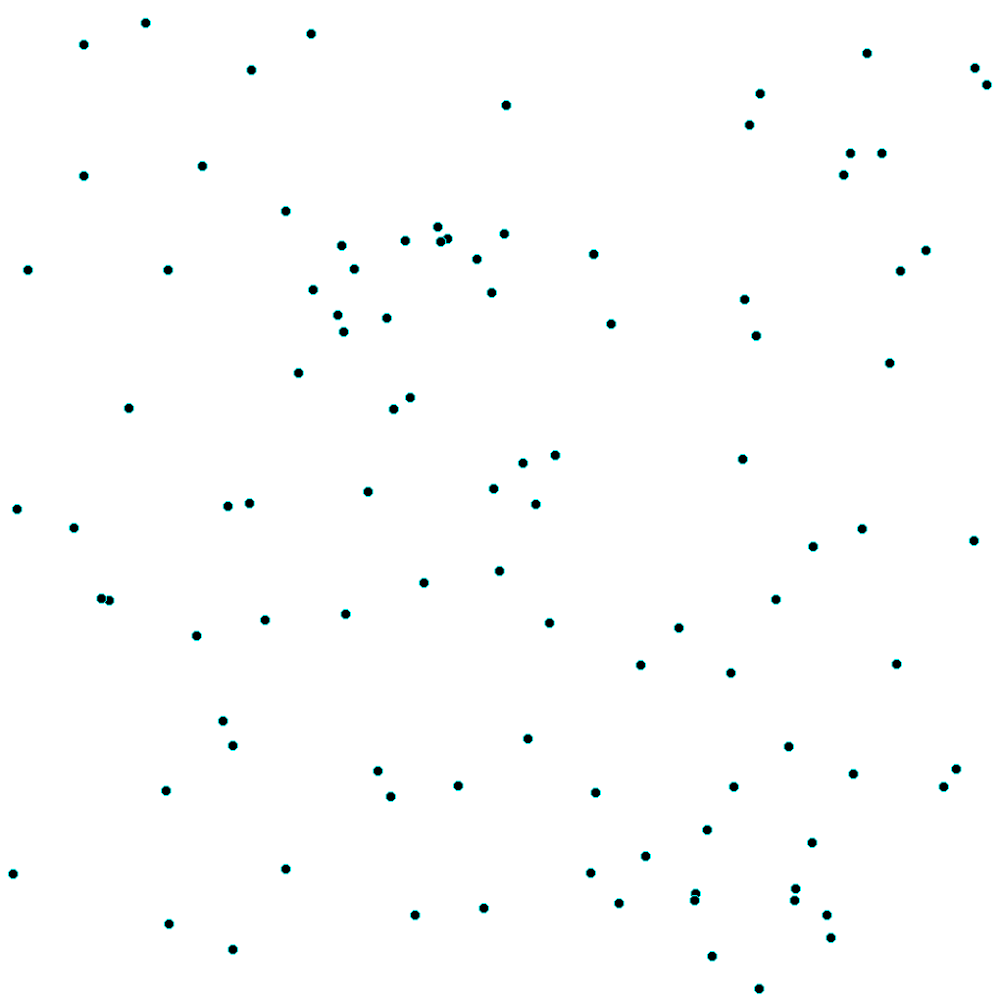
\includegraphics[width=0.46\textwidth]{chapters/experiments/img/uniform_example.png}
    \caption{Wizualizacja przykładowej wygenerowanej instancji z miastami rozmieszczonymi równomiernie dla 100 miast}
    \label{fig:uniform_example}
\end{figure}

\newpage

\begin{figure}[h!]
    \centering
    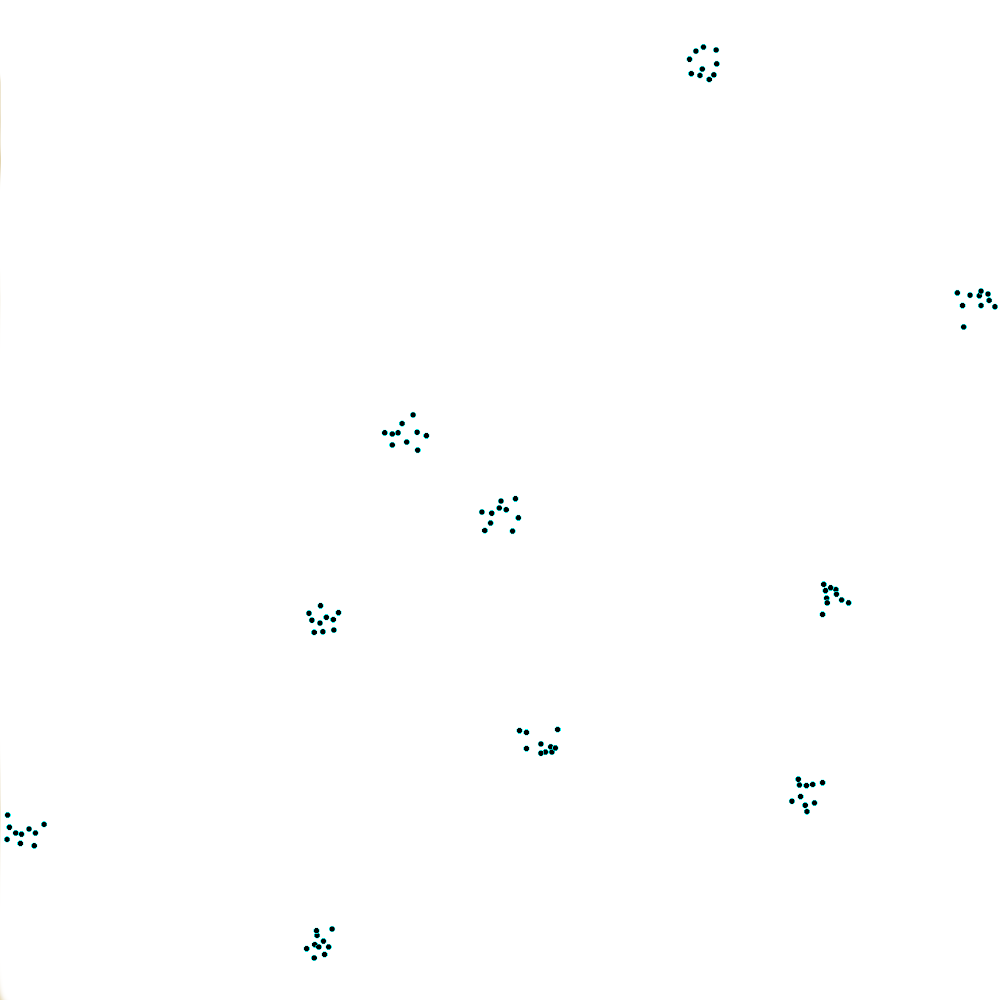
\includegraphics[width=0.60\textwidth]{chapters/experiments/img/clique_example.png}
    \caption{Wizualizacja przykładowej wygenerowanej instancji z miastami rozmieszczonymi w klastrach dla 100 miast}
    \label{fig:clique_example}
\end{figure}

\begin{figure}[h!]
    \centering
    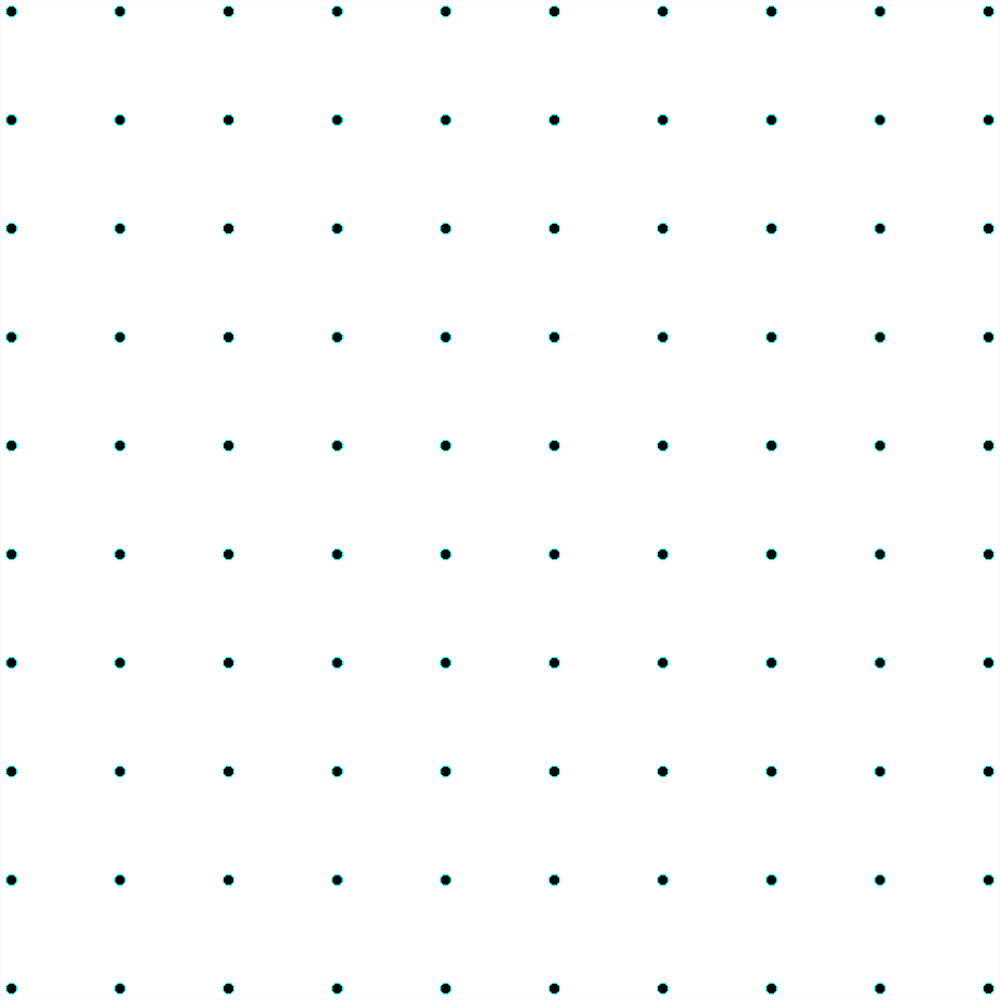
\includegraphics[width=0.60\textwidth]{chapters/experiments/img/grid_example.png}
    \caption{Wizualizacja przykładowej wygenerowanej instancji z miastami rozmieszczonymi na siatce dla 100 miast}
    \label{fig:grid_example}
\end{figure}

\section{Opis badań}

Badania podzielono na trzy etapy: Porównanie wartości metryk z przeglądem zupełnym dla małych instancji,
badanie stabilności średnich instancji, oraz badanie stabilności dużych instancji.

W tym rozdziale przedstawione zostaną tabele i wykresy wygenerowane z wyników próbkowania.
Nazwy metryk są identyczne z nazwami objaśnionymi w rozdziale \ref{sec:metrics}.
Ponadto występują pojęcia:

\begin{itemize}
    \item node\_count - liczba wierzchołków,
    \item edge\_count - liczba krawędzi,
    \item opt\_count - liczba wywołań funkcji 2opt,
    \item oracle\_count - liczba wykonanych obliczeń długości ścieżki (metodą obliczenia przyrostu długości stosowanej w 2opt).
    \item twophase - algorytm dwufazowy
\end{itemize}

Wszystkie badania wykonano wykorzystując model krawędzi typu \textit{Escape Edges} z parametrem $D$ o wartości 2.

\subsection{Porównanie wartości metryk dla małych instancji}
Dla małych instancji wygenerowanych losowo (uniform, grid, cliques) o rozmiarach 7 do 11
możliwe jest wykonanie przeglądu zupełnego.
Na tych instancjach wykonano próbkowanie algorytmami dwufazowym oraz \textit{snowball}, z różnym zestawem parametrów.

Dla algorytmu dwufazowego wykonano próbkowanie dla różnych wartości parametru $n_{max}$ (liczby żądanych wierzchołków): 10, 40, 100 oraz 1000.
Parametry $n_{att}$, $e_{att}$ ustawiono na równe $n_{max}$, a parametr $n_{runs}$ na 1.

Dla algorytmu \textit{snowball} wykonano próbkowanie dla różnych wartości parametru $w_{len}$ (długości losowego spaceru): 1, 10, 100 oraz 1000.
Pozostałe parametry ustawiono następująco: $m$ = 100, $depth$ = 3.

Uzyskane wartości porównano z wartościami uzyskanymi z przeglądu zupełnego.
Wyniki przedstawiono w tabelach od \ref{tab:comp_uniform_7_snowball} do \ref{tab:comp_grid_11_twophase}.
W tabeli przedstawiono wartości metryk uzyskane w przeglądzie zupełnym oraz wartości uzyskane z próbkowania.
Dodatkowo w nawiasie podana została wartość błędu obliczona z wzoru \ref{eq:relError}.
\begin{equation}
    \label{eq:relError}
    E = \frac{|R - S|}{R} \cdot 100\%
\end{equation}
Gdzie:
\begin{itemize}
    \item E - wartość błędu
    \item R - wartość rzeczywista (z przegl. zupełnego)
    \item S - wartość otrzymana z próbkowania.
\end{itemize}

Wartości, dla których błąd nie wyniósł 0 zostały dodatkowo oznaczone w tabeli grubą czcionką.
Przebadano wszystkie miary opisane w sekcji \ref{sec:metrics} za wyjątkiem assortativity\_deg - wartość ta dla małych instancji zwykle przyjmowała
nieprawidłową wartość (NaN), więc zdecydowano o jej wykluczeniu.

\subsubsection{Wyniki}

\begin{table}
\centering
\caption{Instancja uniform\_7 - porównanie wartości miar uzyskanych z próbkowania snowball z wartościami z przeglądu zupełnego.}
\label{tab:comp_uniform_7_snowball}
\footnotesize
\resizebox{\textwidth}{!}{
\begin{tabular}{|l|l|l|l|l|l|}
\hline
\textbf{metryka} & \textbf{p. zupełny} & \textbf{snowball\_1} & \textbf{snowball\_10} & \textbf{snowball\_100} & \textbf{snowball\_1000} \\ \hline
opt\_count & 720.00 & 501.00 & 1608.00 & 10698.00 & 101798.00 \\ \hline
oracle\_count & 42362.00 & 30912.00 & 97125.00 & 650391.00 & 6179229.00 \\ \hline
node\_count & 4.00 & 4.00 (0.00\%) & 4.00 (0.00\%) & 4.00 (0.00\%) & 4.00 (0.00\%) \\ \hline
edge\_count & 16.00 & \textbf{15.00 (6.25\%)} & 16.00 (0.00\%) & 16.00 (0.00\%) & 16.00 (0.00\%) \\ \hline
num\_subsinks & 2.00 & 2.00 (0.00\%) & 2.00 (0.00\%) & 2.00 (0.00\%) & 2.00 (0.00\%) \\ \hline
edge\_to\_node & 4.00 & \textbf{3.75 (6.25\%)} & 4.00 (0.00\%) & 4.00 (0.00\%) & 4.00 (0.00\%) \\ \hline
avg\_fitness & 2720.50 & 2720.50 (0.00\%) & 2720.50 (0.00\%) & 2720.50 (0.00\%) & 2720.50 (0.00\%) \\ \hline
distLO & 0.02 & \textbf{0.05 (203.37\%)} & \textbf{0.02 (2.24\%)} & \textbf{0.00 (79.17\%)} & \textbf{0.00 (97.45\%)} \\ \hline
conrel & 3.00 & 3.00 (0.00\%) & 3.00 (0.00\%) & 3.00 (0.00\%) & 3.00 (0.00\%) \\ \hline
avg\_loop\_weight & 57.00 & \textbf{83.75 (46.93\%)} & \textbf{257.00 (350.88\%)} & \textbf{1863.00 (3168.42\%)} & \textbf{17944.75 (31382.02\%)} \\ \hline
go\_path\_ratio & 0.75 & 0.75 (0.00\%) & 0.75 (0.00\%) & 0.75 (0.00\%) & 0.75 (0.00\%) \\ \hline
avg\_go\_path\_len & 1.00 & 1.00 (0.00\%) & 1.00 (0.00\%) & 1.00 (0.00\%) & 1.00 (0.00\%) \\ \hline
max\_go\_path\_len & 1.00 & 1.00 (0.00\%) & 1.00 (0.00\%) & 1.00 (0.00\%) & 1.00 (0.00\%) \\ \hline
num\_sinks & 2.00 & 2.00 (0.00\%) & 2.00 (0.00\%) & 2.00 (0.00\%) & 2.00 (0.00\%) \\ \hline
num\_sources & 2.00 & 2.00 (0.00\%) & 2.00 (0.00\%) & 2.00 (0.00\%) & 2.00 (0.00\%) \\ \hline
funnel\_num & 2.00 & 2.00 (0.00\%) & 2.00 (0.00\%) & 2.00 (0.00\%) & 2.00 (0.00\%) \\ \hline
mean\_funnel\_size & 3.00 & 3.00 (0.00\%) & 3.00 (0.00\%) & 3.00 (0.00\%) & 3.00 (0.00\%) \\ \hline
max\_funnel\_size & 3.00 & 3.00 (0.00\%) & 3.00 (0.00\%) & 3.00 (0.00\%) & 3.00 (0.00\%) \\ \hline
max\_out\_degree & 3.00 & 3.00 (0.00\%) & 3.00 (0.00\%) & 3.00 (0.00\%) & 3.00 (0.00\%) \\ \hline
avg\_out\_degree & 3.00 & \textbf{2.75 (8.33\%)} & 3.00 (0.00\%) & 3.00 (0.00\%) & 3.00 (0.00\%) \\ \hline
max\_in\_degree & 3.00 & 3.00 (0.00\%) & 3.00 (0.00\%) & 3.00 (0.00\%) & 3.00 (0.00\%) \\ \hline
avg\_in\_degree & 3.00 & \textbf{2.75 (8.33\%)} & 3.00 (0.00\%) & 3.00 (0.00\%) & 3.00 (0.00\%) \\ \hline
density & 1.33 & \textbf{1.25 (6.25\%)} & 1.33 (0.00\%) & 1.33 (0.00\%) & 1.33 (0.00\%) \\ \hline
num\_cc & 1.00 & 1.00 (0.00\%) & 1.00 (0.00\%) & 1.00 (0.00\%) & 1.00 (0.00\%) \\ \hline
largest\_cc & 4.00 & 4.00 (0.00\%) & 4.00 (0.00\%) & 4.00 (0.00\%) & 4.00 (0.00\%) \\ \hline
largest\_cc\_radius & 1.00 & 1.00 (0.00\%) & 1.00 (0.00\%) & 1.00 (0.00\%) & 1.00 (0.00\%) \\ \hline
avg\_path\_len & 1.00 & \textbf{1.08 (8.33\%)} & 1.00 (0.00\%) & 1.00 (0.00\%) & 1.00 (0.00\%) \\ \hline
largest\_clique\_size & 4.00 & 4.00 (0.00\%) & 4.00 (0.00\%) & 4.00 (0.00\%) & 4.00 (0.00\%) \\ \hline
reciprocity & 1.00 & \textbf{0.91 (9.09\%)} & 1.00 (0.00\%) & 1.00 (0.00\%) & 1.00 (0.00\%) \\ \hline
\end{tabular}
}
\end{table}

\begin{table}
\centering
\caption{Instancja uniform\_7 - porównanie wartości miar uzyskanych z próbkowania dwufazowego z wartościami z przeglądu zupełnego.}
\label{tab:comp_uniform_7_twophase}
\footnotesize
\resizebox{\textwidth}{!}{
\begin{tabular}{|l|l|l|l|l|l|}
\hline
\textbf{metryka} & \textbf{p. zupełny} & \textbf{dwufazowy\_10} & \textbf{dwufazowy\_100} & \textbf{dwufazowy\_1000} & \textbf{dwufazowy\_10000} \\ \hline
opt\_count & 720.00 & 107.00 & 10007.00 & 1000014.00 & 100000005.00 \\ \hline
oracle\_count & 42362.00 & 7157.00 & 787632.00 & 79970482.00 & 8007871548.00 \\ \hline
node\_count & 4.00 & 4.00 (0.00\%) & 4.00 (0.00\%) & 4.00 (0.00\%) & 4.00 (0.00\%) \\ \hline
edge\_count & 16.00 & \textbf{10.00 (37.50\%)} & \textbf{15.00 (6.25\%)} & 16.00 (0.00\%) & 16.00 (0.00\%) \\ \hline
num\_subsinks & 2.00 & 2.00 (0.00\%) & 2.00 (0.00\%) & 2.00 (0.00\%) & 2.00 (0.00\%) \\ \hline
edge\_to\_node & 4.00 & \textbf{2.50 (37.50\%)} & \textbf{3.75 (6.25\%)} & 4.00 (0.00\%) & 4.00 (0.00\%) \\ \hline
avg\_fitness & 2720.50 & 2720.50 (0.00\%) & 2720.50 (0.00\%) & 2720.50 (0.00\%) & 2720.50 (0.00\%) \\ \hline
distLO & 0.02 & \textbf{0.42 (2237.80\%)} & \textbf{0.33 (1748.65\%)} & \textbf{0.02 (2.72\%)} & \textbf{0.00 (92.46\%)} \\ \hline
conrel & 3.00 & \textbf{1.00 (66.67\%)} & 3.00 (0.00\%) & 3.00 (0.00\%) & 3.00 (0.00\%) \\ \hline
avg\_loop\_weight & 57.00 & \textbf{4.50 (92.11\%)} & \textbf{44.00 (22.81\%)} & \textbf{387.00 (578.95\%)} & \textbf{3772.00 (6517.54\%)} \\ \hline
go\_path\_ratio & 0.75 & \textbf{0.25 (66.67\%)} & 0.75 (0.00\%) & 0.75 (0.00\%) & 0.75 (0.00\%) \\ \hline
avg\_go\_path\_len & 1.00 & 1.00 (0.00\%) & 1.00 (0.00\%) & 1.00 (0.00\%) & 1.00 (0.00\%) \\ \hline
max\_go\_path\_len & 1.00 & 1.00 (0.00\%) & 1.00 (0.00\%) & 1.00 (0.00\%) & 1.00 (0.00\%) \\ \hline
num\_sinks & 2.00 & 2.00 (0.00\%) & 2.00 (0.00\%) & 2.00 (0.00\%) & 2.00 (0.00\%) \\ \hline
num\_sources & 2.00 & 2.00 (0.00\%) & 2.00 (0.00\%) & 2.00 (0.00\%) & 2.00 (0.00\%) \\ \hline
funnel\_num & 2.00 & 2.00 (0.00\%) & 2.00 (0.00\%) & 2.00 (0.00\%) & 2.00 (0.00\%) \\ \hline
mean\_funnel\_size & 3.00 & \textbf{2.50 (16.67\%)} & 3.00 (0.00\%) & 3.00 (0.00\%) & 3.00 (0.00\%) \\ \hline
max\_funnel\_size & 3.00 & 3.00 (0.00\%) & 3.00 (0.00\%) & 3.00 (0.00\%) & 3.00 (0.00\%) \\ \hline
max\_out\_degree & 3.00 & 3.00 (0.00\%) & 3.00 (0.00\%) & 3.00 (0.00\%) & 3.00 (0.00\%) \\ \hline
avg\_out\_degree & 3.00 & \textbf{1.50 (50.00\%)} & \textbf{2.75 (8.33\%)} & 3.00 (0.00\%) & 3.00 (0.00\%) \\ \hline
max\_in\_degree & 3.00 & 3.00 (0.00\%) & 3.00 (0.00\%) & 3.00 (0.00\%) & 3.00 (0.00\%) \\ \hline
avg\_in\_degree & 3.00 & \textbf{1.50 (50.00\%)} & \textbf{2.75 (8.33\%)} & 3.00 (0.00\%) & 3.00 (0.00\%) \\ \hline
density & 1.33 & \textbf{0.83 (37.50\%)} & \textbf{1.25 (6.25\%)} & 1.33 (0.00\%) & 1.33 (0.00\%) \\ \hline
num\_cc & 1.00 & 1.00 (0.00\%) & 1.00 (0.00\%) & 1.00 (0.00\%) & 1.00 (0.00\%) \\ \hline
largest\_cc & 4.00 & 4.00 (0.00\%) & 4.00 (0.00\%) & 4.00 (0.00\%) & 4.00 (0.00\%) \\ \hline
largest\_cc\_radius & 1.00 & 1.00 (0.00\%) & 1.00 (0.00\%) & 1.00 (0.00\%) & 1.00 (0.00\%) \\ \hline
avg\_path\_len & 1.00 & \textbf{1.14 (14.29\%)} & \textbf{1.08 (8.33\%)} & 1.00 (0.00\%) & 1.00 (0.00\%) \\ \hline
largest\_clique\_size & 4.00 & \textbf{3.00 (25.00\%)} & 4.00 (0.00\%) & 4.00 (0.00\%) & 4.00 (0.00\%) \\ \hline
reciprocity & 1.00 & \textbf{0.33 (66.67\%)} & \textbf{0.91 (9.09\%)} & 1.00 (0.00\%) & 1.00 (0.00\%) \\ \hline
\end{tabular}
}
\end{table}

\begin{table}
\centering
\caption{Instancja uniform\_8 - porównanie wartości miar uzyskanych z próbkowania snowball z wartościami z przeglądu zupełnego.}
\label{tab:comp_uniform_8_snowball}
\footnotesize
\resizebox{\textwidth}{!}{
\begin{tabular}{|l|l|l|l|l|l|}
\hline
\textbf{metryka} & \textbf{p. zupełny} & \textbf{snowball\_1} & \textbf{snowball\_10} & \textbf{snowball\_100} & \textbf{snowball\_1000} \\ \hline
opt\_count & 5040.00 & 401.00 & 1210.00 & 10300.00 & 101200.00 \\ \hline
oracle\_count & 570090.00 & 34384.00 & 106120.00 & 905660.00 & 8916992.00 \\ \hline
node\_count & 2.00 & 2.00 (0.00\%) & 2.00 (0.00\%) & 2.00 (0.00\%) & 2.00 (0.00\%) \\ \hline
edge\_count & 4.00 & 4.00 (0.00\%) & 4.00 (0.00\%) & 4.00 (0.00\%) & 4.00 (0.00\%) \\ \hline
num\_subsinks & 2.00 & 2.00 (0.00\%) & 2.00 (0.00\%) & 2.00 (0.00\%) & 2.00 (0.00\%) \\ \hline
edge\_to\_node & 2.00 & 2.00 (0.00\%) & 2.00 (0.00\%) & 2.00 (0.00\%) & 2.00 (0.00\%) \\ \hline
avg\_fitness & 3224.00 & 3224.00 (0.00\%) & 3224.00 (0.00\%) & 3224.00 (0.00\%) & 3224.00 (0.00\%) \\ \hline
distLO & 0.03 & \textbf{0.02 (15.71\%)} & \textbf{0.01 (65.97\%)} & \textbf{0.00 (96.21\%)} & \textbf{0.00 (99.64\%)} \\ \hline
conrel & 1.00 & 1.00 (0.00\%) & 1.00 (0.00\%) & 1.00 (0.00\%) & 1.00 (0.00\%) \\ \hline
avg\_loop\_weight & 206.00 & \textbf{171.50 (16.75\%)} & \textbf{532.50 (158.50\%)} & \textbf{4520.00 (2094.17\%)} & \textbf{44341.50 (21425.00\%)} \\ \hline
go\_path\_ratio & 0.50 & 0.50 (0.00\%) & 0.50 (0.00\%) & 0.50 (0.00\%) & 0.50 (0.00\%) \\ \hline
avg\_go\_path\_len & 1.00 & 1.00 (0.00\%) & 1.00 (0.00\%) & 1.00 (0.00\%) & 1.00 (0.00\%) \\ \hline
max\_go\_path\_len & 1.00 & 1.00 (0.00\%) & 1.00 (0.00\%) & 1.00 (0.00\%) & 1.00 (0.00\%) \\ \hline
num\_sinks & 2.00 & 2.00 (0.00\%) & 2.00 (0.00\%) & 2.00 (0.00\%) & 2.00 (0.00\%) \\ \hline
num\_sources & 2.00 & 2.00 (0.00\%) & 2.00 (0.00\%) & 2.00 (0.00\%) & 2.00 (0.00\%) \\ \hline
funnel\_num & 2.00 & 2.00 (0.00\%) & 2.00 (0.00\%) & 2.00 (0.00\%) & 2.00 (0.00\%) \\ \hline
mean\_funnel\_size & 1.00 & 1.00 (0.00\%) & 1.00 (0.00\%) & 1.00 (0.00\%) & 1.00 (0.00\%) \\ \hline
max\_funnel\_size & 1.00 & 1.00 (0.00\%) & 1.00 (0.00\%) & 1.00 (0.00\%) & 1.00 (0.00\%) \\ \hline
max\_out\_degree & 1.00 & 1.00 (0.00\%) & 1.00 (0.00\%) & 1.00 (0.00\%) & 1.00 (0.00\%) \\ \hline
avg\_out\_degree & 1.00 & 1.00 (0.00\%) & 1.00 (0.00\%) & 1.00 (0.00\%) & 1.00 (0.00\%) \\ \hline
max\_in\_degree & 1.00 & 1.00 (0.00\%) & 1.00 (0.00\%) & 1.00 (0.00\%) & 1.00 (0.00\%) \\ \hline
avg\_in\_degree & 1.00 & 1.00 (0.00\%) & 1.00 (0.00\%) & 1.00 (0.00\%) & 1.00 (0.00\%) \\ \hline
density & 2.00 & 2.00 (0.00\%) & 2.00 (0.00\%) & 2.00 (0.00\%) & 2.00 (0.00\%) \\ \hline
num\_cc & 1.00 & 1.00 (0.00\%) & 1.00 (0.00\%) & 1.00 (0.00\%) & 1.00 (0.00\%) \\ \hline
largest\_cc & 2.00 & 2.00 (0.00\%) & 2.00 (0.00\%) & 2.00 (0.00\%) & 2.00 (0.00\%) \\ \hline
largest\_cc\_radius & 1.00 & 1.00 (0.00\%) & 1.00 (0.00\%) & 1.00 (0.00\%) & 1.00 (0.00\%) \\ \hline
avg\_path\_len & 1.00 & 1.00 (0.00\%) & 1.00 (0.00\%) & 1.00 (0.00\%) & 1.00 (0.00\%) \\ \hline
largest\_clique\_size & 2.00 & 2.00 (0.00\%) & 2.00 (0.00\%) & 2.00 (0.00\%) & 2.00 (0.00\%) \\ \hline
reciprocity & 1.00 & 1.00 (0.00\%) & 1.00 (0.00\%) & 1.00 (0.00\%) & 1.00 (0.00\%) \\ \hline
\end{tabular}
}
\end{table}

\begin{table}
\centering
\caption{Instancja uniform\_8 - porównanie wartości miar uzyskanych z próbkowania dwufazowego z wartościami z przeglądu zupełnego.}
\label{tab:comp_uniform_8_twophase}
\footnotesize
\resizebox{\textwidth}{!}{
\begin{tabular}{|l|l|l|l|l|l|}
\hline
\textbf{metryka} & \textbf{p. zupełny} & \textbf{dwufazowy\_10} & \textbf{dwufazowy\_100} & \textbf{dwufazowy\_1000} & \textbf{dwufazowy\_10000} \\ \hline
opt\_count & 5040.00 & 102.00 & 10003.00 & 1000002.00 & 100000007.00 \\ \hline
oracle\_count & 570090.00 & 13443.00 & 1461069.00 & 146837491.00 & 14695563426.00 \\ \hline
node\_count & 2.00 & 2.00 (0.00\%) & 2.00 (0.00\%) & 2.00 (0.00\%) & 2.00 (0.00\%) \\ \hline
edge\_count & 4.00 & 4.00 (0.00\%) & 4.00 (0.00\%) & 4.00 (0.00\%) & 4.00 (0.00\%) \\ \hline
num\_subsinks & 2.00 & 2.00 (0.00\%) & 2.00 (0.00\%) & 2.00 (0.00\%) & 2.00 (0.00\%) \\ \hline
edge\_to\_node & 2.00 & 2.00 (0.00\%) & 2.00 (0.00\%) & 2.00 (0.00\%) & 2.00 (0.00\%) \\ \hline
avg\_fitness & 3224.00 & 3224.00 (0.00\%) & 3224.00 (0.00\%) & 3224.00 (0.00\%) & 3224.00 (0.00\%) \\ \hline
distLO & 0.03 & \textbf{0.31 (1020.98\%)} & \textbf{0.10 (256.68\%)} & \textbf{0.01 (48.24\%)} & \textbf{0.00 (99.50\%)} \\ \hline
conrel & 1.00 & 1.00 (0.00\%) & 1.00 (0.00\%) & 1.00 (0.00\%) & 1.00 (0.00\%) \\ \hline
avg\_loop\_weight & 206.00 & \textbf{8.50 (95.87\%)} & \textbf{65.00 (68.45\%)} & \textbf{674.50 (227.43\%)} & \textbf{6772.00 (3187.38\%)} \\ \hline
go\_path\_ratio & 0.50 & 0.50 (0.00\%) & 0.50 (0.00\%) & 0.50 (0.00\%) & 0.50 (0.00\%) \\ \hline
avg\_go\_path\_len & 1.00 & 1.00 (0.00\%) & 1.00 (0.00\%) & 1.00 (0.00\%) & 1.00 (0.00\%) \\ \hline
max\_go\_path\_len & 1.00 & 1.00 (0.00\%) & 1.00 (0.00\%) & 1.00 (0.00\%) & 1.00 (0.00\%) \\ \hline
num\_sinks & 2.00 & 2.00 (0.00\%) & 2.00 (0.00\%) & 2.00 (0.00\%) & 2.00 (0.00\%) \\ \hline
num\_sources & 2.00 & 2.00 (0.00\%) & 2.00 (0.00\%) & 2.00 (0.00\%) & 2.00 (0.00\%) \\ \hline
funnel\_num & 2.00 & 2.00 (0.00\%) & 2.00 (0.00\%) & 2.00 (0.00\%) & 2.00 (0.00\%) \\ \hline
mean\_funnel\_size & 1.00 & 1.00 (0.00\%) & 1.00 (0.00\%) & 1.00 (0.00\%) & 1.00 (0.00\%) \\ \hline
max\_funnel\_size & 1.00 & 1.00 (0.00\%) & 1.00 (0.00\%) & 1.00 (0.00\%) & 1.00 (0.00\%) \\ \hline
max\_out\_degree & 1.00 & 1.00 (0.00\%) & 1.00 (0.00\%) & 1.00 (0.00\%) & 1.00 (0.00\%) \\ \hline
avg\_out\_degree & 1.00 & 1.00 (0.00\%) & 1.00 (0.00\%) & 1.00 (0.00\%) & 1.00 (0.00\%) \\ \hline
max\_in\_degree & 1.00 & 1.00 (0.00\%) & 1.00 (0.00\%) & 1.00 (0.00\%) & 1.00 (0.00\%) \\ \hline
avg\_in\_degree & 1.00 & 1.00 (0.00\%) & 1.00 (0.00\%) & 1.00 (0.00\%) & 1.00 (0.00\%) \\ \hline
density & 2.00 & 2.00 (0.00\%) & 2.00 (0.00\%) & 2.00 (0.00\%) & 2.00 (0.00\%) \\ \hline
num\_cc & 1.00 & 1.00 (0.00\%) & 1.00 (0.00\%) & 1.00 (0.00\%) & 1.00 (0.00\%) \\ \hline
largest\_cc & 2.00 & 2.00 (0.00\%) & 2.00 (0.00\%) & 2.00 (0.00\%) & 2.00 (0.00\%) \\ \hline
largest\_cc\_radius & 1.00 & 1.00 (0.00\%) & 1.00 (0.00\%) & 1.00 (0.00\%) & 1.00 (0.00\%) \\ \hline
avg\_path\_len & 1.00 & 1.00 (0.00\%) & 1.00 (0.00\%) & 1.00 (0.00\%) & 1.00 (0.00\%) \\ \hline
largest\_clique\_size & 2.00 & 2.00 (0.00\%) & 2.00 (0.00\%) & 2.00 (0.00\%) & 2.00 (0.00\%) \\ \hline
reciprocity & 1.00 & 1.00 (0.00\%) & 1.00 (0.00\%) & 1.00 (0.00\%) & 1.00 (0.00\%) \\ \hline
\end{tabular}
}
\end{table}

\begin{table}
\centering
\caption{Instancja uniform\_9 - porównanie wartości miar uzyskanych z próbkowania snowball z wartościami z przeglądu zupełnego.}
\label{tab:comp_uniform_9_snowball}
\footnotesize
\resizebox{\textwidth}{!}{
\begin{tabular}{|l|l|l|l|l|l|}
\hline
\textbf{metryka} & \textbf{p. zupełny} & \textbf{snowball\_1} & \textbf{snowball\_10} & \textbf{snowball\_100} & \textbf{snowball\_1000} \\ \hline
opt\_count & 40320.00 & 401.00 & 1210.00 & 10300.00 & 101200.00 \\ \hline
oracle\_count & 6071702.00 & 44460.00 & 136116.00 & 1165968.00 & 11466720.00 \\ \hline
node\_count & 2.00 & 2.00 (0.00\%) & 2.00 (0.00\%) & 2.00 (0.00\%) & 2.00 (0.00\%) \\ \hline
edge\_count & 4.00 & 4.00 (0.00\%) & 4.00 (0.00\%) & 4.00 (0.00\%) & 4.00 (0.00\%) \\ \hline
num\_subsinks & 2.00 & 2.00 (0.00\%) & 2.00 (0.00\%) & 2.00 (0.00\%) & 2.00 (0.00\%) \\ \hline
edge\_to\_node & 2.00 & 2.00 (0.00\%) & 2.00 (0.00\%) & 2.00 (0.00\%) & 2.00 (0.00\%) \\ \hline
avg\_fitness & 2482.00 & 2482.00 (0.00\%) & 2482.00 (0.00\%) & 2482.00 (0.00\%) & 2482.00 (0.00\%) \\ \hline
distLO & 0.00 & \textbf{0.04 (730.53\%)} & \textbf{0.02 (252.09\%)} & \textbf{0.00 (73.72\%)} & \textbf{0.00 (98.09\%)} \\ \hline
conrel & 1.00 & 1.00 (0.00\%) & 1.00 (0.00\%) & 1.00 (0.00\%) & 1.00 (0.00\%) \\ \hline
avg\_loop\_weight & 390.00 & \textbf{180.50 (53.72\%)} & \textbf{528.00 (35.38\%)} & \textbf{4527.50 (1060.90\%)} & \textbf{44516.00 (11314.36\%)} \\ \hline
go\_path\_ratio & 0.50 & 0.50 (0.00\%) & 0.50 (0.00\%) & 0.50 (0.00\%) & 0.50 (0.00\%) \\ \hline
avg\_go\_path\_len & 1.00 & 1.00 (0.00\%) & 1.00 (0.00\%) & 1.00 (0.00\%) & 1.00 (0.00\%) \\ \hline
max\_go\_path\_len & 1.00 & 1.00 (0.00\%) & 1.00 (0.00\%) & 1.00 (0.00\%) & 1.00 (0.00\%) \\ \hline
num\_sinks & 2.00 & 2.00 (0.00\%) & 2.00 (0.00\%) & 2.00 (0.00\%) & 2.00 (0.00\%) \\ \hline
num\_sources & 2.00 & 2.00 (0.00\%) & 2.00 (0.00\%) & 2.00 (0.00\%) & 2.00 (0.00\%) \\ \hline
funnel\_num & 2.00 & 2.00 (0.00\%) & 2.00 (0.00\%) & 2.00 (0.00\%) & 2.00 (0.00\%) \\ \hline
mean\_funnel\_size & 1.00 & 1.00 (0.00\%) & 1.00 (0.00\%) & 1.00 (0.00\%) & 1.00 (0.00\%) \\ \hline
max\_funnel\_size & 1.00 & 1.00 (0.00\%) & 1.00 (0.00\%) & 1.00 (0.00\%) & 1.00 (0.00\%) \\ \hline
max\_out\_degree & 1.00 & 1.00 (0.00\%) & 1.00 (0.00\%) & 1.00 (0.00\%) & 1.00 (0.00\%) \\ \hline
avg\_out\_degree & 1.00 & 1.00 (0.00\%) & 1.00 (0.00\%) & 1.00 (0.00\%) & 1.00 (0.00\%) \\ \hline
max\_in\_degree & 1.00 & 1.00 (0.00\%) & 1.00 (0.00\%) & 1.00 (0.00\%) & 1.00 (0.00\%) \\ \hline
avg\_in\_degree & 1.00 & 1.00 (0.00\%) & 1.00 (0.00\%) & 1.00 (0.00\%) & 1.00 (0.00\%) \\ \hline
density & 2.00 & 2.00 (0.00\%) & 2.00 (0.00\%) & 2.00 (0.00\%) & 2.00 (0.00\%) \\ \hline
num\_cc & 1.00 & 1.00 (0.00\%) & 1.00 (0.00\%) & 1.00 (0.00\%) & 1.00 (0.00\%) \\ \hline
largest\_cc & 2.00 & 2.00 (0.00\%) & 2.00 (0.00\%) & 2.00 (0.00\%) & 2.00 (0.00\%) \\ \hline
largest\_cc\_radius & 1.00 & 1.00 (0.00\%) & 1.00 (0.00\%) & 1.00 (0.00\%) & 1.00 (0.00\%) \\ \hline
avg\_path\_len & 1.00 & 1.00 (0.00\%) & 1.00 (0.00\%) & 1.00 (0.00\%) & 1.00 (0.00\%) \\ \hline
largest\_clique\_size & 2.00 & 2.00 (0.00\%) & 2.00 (0.00\%) & 2.00 (0.00\%) & 2.00 (0.00\%) \\ \hline
reciprocity & 1.00 & 1.00 (0.00\%) & 1.00 (0.00\%) & 1.00 (0.00\%) & 1.00 (0.00\%) \\ \hline
\end{tabular}
}
\end{table}

\begin{table}
\centering
\caption{Instancja uniform\_9 - porównanie wartości miar uzyskanych z próbkowania dwufazowego z wartościami z przeglądu zupełnego.}
\label{tab:comp_uniform_9_twophase}
\footnotesize
\resizebox{\textwidth}{!}{
\begin{tabular}{|l|l|l|l|l|l|}
\hline
\textbf{metryka} & \textbf{p. zupełny} & \textbf{dwufazowy\_10} & \textbf{dwufazowy\_100} & \textbf{dwufazowy\_1000} & \textbf{dwufazowy\_10000} \\ \hline
opt\_count & 40320.00 & 102.00 & 10002.00 & 1000004.00 & 100000003.00 \\ \hline
oracle\_count & 6071702.00 & 19826.00 & 2100542.00 & 211780859.00 & 21201408685.00 \\ \hline
node\_count & 2.00 & 2.00 (0.00\%) & 2.00 (0.00\%) & 2.00 (0.00\%) & 2.00 (0.00\%) \\ \hline
edge\_count & 4.00 & 4.00 (0.00\%) & 4.00 (0.00\%) & 4.00 (0.00\%) & 4.00 (0.00\%) \\ \hline
num\_subsinks & 2.00 & 2.00 (0.00\%) & 2.00 (0.00\%) & 2.00 (0.00\%) & 2.00 (0.00\%) \\ \hline
edge\_to\_node & 2.00 & 2.00 (0.00\%) & 2.00 (0.00\%) & 2.00 (0.00\%) & 2.00 (0.00\%) \\ \hline
avg\_fitness & 2482.00 & 2482.00 (0.00\%) & 2482.00 (0.00\%) & 2482.00 (0.00\%) & 2482.00 (0.00\%) \\ \hline
distLO & 0.00 & \textbf{0.31 (6479.34\%)} & \textbf{0.03 (542.39\%)} & \textbf{0.00 (40.41\%)} & \textbf{0.00 (93.99\%)} \\ \hline
conrel & 1.00 & 1.00 (0.00\%) & 1.00 (0.00\%) & 1.00 (0.00\%) & 1.00 (0.00\%) \\ \hline
avg\_loop\_weight & 390.00 & \textbf{8.50 (97.82\%)} & \textbf{81.00 (79.23\%)} & \textbf{799.00 (104.87\%)} & \textbf{8078.00 (1971.28\%)} \\ \hline
go\_path\_ratio & 0.50 & 0.50 (0.00\%) & 0.50 (0.00\%) & 0.50 (0.00\%) & 0.50 (0.00\%) \\ \hline
avg\_go\_path\_len & 1.00 & 1.00 (0.00\%) & 1.00 (0.00\%) & 1.00 (0.00\%) & 1.00 (0.00\%) \\ \hline
max\_go\_path\_len & 1.00 & 1.00 (0.00\%) & 1.00 (0.00\%) & 1.00 (0.00\%) & 1.00 (0.00\%) \\ \hline
num\_sinks & 2.00 & 2.00 (0.00\%) & 2.00 (0.00\%) & 2.00 (0.00\%) & 2.00 (0.00\%) \\ \hline
num\_sources & 2.00 & 2.00 (0.00\%) & 2.00 (0.00\%) & 2.00 (0.00\%) & 2.00 (0.00\%) \\ \hline
funnel\_num & 2.00 & 2.00 (0.00\%) & 2.00 (0.00\%) & 2.00 (0.00\%) & 2.00 (0.00\%) \\ \hline
mean\_funnel\_size & 1.00 & 1.00 (0.00\%) & 1.00 (0.00\%) & 1.00 (0.00\%) & 1.00 (0.00\%) \\ \hline
max\_funnel\_size & 1.00 & 1.00 (0.00\%) & 1.00 (0.00\%) & 1.00 (0.00\%) & 1.00 (0.00\%) \\ \hline
max\_out\_degree & 1.00 & 1.00 (0.00\%) & 1.00 (0.00\%) & 1.00 (0.00\%) & 1.00 (0.00\%) \\ \hline
avg\_out\_degree & 1.00 & 1.00 (0.00\%) & 1.00 (0.00\%) & 1.00 (0.00\%) & 1.00 (0.00\%) \\ \hline
max\_in\_degree & 1.00 & 1.00 (0.00\%) & 1.00 (0.00\%) & 1.00 (0.00\%) & 1.00 (0.00\%) \\ \hline
avg\_in\_degree & 1.00 & 1.00 (0.00\%) & 1.00 (0.00\%) & 1.00 (0.00\%) & 1.00 (0.00\%) \\ \hline
density & 2.00 & 2.00 (0.00\%) & 2.00 (0.00\%) & 2.00 (0.00\%) & 2.00 (0.00\%) \\ \hline
num\_cc & 1.00 & 1.00 (0.00\%) & 1.00 (0.00\%) & 1.00 (0.00\%) & 1.00 (0.00\%) \\ \hline
largest\_cc & 2.00 & 2.00 (0.00\%) & 2.00 (0.00\%) & 2.00 (0.00\%) & 2.00 (0.00\%) \\ \hline
largest\_cc\_radius & 1.00 & 1.00 (0.00\%) & 1.00 (0.00\%) & 1.00 (0.00\%) & 1.00 (0.00\%) \\ \hline
avg\_path\_len & 1.00 & 1.00 (0.00\%) & 1.00 (0.00\%) & 1.00 (0.00\%) & 1.00 (0.00\%) \\ \hline
largest\_clique\_size & 2.00 & 2.00 (0.00\%) & 2.00 (0.00\%) & 2.00 (0.00\%) & 2.00 (0.00\%) \\ \hline
reciprocity & 1.00 & 1.00 (0.00\%) & 1.00 (0.00\%) & 1.00 (0.00\%) & 1.00 (0.00\%) \\ \hline
\end{tabular}
}
\end{table}

\begin{table}
\centering
\caption{Instancja uniform\_10 - porównanie wartości miar uzyskanych z próbkowania snowball z wartościami z przeglądu zupełnego.}
\label{tab:comp_uniform_10_snowball}
\footnotesize
\resizebox{\textwidth}{!}{
\begin{tabular}{|l|l|l|l|l|l|}
\hline
\textbf{metryka} & \textbf{p. zupełny} & \textbf{snowball\_1} & \textbf{snowball\_10} & \textbf{snowball\_100} & \textbf{snowball\_1000} \\ \hline
opt\_count & 362880.00 & 601.00 & 2006.00 & 11496.00 & 102496.00 \\ \hline
oracle\_count & 70346836.00 & 86985.00 & 293130.00 & 1674675.00 & 14796000.00 \\ \hline
node\_count & 6.00 & 6.00 (0.00\%) & 6.00 (0.00\%) & 6.00 (0.00\%) & 6.00 (0.00\%) \\ \hline
edge\_count & 35.00 & \textbf{20.00 (42.86\%)} & \textbf{30.00 (14.29\%)} & \textbf{32.00 (8.57\%)} & \textbf{32.00 (8.57\%)} \\ \hline
num\_subsinks & 2.00 & \textbf{3.00 (50.00\%)} & 2.00 (0.00\%) & 2.00 (0.00\%) & 2.00 (0.00\%) \\ \hline
edge\_to\_node & 5.83 & \textbf{3.33 (42.86\%)} & \textbf{5.00 (14.29\%)} & \textbf{5.33 (8.57\%)} & \textbf{5.33 (8.57\%)} \\ \hline
avg\_fitness & 2111.67 & 2111.67 (0.00\%) & 2111.67 (0.00\%) & 2111.67 (0.00\%) & 2111.67 (0.00\%) \\ \hline
distLO & 0.01 & \textbf{0.08 (1073.45\%)} & \textbf{0.13 (1844.98\%)} & \textbf{0.03 (301.38\%)} & \textbf{0.00 (38.98\%)} \\ \hline
conrel & 5.00 & \textbf{1.00 (80.00\%)} & 5.00 (0.00\%) & 5.00 (0.00\%) & 5.00 (0.00\%) \\ \hline
avg\_loop\_weight & 352.50 & \textbf{98.60 (72.03\%)} & \textbf{262.33 (25.58\%)} & \textbf{1550.00 (339.72\%)} & \textbf{14307.83 (3958.96\%)} \\ \hline
go\_path\_ratio & 0.83 & \textbf{0.67 (20.00\%)} & 0.83 (0.00\%) & 0.83 (0.00\%) & 0.83 (0.00\%) \\ \hline
avg\_go\_path\_len & 1.00 & \textbf{1.25 (25.00\%)} & 1.00 (0.00\%) & 1.00 (0.00\%) & 1.00 (0.00\%) \\ \hline
max\_go\_path\_len & 1.00 & \textbf{2.00 (100.00\%)} & 1.00 (0.00\%) & 1.00 (0.00\%) & 1.00 (0.00\%) \\ \hline
num\_sinks & 2.00 & \textbf{3.00 (50.00\%)} & 2.00 (0.00\%) & 2.00 (0.00\%) & 2.00 (0.00\%) \\ \hline
num\_sources & 2.00 & 2.00 (0.00\%) & 2.00 (0.00\%) & 2.00 (0.00\%) & 2.00 (0.00\%) \\ \hline
funnel\_num & 2.00 & \textbf{3.00 (50.00\%)} & 2.00 (0.00\%) & 2.00 (0.00\%) & 2.00 (0.00\%) \\ \hline
mean\_funnel\_size & 5.00 & \textbf{2.67 (46.67\%)} & 5.00 (0.00\%) & 5.00 (0.00\%) & 5.00 (0.00\%) \\ \hline
max\_funnel\_size & 5.00 & \textbf{4.00 (20.00\%)} & 5.00 (0.00\%) & 5.00 (0.00\%) & 5.00 (0.00\%) \\ \hline
max\_out\_degree & 5.00 & 5.00 (0.00\%) & 5.00 (0.00\%) & 5.00 (0.00\%) & 5.00 (0.00\%) \\ \hline
avg\_out\_degree & 4.83 & \textbf{2.50 (48.28\%)} & \textbf{4.00 (17.24\%)} & \textbf{4.33 (10.34\%)} & \textbf{4.33 (10.34\%)} \\ \hline
max\_in\_degree & 5.00 & \textbf{3.00 (40.00\%)} & 5.00 (0.00\%) & 5.00 (0.00\%) & 5.00 (0.00\%) \\ \hline
avg\_in\_degree & 4.83 & \textbf{2.50 (48.28\%)} & \textbf{4.00 (17.24\%)} & \textbf{4.33 (10.34\%)} & \textbf{4.33 (10.34\%)} \\ \hline
density & 1.17 & \textbf{0.67 (42.86\%)} & \textbf{1.00 (14.29\%)} & \textbf{1.07 (8.57\%)} & \textbf{1.07 (8.57\%)} \\ \hline
num\_cc & 1.00 & 1.00 (0.00\%) & 1.00 (0.00\%) & 1.00 (0.00\%) & 1.00 (0.00\%) \\ \hline
largest\_cc & 6.00 & 6.00 (0.00\%) & 6.00 (0.00\%) & 6.00 (0.00\%) & 6.00 (0.00\%) \\ \hline
largest\_cc\_radius & 1.00 & 1.00 (0.00\%) & 1.00 (0.00\%) & 1.00 (0.00\%) & 1.00 (0.00\%) \\ \hline
avg\_path\_len & 1.03 & \textbf{1.48 (43.23\%)} & \textbf{1.20 (16.13\%)} & \textbf{1.13 (9.68\%)} & \textbf{1.13 (9.68\%)} \\ \hline
largest\_clique\_size & 6.00 & \textbf{4.00 (33.33\%)} & 6.00 (0.00\%) & 6.00 (0.00\%) & 6.00 (0.00\%) \\ \hline
reciprocity & 0.97 & \textbf{0.67 (30.95\%)} & \textbf{0.75 (22.32\%)} & \textbf{0.85 (12.36\%)} & \textbf{0.85 (12.36\%)} \\ \hline
\end{tabular}
}
\end{table}

\begin{table}
\centering
\caption{Instancja uniform\_10 - porównanie wartości miar uzyskanych z próbkowania dwufazowego z wartościami z przeglądu zupełnego.}
\label{tab:comp_uniform_10_twophase}
\footnotesize
\resizebox{\textwidth}{!}{
\begin{tabular}{|l|l|l|l|l|l|}
\hline
\textbf{metryka} & \textbf{p. zupełny} & \textbf{dwufazowy\_10} & \textbf{dwufazowy\_100} & \textbf{dwufazowy\_1000} & \textbf{dwufazowy\_10000} \\ \hline
opt\_count & 362880.00 & 122.00 & 10014.00 & 1000027.00 & 100000035.00 \\ \hline
oracle\_count & 70346836.00 & 26110.00 & 2795633.00 & 287853142.00 & 28873812637.00 \\ \hline
node\_count & 6.00 & 6.00 (0.00\%) & 6.00 (0.00\%) & 6.00 (0.00\%) & 6.00 (0.00\%) \\ \hline
edge\_count & 35.00 & \textbf{22.00 (37.14\%)} & \textbf{33.00 (5.71\%)} & \textbf{34.00 (2.86\%)} & 35.00 (0.00\%) \\ \hline
num\_subsinks & 2.00 & 2.00 (0.00\%) & 2.00 (0.00\%) & 2.00 (0.00\%) & 2.00 (0.00\%) \\ \hline
edge\_to\_node & 5.83 & \textbf{3.67 (37.14\%)} & \textbf{5.50 (5.71\%)} & \textbf{5.67 (2.86\%)} & 5.83 (0.00\%) \\ \hline
avg\_fitness & 2111.67 & 2111.67 (0.00\%) & 2111.67 (0.00\%) & 2111.67 (0.00\%) & 2111.67 (0.00\%) \\ \hline
distLO & 0.01 & \textbf{0.50 (7332.43\%)} & \textbf{0.12 (1702.30\%)} & \textbf{0.01 (0.29\%)} & \textbf{0.00 (79.86\%)} \\ \hline
conrel & 5.00 & \textbf{2.00 (60.00\%)} & 5.00 (0.00\%) & 5.00 (0.00\%) & 5.00 (0.00\%) \\ \hline
avg\_loop\_weight & 352.50 & \textbf{4.20 (98.81\%)} & \textbf{36.00 (89.79\%)} & \textbf{404.83 (14.85\%)} & \textbf{4023.33 (1041.37\%)} \\ \hline
go\_path\_ratio & 0.83 & 0.83 (0.00\%) & 0.83 (0.00\%) & 0.83 (0.00\%) & 0.83 (0.00\%) \\ \hline
avg\_go\_path\_len & 1.00 & \textbf{1.40 (40.00\%)} & 1.00 (0.00\%) & 1.00 (0.00\%) & 1.00 (0.00\%) \\ \hline
max\_go\_path\_len & 1.00 & \textbf{2.00 (100.00\%)} & 1.00 (0.00\%) & 1.00 (0.00\%) & 1.00 (0.00\%) \\ \hline
num\_sinks & 2.00 & 2.00 (0.00\%) & 2.00 (0.00\%) & 2.00 (0.00\%) & 2.00 (0.00\%) \\ \hline
num\_sources & 2.00 & 2.00 (0.00\%) & 2.00 (0.00\%) & 2.00 (0.00\%) & 2.00 (0.00\%) \\ \hline
funnel\_num & 2.00 & 2.00 (0.00\%) & 2.00 (0.00\%) & 2.00 (0.00\%) & 2.00 (0.00\%) \\ \hline
mean\_funnel\_size & 5.00 & \textbf{4.50 (10.00\%)} & 5.00 (0.00\%) & 5.00 (0.00\%) & 5.00 (0.00\%) \\ \hline
max\_funnel\_size & 5.00 & 5.00 (0.00\%) & 5.00 (0.00\%) & 5.00 (0.00\%) & 5.00 (0.00\%) \\ \hline
max\_out\_degree & 5.00 & \textbf{4.00 (20.00\%)} & 5.00 (0.00\%) & 5.00 (0.00\%) & 5.00 (0.00\%) \\ \hline
avg\_out\_degree & 4.83 & \textbf{2.83 (41.38\%)} & \textbf{4.50 (6.90\%)} & \textbf{4.67 (3.45\%)} & 4.83 (0.00\%) \\ \hline
max\_in\_degree & 5.00 & 5.00 (0.00\%) & 5.00 (0.00\%) & 5.00 (0.00\%) & 5.00 (0.00\%) \\ \hline
avg\_in\_degree & 4.83 & \textbf{2.83 (41.38\%)} & \textbf{4.50 (6.90\%)} & \textbf{4.67 (3.45\%)} & 4.83 (0.00\%) \\ \hline
density & 1.17 & \textbf{0.73 (37.14\%)} & \textbf{1.10 (5.71\%)} & \textbf{1.13 (2.86\%)} & 1.17 (0.00\%) \\ \hline
num\_cc & 1.00 & 1.00 (0.00\%) & 1.00 (0.00\%) & 1.00 (0.00\%) & 1.00 (0.00\%) \\ \hline
largest\_cc & 6.00 & 6.00 (0.00\%) & 6.00 (0.00\%) & 6.00 (0.00\%) & 6.00 (0.00\%) \\ \hline
largest\_cc\_radius & 1.00 & 1.00 (0.00\%) & 1.00 (0.00\%) & 1.00 (0.00\%) & 1.00 (0.00\%) \\ \hline
avg\_path\_len & 1.03 & \textbf{1.15 (11.29\%)} & \textbf{1.10 (6.45\%)} & \textbf{1.07 (3.23\%)} & 1.03 (0.00\%) \\ \hline
largest\_clique\_size & 6.00 & \textbf{5.00 (16.67\%)} & 6.00 (0.00\%) & 6.00 (0.00\%) & 6.00 (0.00\%) \\ \hline
reciprocity & 0.97 & \textbf{0.47 (51.26\%)} & \textbf{0.89 (7.94\%)} & \textbf{0.93 (3.83\%)} & 0.97 (0.00\%) \\ \hline
\end{tabular}
}
\end{table}

\begin{table}
\centering
\caption{Instancja uniform\_11 - porównanie wartości miar uzyskanych z próbkowania snowball z wartościami z przeglądu zupełnego.}
\label{tab:comp_uniform_11_snowball}
\footnotesize
\resizebox{\textwidth}{!}{
\begin{tabular}{|l|l|l|l|l|l|}
\hline
\textbf{metryka} & \textbf{p. zupełny} & \textbf{snowball\_1} & \textbf{snowball\_10} & \textbf{snowball\_100} & \textbf{snowball\_1000} \\ \hline
opt\_count & 3628800.00 & 401.00 & 1408.00 & 10898.00 & 101698.00 \\ \hline
oracle\_count & 979464676.00 & 72105.00 & 253110.00 & 1986930.00 & 18375555.00 \\ \hline
node\_count & 4.00 & 4.00 (0.00\%) & 4.00 (0.00\%) & 4.00 (0.00\%) & 4.00 (0.00\%) \\ \hline
edge\_count & 16.00 & \textbf{10.00 (37.50\%)} & \textbf{14.00 (12.50\%)} & \textbf{14.00 (12.50\%)} & \textbf{14.00 (12.50\%)} \\ \hline
num\_subsinks & 2.00 & \textbf{3.00 (50.00\%)} & 2.00 (0.00\%) & 2.00 (0.00\%) & 2.00 (0.00\%) \\ \hline
edge\_to\_node & 4.00 & \textbf{2.50 (37.50\%)} & \textbf{3.50 (12.50\%)} & \textbf{3.50 (12.50\%)} & \textbf{3.50 (12.50\%)} \\ \hline
avg\_fitness & 2632.50 & 2632.50 (0.00\%) & 2632.50 (0.00\%) & 2632.50 (0.00\%) & 2632.50 (0.00\%) \\ \hline
distLO & 0.00 & \textbf{0.10 (3840.85\%)} & \textbf{0.10 (3748.92\%)} & \textbf{0.01 (400.38\%)} & \textbf{0.00 (9.32\%)} \\ \hline
conrel & 3.00 & \textbf{1.00 (66.67\%)} & 3.00 (0.00\%) & 3.00 (0.00\%) & 3.00 (0.00\%) \\ \hline
avg\_loop\_weight & 738.25 & \textbf{120.33 (83.70\%)} & \textbf{306.50 (58.48\%)} & \textbf{2400.00 (225.09\%)} & \textbf{23065.00 (3024.28\%)} \\ \hline
go\_path\_ratio & 0.75 & \textbf{0.50 (33.33\%)} & 0.75 (0.00\%) & 0.75 (0.00\%) & 0.75 (0.00\%) \\ \hline
avg\_go\_path\_len & 1.00 & 1.00 (0.00\%) & 1.00 (0.00\%) & 1.00 (0.00\%) & 1.00 (0.00\%) \\ \hline
max\_go\_path\_len & 1.00 & 1.00 (0.00\%) & 1.00 (0.00\%) & 1.00 (0.00\%) & 1.00 (0.00\%) \\ \hline
num\_sinks & 2.00 & \textbf{3.00 (50.00\%)} & 2.00 (0.00\%) & 2.00 (0.00\%) & 2.00 (0.00\%) \\ \hline
num\_sources & 2.00 & 2.00 (0.00\%) & 2.00 (0.00\%) & 2.00 (0.00\%) & 2.00 (0.00\%) \\ \hline
funnel\_num & 2.00 & \textbf{3.00 (50.00\%)} & 2.00 (0.00\%) & 2.00 (0.00\%) & 2.00 (0.00\%) \\ \hline
mean\_funnel\_size & 3.00 & \textbf{1.67 (44.44\%)} & 3.00 (0.00\%) & 3.00 (0.00\%) & 3.00 (0.00\%) \\ \hline
max\_funnel\_size & 3.00 & \textbf{2.00 (33.33\%)} & 3.00 (0.00\%) & 3.00 (0.00\%) & 3.00 (0.00\%) \\ \hline
max\_out\_degree & 3.00 & 3.00 (0.00\%) & 3.00 (0.00\%) & 3.00 (0.00\%) & 3.00 (0.00\%) \\ \hline
avg\_out\_degree & 3.00 & \textbf{1.75 (41.67\%)} & \textbf{2.50 (16.67\%)} & \textbf{2.50 (16.67\%)} & \textbf{2.50 (16.67\%)} \\ \hline
max\_in\_degree & 3.00 & \textbf{2.00 (33.33\%)} & 3.00 (0.00\%) & 3.00 (0.00\%) & 3.00 (0.00\%) \\ \hline
avg\_in\_degree & 3.00 & \textbf{1.75 (41.67\%)} & \textbf{2.50 (16.67\%)} & \textbf{2.50 (16.67\%)} & \textbf{2.50 (16.67\%)} \\ \hline
density & 1.33 & \textbf{0.83 (37.50\%)} & \textbf{1.17 (12.50\%)} & \textbf{1.17 (12.50\%)} & \textbf{1.17 (12.50\%)} \\ \hline
num\_cc & 1.00 & 1.00 (0.00\%) & 1.00 (0.00\%) & 1.00 (0.00\%) & 1.00 (0.00\%) \\ \hline
largest\_cc & 4.00 & 4.00 (0.00\%) & 4.00 (0.00\%) & 4.00 (0.00\%) & 4.00 (0.00\%) \\ \hline
largest\_cc\_radius & 1.00 & 1.00 (0.00\%) & 1.00 (0.00\%) & 1.00 (0.00\%) & 1.00 (0.00\%) \\ \hline
avg\_path\_len & 1.00 & \textbf{1.22 (22.22\%)} & \textbf{1.17 (16.67\%)} & \textbf{1.17 (16.67\%)} & \textbf{1.17 (16.67\%)} \\ \hline
largest\_clique\_size & 4.00 & \textbf{3.00 (25.00\%)} & 4.00 (0.00\%) & 4.00 (0.00\%) & 4.00 (0.00\%) \\ \hline
reciprocity & 1.00 & \textbf{0.57 (42.86\%)} & \textbf{0.80 (20.00\%)} & \textbf{0.80 (20.00\%)} & \textbf{0.80 (20.00\%)} \\ \hline
\end{tabular}
}
\end{table}

\begin{table}
\centering
\caption{Instancja uniform\_11 - porównanie wartości miar uzyskanych z próbkowania dwufazowego z wartościami z przeglądu zupełnego.}
\label{tab:comp_uniform_11_twophase}
\footnotesize
\resizebox{\textwidth}{!}{
\begin{tabular}{|l|l|l|l|l|l|}
\hline
\textbf{metryka} & \textbf{p. zupełny} & \textbf{dwufazowy\_10} & \textbf{dwufazowy\_100} & \textbf{dwufazowy\_1000} & \textbf{dwufazowy\_10000} \\ \hline
opt\_count & 3628800.00 & 116.00 & 10013.00 & 1000010.00 & 100000006.00 \\ \hline
oracle\_count & 979464676.00 & 38001.00 & 4086571.00 & 416049316.00 & 41687797175.00 \\ \hline
node\_count & 4.00 & 4.00 (0.00\%) & 4.00 (0.00\%) & 4.00 (0.00\%) & 4.00 (0.00\%) \\ \hline
edge\_count & 16.00 & \textbf{14.00 (12.50\%)} & \textbf{15.00 (6.25\%)} & 16.00 (0.00\%) & 16.00 (0.00\%) \\ \hline
num\_subsinks & 2.00 & 2.00 (0.00\%) & 2.00 (0.00\%) & 2.00 (0.00\%) & 2.00 (0.00\%) \\ \hline
edge\_to\_node & 4.00 & \textbf{3.50 (12.50\%)} & \textbf{3.75 (6.25\%)} & 4.00 (0.00\%) & 4.00 (0.00\%) \\ \hline
avg\_fitness & 2632.50 & 2632.50 (0.00\%) & 2632.50 (0.00\%) & 2632.50 (0.00\%) & 2632.50 (0.00\%) \\ \hline
distLO & 0.00 & \textbf{0.26 (9820.37\%)} & \textbf{0.03 (1125.95\%)} & \textbf{0.00 (63.37\%)} & \textbf{0.00 (81.38\%)} \\ \hline
conrel & 3.00 & 3.00 (0.00\%) & 3.00 (0.00\%) & 3.00 (0.00\%) & 3.00 (0.00\%) \\ \hline
avg\_loop\_weight & 738.25 & \textbf{4.50 (99.39\%)} & \textbf{48.50 (93.43\%)} & \textbf{451.50 (38.84\%)} & \textbf{4685.00 (534.61\%)} \\ \hline
go\_path\_ratio & 0.75 & 0.75 (0.00\%) & 0.75 (0.00\%) & 0.75 (0.00\%) & 0.75 (0.00\%) \\ \hline
avg\_go\_path\_len & 1.00 & 1.00 (0.00\%) & 1.00 (0.00\%) & 1.00 (0.00\%) & 1.00 (0.00\%) \\ \hline
max\_go\_path\_len & 1.00 & 1.00 (0.00\%) & 1.00 (0.00\%) & 1.00 (0.00\%) & 1.00 (0.00\%) \\ \hline
num\_sinks & 2.00 & 2.00 (0.00\%) & 2.00 (0.00\%) & 2.00 (0.00\%) & 2.00 (0.00\%) \\ \hline
num\_sources & 2.00 & 2.00 (0.00\%) & 2.00 (0.00\%) & 2.00 (0.00\%) & 2.00 (0.00\%) \\ \hline
funnel\_num & 2.00 & 2.00 (0.00\%) & 2.00 (0.00\%) & 2.00 (0.00\%) & 2.00 (0.00\%) \\ \hline
mean\_funnel\_size & 3.00 & 3.00 (0.00\%) & 3.00 (0.00\%) & 3.00 (0.00\%) & 3.00 (0.00\%) \\ \hline
max\_funnel\_size & 3.00 & 3.00 (0.00\%) & 3.00 (0.00\%) & 3.00 (0.00\%) & 3.00 (0.00\%) \\ \hline
max\_out\_degree & 3.00 & 3.00 (0.00\%) & 3.00 (0.00\%) & 3.00 (0.00\%) & 3.00 (0.00\%) \\ \hline
avg\_out\_degree & 3.00 & \textbf{2.50 (16.67\%)} & \textbf{2.75 (8.33\%)} & 3.00 (0.00\%) & 3.00 (0.00\%) \\ \hline
max\_in\_degree & 3.00 & 3.00 (0.00\%) & 3.00 (0.00\%) & 3.00 (0.00\%) & 3.00 (0.00\%) \\ \hline
avg\_in\_degree & 3.00 & \textbf{2.50 (16.67\%)} & \textbf{2.75 (8.33\%)} & 3.00 (0.00\%) & 3.00 (0.00\%) \\ \hline
density & 1.33 & \textbf{1.17 (12.50\%)} & \textbf{1.25 (6.25\%)} & 1.33 (0.00\%) & 1.33 (0.00\%) \\ \hline
num\_cc & 1.00 & 1.00 (0.00\%) & 1.00 (0.00\%) & 1.00 (0.00\%) & 1.00 (0.00\%) \\ \hline
largest\_cc & 4.00 & 4.00 (0.00\%) & 4.00 (0.00\%) & 4.00 (0.00\%) & 4.00 (0.00\%) \\ \hline
largest\_cc\_radius & 1.00 & 1.00 (0.00\%) & 1.00 (0.00\%) & 1.00 (0.00\%) & 1.00 (0.00\%) \\ \hline
avg\_path\_len & 1.00 & \textbf{1.17 (16.67\%)} & \textbf{1.08 (8.33\%)} & 1.00 (0.00\%) & 1.00 (0.00\%) \\ \hline
largest\_clique\_size & 4.00 & 4.00 (0.00\%) & 4.00 (0.00\%) & 4.00 (0.00\%) & 4.00 (0.00\%) \\ \hline
reciprocity & 1.00 & \textbf{0.80 (20.00\%)} & \textbf{0.91 (9.09\%)} & 1.00 (0.00\%) & 1.00 (0.00\%) \\ \hline
\end{tabular}
}
\end{table}

\begin{table}
\centering
\caption{Instancja cliques\_7 - porównanie wartości miar uzyskanych z próbkowania snowball z wartościami z przeglądu zupełnego.}
\label{tab:comp_cliques_7_snowball}
\footnotesize
\resizebox{\textwidth}{!}{
\begin{tabular}{|l|l|l|l|l|l|}
\hline
\textbf{metryka} & \textbf{p. zupełny} & \textbf{snowball\_1} & \textbf{snowball\_10} & \textbf{snowball\_100} & \textbf{snowball\_1000} \\ \hline
opt\_count & 720.00 & 301.00 & 1210.00 & 10300.00 & 101200.00 \\ \hline
oracle\_count & 46570.00 & 19467.00 & 79989.00 & 681198.00 & 6671805.00 \\ \hline
node\_count & 2.00 & 2.00 (0.00\%) & 2.00 (0.00\%) & 2.00 (0.00\%) & 2.00 (0.00\%) \\ \hline
edge\_count & 4.00 & 4.00 (0.00\%) & 4.00 (0.00\%) & 4.00 (0.00\%) & 4.00 (0.00\%) \\ \hline
num\_subsinks & 2.00 & 2.00 (0.00\%) & 2.00 (0.00\%) & 2.00 (0.00\%) & 2.00 (0.00\%) \\ \hline
edge\_to\_node & 2.00 & 2.00 (0.00\%) & 2.00 (0.00\%) & 2.00 (0.00\%) & 2.00 (0.00\%) \\ \hline
avg\_fitness & 2401.00 & 2401.00 (0.00\%) & 2401.00 (0.00\%) & 2401.00 (0.00\%) & 2401.00 (0.00\%) \\ \hline
distLO & 0.02 & \textbf{0.03 (33.15\%)} & \textbf{0.00 (78.81\%)} & \textbf{0.00 (96.68\%)} & \textbf{0.00 (99.70\%)} \\ \hline
conrel & 1.00 & 1.00 (0.00\%) & 1.00 (0.00\%) & 1.00 (0.00\%) & 1.00 (0.00\%) \\ \hline
avg\_loop\_weight & 100.00 & \textbf{121.50 (21.50\%)} & \textbf{489.00 (389.00\%)} & \textbf{4266.00 (4166.00\%)} & \textbf{41638.50 (41538.50\%)} \\ \hline
go\_path\_ratio & 0.50 & 0.50 (0.00\%) & 0.50 (0.00\%) & 0.50 (0.00\%) & 0.50 (0.00\%) \\ \hline
avg\_go\_path\_len & 1.00 & 1.00 (0.00\%) & 1.00 (0.00\%) & 1.00 (0.00\%) & 1.00 (0.00\%) \\ \hline
max\_go\_path\_len & 1.00 & 1.00 (0.00\%) & 1.00 (0.00\%) & 1.00 (0.00\%) & 1.00 (0.00\%) \\ \hline
num\_sinks & 2.00 & 2.00 (0.00\%) & 2.00 (0.00\%) & 2.00 (0.00\%) & 2.00 (0.00\%) \\ \hline
num\_sources & 2.00 & 2.00 (0.00\%) & 2.00 (0.00\%) & 2.00 (0.00\%) & 2.00 (0.00\%) \\ \hline
funnel\_num & 2.00 & 2.00 (0.00\%) & 2.00 (0.00\%) & 2.00 (0.00\%) & 2.00 (0.00\%) \\ \hline
mean\_funnel\_size & 1.00 & 1.00 (0.00\%) & 1.00 (0.00\%) & 1.00 (0.00\%) & 1.00 (0.00\%) \\ \hline
max\_funnel\_size & 1.00 & 1.00 (0.00\%) & 1.00 (0.00\%) & 1.00 (0.00\%) & 1.00 (0.00\%) \\ \hline
max\_out\_degree & 1.00 & 1.00 (0.00\%) & 1.00 (0.00\%) & 1.00 (0.00\%) & 1.00 (0.00\%) \\ \hline
avg\_out\_degree & 1.00 & 1.00 (0.00\%) & 1.00 (0.00\%) & 1.00 (0.00\%) & 1.00 (0.00\%) \\ \hline
max\_in\_degree & 1.00 & 1.00 (0.00\%) & 1.00 (0.00\%) & 1.00 (0.00\%) & 1.00 (0.00\%) \\ \hline
avg\_in\_degree & 1.00 & 1.00 (0.00\%) & 1.00 (0.00\%) & 1.00 (0.00\%) & 1.00 (0.00\%) \\ \hline
density & 2.00 & 2.00 (0.00\%) & 2.00 (0.00\%) & 2.00 (0.00\%) & 2.00 (0.00\%) \\ \hline
num\_cc & 1.00 & 1.00 (0.00\%) & 1.00 (0.00\%) & 1.00 (0.00\%) & 1.00 (0.00\%) \\ \hline
largest\_cc & 2.00 & 2.00 (0.00\%) & 2.00 (0.00\%) & 2.00 (0.00\%) & 2.00 (0.00\%) \\ \hline
largest\_cc\_radius & 1.00 & 1.00 (0.00\%) & 1.00 (0.00\%) & 1.00 (0.00\%) & 1.00 (0.00\%) \\ \hline
avg\_path\_len & 1.00 & 1.00 (0.00\%) & 1.00 (0.00\%) & 1.00 (0.00\%) & 1.00 (0.00\%) \\ \hline
largest\_clique\_size & 2.00 & 2.00 (0.00\%) & 2.00 (0.00\%) & 2.00 (0.00\%) & 2.00 (0.00\%) \\ \hline
reciprocity & 1.00 & 1.00 (0.00\%) & 1.00 (0.00\%) & 1.00 (0.00\%) & 1.00 (0.00\%) \\ \hline
\end{tabular}
}
\end{table}

\begin{table}
\centering
\caption{Instancja cliques\_7 - porównanie wartości miar uzyskanych z próbkowania dwufazowego z wartościami z przeglądu zupełnego.}
\label{tab:comp_cliques_7_twophase}
\footnotesize
\resizebox{\textwidth}{!}{
\begin{tabular}{|l|l|l|l|l|l|}
\hline
\textbf{metryka} & \textbf{p. zupełny} & \textbf{dwufazowy\_10} & \textbf{dwufazowy\_100} & \textbf{dwufazowy\_1000} & \textbf{dwufazowy\_10000} \\ \hline
opt\_count & 720.00 & 102.00 & 10004.00 & 1000003.00 & 100000002.00 \\ \hline
oracle\_count & 46570.00 & 8360.00 & 891012.00 & 89532059.00 & 8961919004.00 \\ \hline
node\_count & 2.00 & 2.00 (0.00\%) & 2.00 (0.00\%) & 2.00 (0.00\%) & 2.00 (0.00\%) \\ \hline
edge\_count & 4.00 & 4.00 (0.00\%) & 4.00 (0.00\%) & 4.00 (0.00\%) & 4.00 (0.00\%) \\ \hline
num\_subsinks & 2.00 & 2.00 (0.00\%) & 2.00 (0.00\%) & 2.00 (0.00\%) & 2.00 (0.00\%) \\ \hline
edge\_to\_node & 2.00 & 2.00 (0.00\%) & 2.00 (0.00\%) & 2.00 (0.00\%) & 2.00 (0.00\%) \\ \hline
avg\_fitness & 2401.00 & 2401.00 (0.00\%) & 2401.00 (0.00\%) & 2401.00 (0.00\%) & 2401.00 (0.00\%) \\ \hline
distLO & 0.02 & \textbf{0.60 (2486.90\%)} & \textbf{0.07 (187.43\%)} & \textbf{0.00 (82.76\%)} & \textbf{0.00 (99.21\%)} \\ \hline
conrel & 1.00 & 1.00 (0.00\%) & 1.00 (0.00\%) & 1.00 (0.00\%) & 1.00 (0.00\%) \\ \hline
avg\_loop\_weight & 100.00 & \textbf{7.00 (93.00\%)} & \textbf{68.00 (32.00\%)} & \textbf{713.50 (613.50\%)} & \textbf{7138.00 (7038.00\%)} \\ \hline
go\_path\_ratio & 0.50 & 0.50 (0.00\%) & 0.50 (0.00\%) & 0.50 (0.00\%) & 0.50 (0.00\%) \\ \hline
avg\_go\_path\_len & 1.00 & 1.00 (0.00\%) & 1.00 (0.00\%) & 1.00 (0.00\%) & 1.00 (0.00\%) \\ \hline
max\_go\_path\_len & 1.00 & 1.00 (0.00\%) & 1.00 (0.00\%) & 1.00 (0.00\%) & 1.00 (0.00\%) \\ \hline
num\_sinks & 2.00 & 2.00 (0.00\%) & 2.00 (0.00\%) & 2.00 (0.00\%) & 2.00 (0.00\%) \\ \hline
num\_sources & 2.00 & 2.00 (0.00\%) & 2.00 (0.00\%) & 2.00 (0.00\%) & 2.00 (0.00\%) \\ \hline
funnel\_num & 2.00 & 2.00 (0.00\%) & 2.00 (0.00\%) & 2.00 (0.00\%) & 2.00 (0.00\%) \\ \hline
mean\_funnel\_size & 1.00 & 1.00 (0.00\%) & 1.00 (0.00\%) & 1.00 (0.00\%) & 1.00 (0.00\%) \\ \hline
max\_funnel\_size & 1.00 & 1.00 (0.00\%) & 1.00 (0.00\%) & 1.00 (0.00\%) & 1.00 (0.00\%) \\ \hline
max\_out\_degree & 1.00 & 1.00 (0.00\%) & 1.00 (0.00\%) & 1.00 (0.00\%) & 1.00 (0.00\%) \\ \hline
avg\_out\_degree & 1.00 & 1.00 (0.00\%) & 1.00 (0.00\%) & 1.00 (0.00\%) & 1.00 (0.00\%) \\ \hline
max\_in\_degree & 1.00 & 1.00 (0.00\%) & 1.00 (0.00\%) & 1.00 (0.00\%) & 1.00 (0.00\%) \\ \hline
avg\_in\_degree & 1.00 & 1.00 (0.00\%) & 1.00 (0.00\%) & 1.00 (0.00\%) & 1.00 (0.00\%) \\ \hline
density & 2.00 & 2.00 (0.00\%) & 2.00 (0.00\%) & 2.00 (0.00\%) & 2.00 (0.00\%) \\ \hline
num\_cc & 1.00 & 1.00 (0.00\%) & 1.00 (0.00\%) & 1.00 (0.00\%) & 1.00 (0.00\%) \\ \hline
largest\_cc & 2.00 & 2.00 (0.00\%) & 2.00 (0.00\%) & 2.00 (0.00\%) & 2.00 (0.00\%) \\ \hline
largest\_cc\_radius & 1.00 & 1.00 (0.00\%) & 1.00 (0.00\%) & 1.00 (0.00\%) & 1.00 (0.00\%) \\ \hline
avg\_path\_len & 1.00 & 1.00 (0.00\%) & 1.00 (0.00\%) & 1.00 (0.00\%) & 1.00 (0.00\%) \\ \hline
largest\_clique\_size & 2.00 & 2.00 (0.00\%) & 2.00 (0.00\%) & 2.00 (0.00\%) & 2.00 (0.00\%) \\ \hline
reciprocity & 1.00 & 1.00 (0.00\%) & 1.00 (0.00\%) & 1.00 (0.00\%) & 1.00 (0.00\%) \\ \hline
\end{tabular}
}
\end{table}

\begin{table}
\centering
\caption{Instancja cliques\_8 - porównanie wartości miar uzyskanych z próbkowania snowball z wartościami z przeglądu zupełnego.}
\label{tab:comp_cliques_8_snowball}
\footnotesize
\resizebox{\textwidth}{!}{
\begin{tabular}{|l|l|l|l|l|l|}
\hline
\textbf{metryka} & \textbf{p. zupełny} & \textbf{snowball\_1} & \textbf{snowball\_10} & \textbf{snowball\_100} & \textbf{snowball\_1000} \\ \hline
opt\_count & 5040.00 & 501.00 & 1508.00 & 10598.00 & 101498.00 \\ \hline
oracle\_count & 419679.00 & 42252.00 & 127932.00 & 895076.00 & 8632344.00 \\ \hline
node\_count & 4.00 & 4.00 (0.00\%) & 4.00 (0.00\%) & 4.00 (0.00\%) & 4.00 (0.00\%) \\ \hline
edge\_count & 16.00 & \textbf{15.00 (6.25\%)} & 16.00 (0.00\%) & 16.00 (0.00\%) & 16.00 (0.00\%) \\ \hline
num\_subsinks & 2.00 & 2.00 (0.00\%) & 2.00 (0.00\%) & 2.00 (0.00\%) & 2.00 (0.00\%) \\ \hline
edge\_to\_node & 4.00 & \textbf{3.75 (6.25\%)} & 4.00 (0.00\%) & 4.00 (0.00\%) & 4.00 (0.00\%) \\ \hline
avg\_fitness & 1718.00 & 1718.00 (0.00\%) & 1718.00 (0.00\%) & 1718.00 (0.00\%) & 1718.00 (0.00\%) \\ \hline
distLO & 0.01 & \textbf{0.06 (388.30\%)} & \textbf{0.01 (14.48\%)} & \textbf{0.01 (56.23\%)} & \textbf{0.00 (97.32\%)} \\ \hline
conrel & 3.00 & 3.00 (0.00\%) & 3.00 (0.00\%) & 3.00 (0.00\%) & 3.00 (0.00\%) \\ \hline
avg\_loop\_weight & 141.75 & \textbf{82.25 (41.98\%)} & \textbf{247.00 (74.25\%)} & \textbf{1991.75 (1305.11\%)} & \textbf{19076.00 (13357.50\%)} \\ \hline
go\_path\_ratio & 0.75 & 0.75 (0.00\%) & 0.75 (0.00\%) & 0.75 (0.00\%) & 0.75 (0.00\%) \\ \hline
avg\_go\_path\_len & 1.00 & 1.00 (0.00\%) & 1.00 (0.00\%) & 1.00 (0.00\%) & 1.00 (0.00\%) \\ \hline
max\_go\_path\_len & 1.00 & 1.00 (0.00\%) & 1.00 (0.00\%) & 1.00 (0.00\%) & 1.00 (0.00\%) \\ \hline
num\_sinks & 2.00 & 2.00 (0.00\%) & 2.00 (0.00\%) & 2.00 (0.00\%) & 2.00 (0.00\%) \\ \hline
num\_sources & 2.00 & 2.00 (0.00\%) & 2.00 (0.00\%) & 2.00 (0.00\%) & 2.00 (0.00\%) \\ \hline
funnel\_num & 2.00 & 2.00 (0.00\%) & 2.00 (0.00\%) & 2.00 (0.00\%) & 2.00 (0.00\%) \\ \hline
mean\_funnel\_size & 3.00 & 3.00 (0.00\%) & 3.00 (0.00\%) & 3.00 (0.00\%) & 3.00 (0.00\%) \\ \hline
max\_funnel\_size & 3.00 & 3.00 (0.00\%) & 3.00 (0.00\%) & 3.00 (0.00\%) & 3.00 (0.00\%) \\ \hline
max\_out\_degree & 3.00 & 3.00 (0.00\%) & 3.00 (0.00\%) & 3.00 (0.00\%) & 3.00 (0.00\%) \\ \hline
avg\_out\_degree & 3.00 & \textbf{2.75 (8.33\%)} & 3.00 (0.00\%) & 3.00 (0.00\%) & 3.00 (0.00\%) \\ \hline
max\_in\_degree & 3.00 & 3.00 (0.00\%) & 3.00 (0.00\%) & 3.00 (0.00\%) & 3.00 (0.00\%) \\ \hline
avg\_in\_degree & 3.00 & \textbf{2.75 (8.33\%)} & 3.00 (0.00\%) & 3.00 (0.00\%) & 3.00 (0.00\%) \\ \hline
density & 1.33 & \textbf{1.25 (6.25\%)} & 1.33 (0.00\%) & 1.33 (0.00\%) & 1.33 (0.00\%) \\ \hline
num\_cc & 1.00 & 1.00 (0.00\%) & 1.00 (0.00\%) & 1.00 (0.00\%) & 1.00 (0.00\%) \\ \hline
largest\_cc & 4.00 & 4.00 (0.00\%) & 4.00 (0.00\%) & 4.00 (0.00\%) & 4.00 (0.00\%) \\ \hline
largest\_cc\_radius & 1.00 & 1.00 (0.00\%) & 1.00 (0.00\%) & 1.00 (0.00\%) & 1.00 (0.00\%) \\ \hline
avg\_path\_len & 1.00 & \textbf{1.08 (8.33\%)} & 1.00 (0.00\%) & 1.00 (0.00\%) & 1.00 (0.00\%) \\ \hline
largest\_clique\_size & 4.00 & 4.00 (0.00\%) & 4.00 (0.00\%) & 4.00 (0.00\%) & 4.00 (0.00\%) \\ \hline
reciprocity & 1.00 & \textbf{0.91 (9.09\%)} & 1.00 (0.00\%) & 1.00 (0.00\%) & 1.00 (0.00\%) \\ \hline
\end{tabular}
}
\end{table}

\begin{table}
\centering
\caption{Instancja cliques\_8 - porównanie wartości miar uzyskanych z próbkowania dwufazowego z wartościami z przeglądu zupełnego.}
\label{tab:comp_cliques_8_twophase}
\footnotesize
\resizebox{\textwidth}{!}{
\begin{tabular}{|l|l|l|l|l|l|}
\hline
\textbf{metryka} & \textbf{p. zupełny} & \textbf{dwufazowy\_10} & \textbf{dwufazowy\_100} & \textbf{dwufazowy\_1000} & \textbf{dwufazowy\_10000} \\ \hline
opt\_count & 5040.00 & 110.00 & 10008.00 & 1000011.00 & 100000011.00 \\ \hline
oracle\_count & 419679.00 & 12004.00 & 1309047.00 & 133434867.00 & 13373288761.00 \\ \hline
node\_count & 4.00 & 4.00 (0.00\%) & 4.00 (0.00\%) & 4.00 (0.00\%) & 4.00 (0.00\%) \\ \hline
edge\_count & 16.00 & \textbf{10.00 (37.50\%)} & 16.00 (0.00\%) & 16.00 (0.00\%) & 16.00 (0.00\%) \\ \hline
num\_subsinks & 2.00 & 2.00 (0.00\%) & 2.00 (0.00\%) & 2.00 (0.00\%) & 2.00 (0.00\%) \\ \hline
edge\_to\_node & 4.00 & \textbf{2.50 (37.50\%)} & 4.00 (0.00\%) & 4.00 (0.00\%) & 4.00 (0.00\%) \\ \hline
avg\_fitness & 1718.00 & 1718.00 (0.00\%) & 1718.00 (0.00\%) & 1718.00 (0.00\%) & 1718.00 (0.00\%) \\ \hline
distLO & 0.01 & \textbf{0.59 (4534.43\%)} & \textbf{0.03 (124.40\%)} & \textbf{0.00 (63.32\%)} & \textbf{0.00 (96.45\%)} \\ \hline
conrel & 3.00 & 3.00 (0.00\%) & 3.00 (0.00\%) & 3.00 (0.00\%) & 3.00 (0.00\%) \\ \hline
avg\_loop\_weight & 141.75 & \textbf{6.00 (95.77\%)} & \textbf{41.25 (70.90\%)} & \textbf{454.50 (220.63\%)} & \textbf{4537.50 (3101.06\%)} \\ \hline
go\_path\_ratio & 0.75 & 0.75 (0.00\%) & 0.75 (0.00\%) & 0.75 (0.00\%) & 0.75 (0.00\%) \\ \hline
avg\_go\_path\_len & 1.00 & 1.00 (0.00\%) & 1.00 (0.00\%) & 1.00 (0.00\%) & 1.00 (0.00\%) \\ \hline
max\_go\_path\_len & 1.00 & 1.00 (0.00\%) & 1.00 (0.00\%) & 1.00 (0.00\%) & 1.00 (0.00\%) \\ \hline
num\_sinks & 2.00 & 2.00 (0.00\%) & 2.00 (0.00\%) & 2.00 (0.00\%) & 2.00 (0.00\%) \\ \hline
num\_sources & 2.00 & 2.00 (0.00\%) & 2.00 (0.00\%) & 2.00 (0.00\%) & 2.00 (0.00\%) \\ \hline
funnel\_num & 2.00 & 2.00 (0.00\%) & 2.00 (0.00\%) & 2.00 (0.00\%) & 2.00 (0.00\%) \\ \hline
mean\_funnel\_size & 3.00 & \textbf{2.50 (16.67\%)} & 3.00 (0.00\%) & 3.00 (0.00\%) & 3.00 (0.00\%) \\ \hline
max\_funnel\_size & 3.00 & 3.00 (0.00\%) & 3.00 (0.00\%) & 3.00 (0.00\%) & 3.00 (0.00\%) \\ \hline
max\_out\_degree & 3.00 & 3.00 (0.00\%) & 3.00 (0.00\%) & 3.00 (0.00\%) & 3.00 (0.00\%) \\ \hline
avg\_out\_degree & 3.00 & \textbf{1.50 (50.00\%)} & 3.00 (0.00\%) & 3.00 (0.00\%) & 3.00 (0.00\%) \\ \hline
max\_in\_degree & 3.00 & 3.00 (0.00\%) & 3.00 (0.00\%) & 3.00 (0.00\%) & 3.00 (0.00\%) \\ \hline
avg\_in\_degree & 3.00 & \textbf{1.50 (50.00\%)} & 3.00 (0.00\%) & 3.00 (0.00\%) & 3.00 (0.00\%) \\ \hline
density & 1.33 & \textbf{0.83 (37.50\%)} & 1.33 (0.00\%) & 1.33 (0.00\%) & 1.33 (0.00\%) \\ \hline
num\_cc & 1.00 & 1.00 (0.00\%) & 1.00 (0.00\%) & 1.00 (0.00\%) & 1.00 (0.00\%) \\ \hline
largest\_cc & 4.00 & 4.00 (0.00\%) & 4.00 (0.00\%) & 4.00 (0.00\%) & 4.00 (0.00\%) \\ \hline
largest\_cc\_radius & 1.00 & 1.00 (0.00\%) & 1.00 (0.00\%) & 1.00 (0.00\%) & 1.00 (0.00\%) \\ \hline
avg\_path\_len & 1.00 & \textbf{1.14 (14.29\%)} & 1.00 (0.00\%) & 1.00 (0.00\%) & 1.00 (0.00\%) \\ \hline
largest\_clique\_size & 4.00 & \textbf{3.00 (25.00\%)} & 4.00 (0.00\%) & 4.00 (0.00\%) & 4.00 (0.00\%) \\ \hline
reciprocity & 1.00 & \textbf{0.33 (66.67\%)} & 1.00 (0.00\%) & 1.00 (0.00\%) & 1.00 (0.00\%) \\ \hline
\end{tabular}
}
\end{table}

\begin{table}
\centering
\caption{Instancja cliques\_9 - porównanie wartości miar uzyskanych z próbkowania snowball z wartościami z przeglądu zupełnego.}
\label{tab:comp_cliques_9_snowball}
\footnotesize
\resizebox{\textwidth}{!}{
\begin{tabular}{|l|l|l|l|l|l|}
\hline
\textbf{metryka} & \textbf{p. zupełny} & \textbf{snowball\_1} & \textbf{snowball\_10} & \textbf{snowball\_100} & \textbf{snowball\_1000} \\ \hline
opt\_count & 40320.00 & 401.00 & 1310.00 & 10300.00 & 101200.00 \\ \hline
oracle\_count & 6306952.00 & 47880.00 & 156960.00 & 1235592.00 & 12167676.00 \\ \hline
node\_count & 2.00 & 2.00 (0.00\%) & 2.00 (0.00\%) & 2.00 (0.00\%) & 2.00 (0.00\%) \\ \hline
edge\_count & 4.00 & 4.00 (0.00\%) & 4.00 (0.00\%) & 4.00 (0.00\%) & 4.00 (0.00\%) \\ \hline
num\_subsinks & 2.00 & 2.00 (0.00\%) & 2.00 (0.00\%) & 2.00 (0.00\%) & 2.00 (0.00\%) \\ \hline
edge\_to\_node & 2.00 & 2.00 (0.00\%) & 2.00 (0.00\%) & 2.00 (0.00\%) & 2.00 (0.00\%) \\ \hline
avg\_fitness & 1458.00 & 1458.00 (0.00\%) & 1458.00 (0.00\%) & 1458.00 (0.00\%) & 1458.00 (0.00\%) \\ \hline
distLO & 0.00 & \textbf{0.03 (900.91\%)} & \textbf{0.01 (194.47\%)} & \textbf{0.00 (61.40\%)} & \textbf{0.00 (95.67\%)} \\ \hline
conrel & 1.00 & 1.00 (0.00\%) & 1.00 (0.00\%) & 1.00 (0.00\%) & 1.00 (0.00\%) \\ \hline
avg\_loop\_weight & 388.00 & \textbf{181.00 (53.35\%)} & \textbf{589.00 (51.80\%)} & \textbf{4638.50 (1095.49\%)} & \textbf{45549.50 (11639.56\%)} \\ \hline
go\_path\_ratio & 0.50 & 0.50 (0.00\%) & 0.50 (0.00\%) & 0.50 (0.00\%) & 0.50 (0.00\%) \\ \hline
avg\_go\_path\_len & 1.00 & 1.00 (0.00\%) & 1.00 (0.00\%) & 1.00 (0.00\%) & 1.00 (0.00\%) \\ \hline
max\_go\_path\_len & 1.00 & 1.00 (0.00\%) & 1.00 (0.00\%) & 1.00 (0.00\%) & 1.00 (0.00\%) \\ \hline
num\_sinks & 2.00 & 2.00 (0.00\%) & 2.00 (0.00\%) & 2.00 (0.00\%) & 2.00 (0.00\%) \\ \hline
num\_sources & 2.00 & 2.00 (0.00\%) & 2.00 (0.00\%) & 2.00 (0.00\%) & 2.00 (0.00\%) \\ \hline
funnel\_num & 2.00 & 2.00 (0.00\%) & 2.00 (0.00\%) & 2.00 (0.00\%) & 2.00 (0.00\%) \\ \hline
mean\_funnel\_size & 1.00 & 1.00 (0.00\%) & 1.00 (0.00\%) & 1.00 (0.00\%) & 1.00 (0.00\%) \\ \hline
max\_funnel\_size & 1.00 & 1.00 (0.00\%) & 1.00 (0.00\%) & 1.00 (0.00\%) & 1.00 (0.00\%) \\ \hline
max\_out\_degree & 1.00 & 1.00 (0.00\%) & 1.00 (0.00\%) & 1.00 (0.00\%) & 1.00 (0.00\%) \\ \hline
avg\_out\_degree & 1.00 & 1.00 (0.00\%) & 1.00 (0.00\%) & 1.00 (0.00\%) & 1.00 (0.00\%) \\ \hline
max\_in\_degree & 1.00 & 1.00 (0.00\%) & 1.00 (0.00\%) & 1.00 (0.00\%) & 1.00 (0.00\%) \\ \hline
avg\_in\_degree & 1.00 & 1.00 (0.00\%) & 1.00 (0.00\%) & 1.00 (0.00\%) & 1.00 (0.00\%) \\ \hline
density & 2.00 & 2.00 (0.00\%) & 2.00 (0.00\%) & 2.00 (0.00\%) & 2.00 (0.00\%) \\ \hline
num\_cc & 1.00 & 1.00 (0.00\%) & 1.00 (0.00\%) & 1.00 (0.00\%) & 1.00 (0.00\%) \\ \hline
largest\_cc & 2.00 & 2.00 (0.00\%) & 2.00 (0.00\%) & 2.00 (0.00\%) & 2.00 (0.00\%) \\ \hline
largest\_cc\_radius & 1.00 & 1.00 (0.00\%) & 1.00 (0.00\%) & 1.00 (0.00\%) & 1.00 (0.00\%) \\ \hline
avg\_path\_len & 1.00 & 1.00 (0.00\%) & 1.00 (0.00\%) & 1.00 (0.00\%) & 1.00 (0.00\%) \\ \hline
largest\_clique\_size & 2.00 & 2.00 (0.00\%) & 2.00 (0.00\%) & 2.00 (0.00\%) & 2.00 (0.00\%) \\ \hline
reciprocity & 1.00 & 1.00 (0.00\%) & 1.00 (0.00\%) & 1.00 (0.00\%) & 1.00 (0.00\%) \\ \hline
\end{tabular}
}
\end{table}

\begin{table}
\centering
\caption{Instancja cliques\_9 - porównanie wartości miar uzyskanych z próbkowania dwufazowego z wartościami z przeglądu zupełnego.}
\label{tab:comp_cliques_9_twophase}
\footnotesize
\resizebox{\textwidth}{!}{
\begin{tabular}{|l|l|l|l|l|l|}
\hline
\textbf{metryka} & \textbf{p. zupełny} & \textbf{dwufazowy\_10} & \textbf{dwufazowy\_100} & \textbf{dwufazowy\_1000} & \textbf{dwufazowy\_10000} \\ \hline
opt\_count & 40320.00 & 102.00 & 10002.00 & 1000003.00 & 100000002.00 \\ \hline
oracle\_count & 6306952.00 & 21917.00 & 2274360.00 & 229637590.00 & 22990985284.00 \\ \hline
node\_count & 2.00 & 2.00 (0.00\%) & 2.00 (0.00\%) & 2.00 (0.00\%) & 2.00 (0.00\%) \\ \hline
edge\_count & 4.00 & \textbf{3.00 (25.00\%)} & \textbf{3.00 (25.00\%)} & 4.00 (0.00\%) & 4.00 (0.00\%) \\ \hline
num\_subsinks & 2.00 & 2.00 (0.00\%) & 2.00 (0.00\%) & 2.00 (0.00\%) & 2.00 (0.00\%) \\ \hline
edge\_to\_node & 2.00 & \textbf{1.50 (25.00\%)} & \textbf{1.50 (25.00\%)} & 2.00 (0.00\%) & 2.00 (0.00\%) \\ \hline
avg\_fitness & 1458.00 & 1458.00 (0.00\%) & 1458.00 (0.00\%) & 1458.00 (0.00\%) & 1458.00 (0.00\%) \\ \hline
distLO & 0.00 & \textbf{0.12 (3673.92\%)} & \textbf{0.03 (676.98\%)} & \textbf{0.01 (252.29\%)} & \textbf{0.00 (54.87\%)} \\ \hline
conrel & 1.00 & 1.00 (0.00\%) & 1.00 (0.00\%) & 1.00 (0.00\%) & 1.00 (0.00\%) \\ \hline
avg\_loop\_weight & 388.00 & \textbf{6.50 (98.32\%)} & \textbf{70.00 (81.96\%)} & \textbf{696.50 (79.51\%)} & \textbf{6983.00 (1699.74\%)} \\ \hline
go\_path\_ratio & 0.50 & 0.50 (0.00\%) & \textbf{0.00 (100.00\%)} & 0.50 (0.00\%) & 0.50 (0.00\%) \\ \hline
avg\_go\_path\_len & 1.00 & 1.00 (0.00\%) & \textbf{nan (nan\%)} & 1.00 (0.00\%) & 1.00 (0.00\%) \\ \hline
max\_go\_path\_len & 1.00 & 1.00 (0.00\%) & \textbf{0.00 (100.00\%)} & 1.00 (0.00\%) & 1.00 (0.00\%) \\ \hline
num\_sinks & 2.00 & 2.00 (0.00\%) & 2.00 (0.00\%) & 2.00 (0.00\%) & 2.00 (0.00\%) \\ \hline
num\_sources & 2.00 & 2.00 (0.00\%) & 2.00 (0.00\%) & 2.00 (0.00\%) & 2.00 (0.00\%) \\ \hline
funnel\_num & 2.00 & 2.00 (0.00\%) & 2.00 (0.00\%) & 2.00 (0.00\%) & 2.00 (0.00\%) \\ \hline
mean\_funnel\_size & 1.00 & 1.00 (0.00\%) & 1.00 (0.00\%) & 1.00 (0.00\%) & 1.00 (0.00\%) \\ \hline
max\_funnel\_size & 1.00 & 1.00 (0.00\%) & 1.00 (0.00\%) & 1.00 (0.00\%) & 1.00 (0.00\%) \\ \hline
max\_out\_degree & 1.00 & 1.00 (0.00\%) & 1.00 (0.00\%) & 1.00 (0.00\%) & 1.00 (0.00\%) \\ \hline
avg\_out\_degree & 1.00 & \textbf{0.50 (50.00\%)} & \textbf{0.50 (50.00\%)} & 1.00 (0.00\%) & 1.00 (0.00\%) \\ \hline
max\_in\_degree & 1.00 & 1.00 (0.00\%) & 1.00 (0.00\%) & 1.00 (0.00\%) & 1.00 (0.00\%) \\ \hline
avg\_in\_degree & 1.00 & \textbf{0.50 (50.00\%)} & \textbf{0.50 (50.00\%)} & 1.00 (0.00\%) & 1.00 (0.00\%) \\ \hline
density & 2.00 & \textbf{1.50 (25.00\%)} & \textbf{1.50 (25.00\%)} & 2.00 (0.00\%) & 2.00 (0.00\%) \\ \hline
num\_cc & 1.00 & 1.00 (0.00\%) & 1.00 (0.00\%) & 1.00 (0.00\%) & 1.00 (0.00\%) \\ \hline
largest\_cc & 2.00 & 2.00 (0.00\%) & 2.00 (0.00\%) & 2.00 (0.00\%) & 2.00 (0.00\%) \\ \hline
largest\_cc\_radius & 1.00 & 1.00 (0.00\%) & 1.00 (0.00\%) & 1.00 (0.00\%) & 1.00 (0.00\%) \\ \hline
avg\_path\_len & 1.00 & 1.00 (0.00\%) & 1.00 (0.00\%) & 1.00 (0.00\%) & 1.00 (0.00\%) \\ \hline
largest\_clique\_size & 2.00 & 2.00 (0.00\%) & 2.00 (0.00\%) & 2.00 (0.00\%) & 2.00 (0.00\%) \\ \hline
reciprocity & 1.00 & \textbf{0.00 (100.00\%)} & \textbf{0.00 (100.00\%)} & 1.00 (0.00\%) & 1.00 (0.00\%) \\ \hline
\end{tabular}
}
\end{table}

\begin{table}
\centering
\caption{Instancja cliques\_10 - porównanie wartości miar uzyskanych z próbkowania snowball z wartościami z przeglądu zupełnego.}
\label{tab:comp_cliques_10_snowball}
\footnotesize
\resizebox{\textwidth}{!}{
\begin{tabular}{|l|l|l|l|l|l|}
\hline
\textbf{metryka} & \textbf{p. zupełny} & \textbf{snowball\_1} & \textbf{snowball\_10} & \textbf{snowball\_100} & \textbf{snowball\_1000} \\ \hline
opt\_count & 362880.00 & 601.00 & 1808.00 & 10898.00 & 101698.00 \\ \hline
oracle\_count & 66863792.00 & 88020.00 & 263925.00 & 1626795.00 & 15107760.00 \\ \hline
node\_count & 4.00 & 4.00 (0.00\%) & 4.00 (0.00\%) & 4.00 (0.00\%) & 4.00 (0.00\%) \\ \hline
edge\_count & 16.00 & \textbf{13.00 (18.75\%)} & \textbf{15.00 (6.25\%)} & 16.00 (0.00\%) & 16.00 (0.00\%) \\ \hline
num\_subsinks & 2.00 & 2.00 (0.00\%) & 2.00 (0.00\%) & 2.00 (0.00\%) & 2.00 (0.00\%) \\ \hline
edge\_to\_node & 4.00 & \textbf{3.25 (18.75\%)} & \textbf{3.75 (6.25\%)} & 4.00 (0.00\%) & 4.00 (0.00\%) \\ \hline
avg\_fitness & 3356.50 & 3356.50 (0.00\%) & 3356.50 (0.00\%) & 3356.50 (0.00\%) & 3356.50 (0.00\%) \\ \hline
distLO & 0.01 & \textbf{0.03 (196.42\%)} & \textbf{0.07 (530.44\%)} & \textbf{0.01 (3.83\%)} & \textbf{0.00 (82.48\%)} \\ \hline
conrel & 3.00 & \textbf{1.00 (66.67\%)} & 3.00 (0.00\%) & 3.00 (0.00\%) & 3.00 (0.00\%) \\ \hline
avg\_loop\_weight & 422.00 & \textbf{119.50 (71.68\%)} & \textbf{364.75 (13.57\%)} & \textbf{2219.75 (426.01\%)} & \textbf{20851.00 (4841.00\%)} \\ \hline
go\_path\_ratio & 0.75 & 0.75 (0.00\%) & 0.75 (0.00\%) & 0.75 (0.00\%) & 0.75 (0.00\%) \\ \hline
avg\_go\_path\_len & 1.00 & \textbf{1.33 (33.33\%)} & 1.00 (0.00\%) & 1.00 (0.00\%) & 1.00 (0.00\%) \\ \hline
max\_go\_path\_len & 1.00 & \textbf{2.00 (100.00\%)} & 1.00 (0.00\%) & 1.00 (0.00\%) & 1.00 (0.00\%) \\ \hline
num\_sinks & 2.00 & 2.00 (0.00\%) & 2.00 (0.00\%) & 2.00 (0.00\%) & 2.00 (0.00\%) \\ \hline
num\_sources & 2.00 & 2.00 (0.00\%) & 2.00 (0.00\%) & 2.00 (0.00\%) & 2.00 (0.00\%) \\ \hline
funnel\_num & 2.00 & 2.00 (0.00\%) & 2.00 (0.00\%) & 2.00 (0.00\%) & 2.00 (0.00\%) \\ \hline
mean\_funnel\_size & 3.00 & \textbf{2.50 (16.67\%)} & 3.00 (0.00\%) & 3.00 (0.00\%) & 3.00 (0.00\%) \\ \hline
max\_funnel\_size & 3.00 & 3.00 (0.00\%) & 3.00 (0.00\%) & 3.00 (0.00\%) & 3.00 (0.00\%) \\ \hline
max\_out\_degree & 3.00 & 3.00 (0.00\%) & 3.00 (0.00\%) & 3.00 (0.00\%) & 3.00 (0.00\%) \\ \hline
avg\_out\_degree & 3.00 & \textbf{2.25 (25.00\%)} & \textbf{2.75 (8.33\%)} & 3.00 (0.00\%) & 3.00 (0.00\%) \\ \hline
max\_in\_degree & 3.00 & 3.00 (0.00\%) & 3.00 (0.00\%) & 3.00 (0.00\%) & 3.00 (0.00\%) \\ \hline
avg\_in\_degree & 3.00 & \textbf{2.25 (25.00\%)} & \textbf{2.75 (8.33\%)} & 3.00 (0.00\%) & 3.00 (0.00\%) \\ \hline
density & 1.33 & \textbf{1.08 (18.75\%)} & \textbf{1.25 (6.25\%)} & 1.33 (0.00\%) & 1.33 (0.00\%) \\ \hline
num\_cc & 1.00 & 1.00 (0.00\%) & 1.00 (0.00\%) & 1.00 (0.00\%) & 1.00 (0.00\%) \\ \hline
largest\_cc & 4.00 & 4.00 (0.00\%) & 4.00 (0.00\%) & 4.00 (0.00\%) & 4.00 (0.00\%) \\ \hline
largest\_cc\_radius & 1.00 & 1.00 (0.00\%) & 1.00 (0.00\%) & 1.00 (0.00\%) & 1.00 (0.00\%) \\ \hline
avg\_path\_len & 1.00 & \textbf{1.25 (25.00\%)} & \textbf{1.08 (8.33\%)} & 1.00 (0.00\%) & 1.00 (0.00\%) \\ \hline
largest\_clique\_size & 4.00 & \textbf{3.00 (25.00\%)} & 4.00 (0.00\%) & 4.00 (0.00\%) & 4.00 (0.00\%) \\ \hline
reciprocity & 1.00 & \textbf{0.89 (11.11\%)} & \textbf{0.91 (9.09\%)} & 1.00 (0.00\%) & 1.00 (0.00\%) \\ \hline
\end{tabular}
}
\end{table}

\begin{table}
\centering
\caption{Instancja cliques\_10 - porównanie wartości miar uzyskanych z próbkowania dwufazowego z wartościami z przeglądu zupełnego.}
\label{tab:comp_cliques_10_twophase}
\footnotesize
\resizebox{\textwidth}{!}{
\begin{tabular}{|l|l|l|l|l|l|}
\hline
\textbf{metryka} & \textbf{p. zupełny} & \textbf{dwufazowy\_10} & \textbf{dwufazowy\_100} & \textbf{dwufazowy\_1000} & \textbf{dwufazowy\_10000} \\ \hline
opt\_count & 362880.00 & 107.00 & 10005.00 & 1000004.00 & 100000007.00 \\ \hline
oracle\_count & 66863792.00 & 24357.00 & 2963711.00 & 303071290.00 & 30369385855.00 \\ \hline
node\_count & 4.00 & 4.00 (0.00\%) & 4.00 (0.00\%) & 4.00 (0.00\%) & 4.00 (0.00\%) \\ \hline
edge\_count & 16.00 & \textbf{13.00 (18.75\%)} & 16.00 (0.00\%) & 16.00 (0.00\%) & 16.00 (0.00\%) \\ \hline
num\_subsinks & 2.00 & 2.00 (0.00\%) & 2.00 (0.00\%) & 2.00 (0.00\%) & 2.00 (0.00\%) \\ \hline
edge\_to\_node & 4.00 & \textbf{3.25 (18.75\%)} & 4.00 (0.00\%) & 4.00 (0.00\%) & 4.00 (0.00\%) \\ \hline
avg\_fitness & 3356.50 & 3356.50 (0.00\%) & 3356.50 (0.00\%) & 3356.50 (0.00\%) & 3356.50 (0.00\%) \\ \hline
distLO & 0.01 & \textbf{0.47 (4042.35\%)} & \textbf{0.28 (2361.09\%)} & \textbf{0.01 (9.67\%)} & \textbf{0.00 (90.69\%)} \\ \hline
conrel & 3.00 & 3.00 (0.00\%) & 3.00 (0.00\%) & 3.00 (0.00\%) & 3.00 (0.00\%) \\ \hline
avg\_loop\_weight & 422.00 & \textbf{5.50 (98.70\%)} & \textbf{42.25 (89.99\%)} & \textbf{441.50 (4.62\%)} & \textbf{4308.00 (920.85\%)} \\ \hline
go\_path\_ratio & 0.75 & 0.75 (0.00\%) & 0.75 (0.00\%) & 0.75 (0.00\%) & 0.75 (0.00\%) \\ \hline
avg\_go\_path\_len & 1.00 & 1.00 (0.00\%) & 1.00 (0.00\%) & 1.00 (0.00\%) & 1.00 (0.00\%) \\ \hline
max\_go\_path\_len & 1.00 & 1.00 (0.00\%) & 1.00 (0.00\%) & 1.00 (0.00\%) & 1.00 (0.00\%) \\ \hline
num\_sinks & 2.00 & 2.00 (0.00\%) & 2.00 (0.00\%) & 2.00 (0.00\%) & 2.00 (0.00\%) \\ \hline
num\_sources & 2.00 & 2.00 (0.00\%) & 2.00 (0.00\%) & 2.00 (0.00\%) & 2.00 (0.00\%) \\ \hline
funnel\_num & 2.00 & 2.00 (0.00\%) & 2.00 (0.00\%) & 2.00 (0.00\%) & 2.00 (0.00\%) \\ \hline
mean\_funnel\_size & 3.00 & 3.00 (0.00\%) & 3.00 (0.00\%) & 3.00 (0.00\%) & 3.00 (0.00\%) \\ \hline
max\_funnel\_size & 3.00 & 3.00 (0.00\%) & 3.00 (0.00\%) & 3.00 (0.00\%) & 3.00 (0.00\%) \\ \hline
max\_out\_degree & 3.00 & 3.00 (0.00\%) & 3.00 (0.00\%) & 3.00 (0.00\%) & 3.00 (0.00\%) \\ \hline
avg\_out\_degree & 3.00 & \textbf{2.25 (25.00\%)} & 3.00 (0.00\%) & 3.00 (0.00\%) & 3.00 (0.00\%) \\ \hline
max\_in\_degree & 3.00 & 3.00 (0.00\%) & 3.00 (0.00\%) & 3.00 (0.00\%) & 3.00 (0.00\%) \\ \hline
avg\_in\_degree & 3.00 & \textbf{2.25 (25.00\%)} & 3.00 (0.00\%) & 3.00 (0.00\%) & 3.00 (0.00\%) \\ \hline
density & 1.33 & \textbf{1.08 (18.75\%)} & 1.33 (0.00\%) & 1.33 (0.00\%) & 1.33 (0.00\%) \\ \hline
num\_cc & 1.00 & 1.00 (0.00\%) & 1.00 (0.00\%) & 1.00 (0.00\%) & 1.00 (0.00\%) \\ \hline
largest\_cc & 4.00 & 4.00 (0.00\%) & 4.00 (0.00\%) & 4.00 (0.00\%) & 4.00 (0.00\%) \\ \hline
largest\_cc\_radius & 1.00 & 1.00 (0.00\%) & 1.00 (0.00\%) & 1.00 (0.00\%) & 1.00 (0.00\%) \\ \hline
avg\_path\_len & 1.00 & 1.00 (0.00\%) & 1.00 (0.00\%) & 1.00 (0.00\%) & 1.00 (0.00\%) \\ \hline
largest\_clique\_size & 4.00 & 4.00 (0.00\%) & 4.00 (0.00\%) & 4.00 (0.00\%) & 4.00 (0.00\%) \\ \hline
reciprocity & 1.00 & \textbf{0.67 (33.33\%)} & 1.00 (0.00\%) & 1.00 (0.00\%) & 1.00 (0.00\%) \\ \hline
\end{tabular}
}
\end{table}

\begin{table}
\centering
\caption{Instancja cliques\_11 - porównanie wartości miar uzyskanych z próbkowania snowball z wartościami z przeglądu zupełnego.}
\label{tab:comp_cliques_11_snowball}
\footnotesize
\resizebox{\textwidth}{!}{
\begin{tabular}{|l|l|l|l|l|l|}
\hline
\textbf{metryka} & \textbf{p. zupełny} & \textbf{snowball\_1} & \textbf{snowball\_10} & \textbf{snowball\_100} & \textbf{snowball\_1000} \\ \hline
opt\_count & 3628800.00 & 1001.00 & 1906.00 & 11996.00 & 102096.00 \\ \hline
oracle\_count & 941261556.00 & 182710.00 & 340065.00 & 2181245.00 & 18669915.00 \\ \hline
node\_count & 6.00 & 6.00 (0.00\%) & 6.00 (0.00\%) & 6.00 (0.00\%) & 6.00 (0.00\%) \\ \hline
edge\_count & 36.00 & \textbf{32.00 (11.11\%)} & \textbf{35.00 (2.78\%)} & \textbf{35.00 (2.78\%)} & 36.00 (0.00\%) \\ \hline
num\_subsinks & 2.00 & 2.00 (0.00\%) & 2.00 (0.00\%) & 2.00 (0.00\%) & 2.00 (0.00\%) \\ \hline
edge\_to\_node & 6.00 & \textbf{5.33 (11.11\%)} & \textbf{5.83 (2.78\%)} & \textbf{5.83 (2.78\%)} & 6.00 (0.00\%) \\ \hline
avg\_fitness & 991.67 & 991.67 (0.00\%) & 991.67 (0.00\%) & 991.67 (0.00\%) & 991.67 (0.00\%) \\ \hline
distLO & 0.01 & \textbf{0.26 (2667.10\%)} & \textbf{0.15 (1466.64\%)} & \textbf{0.02 (130.30\%)} & \textbf{0.00 (85.78\%)} \\ \hline
conrel & 5.00 & 5.00 (0.00\%) & 5.00 (0.00\%) & 5.00 (0.00\%) & 5.00 (0.00\%) \\ \hline
avg\_loop\_weight & 729.67 & \textbf{141.83 (80.56\%)} & \textbf{254.33 (65.14\%)} & \textbf{1638.50 (124.55\%)} & \textbf{13907.67 (1806.03\%)} \\ \hline
go\_path\_ratio & 0.83 & 0.83 (0.00\%) & 0.83 (0.00\%) & 0.83 (0.00\%) & 0.83 (0.00\%) \\ \hline
avg\_go\_path\_len & 1.00 & \textbf{1.20 (20.00\%)} & 1.00 (0.00\%) & 1.00 (0.00\%) & 1.00 (0.00\%) \\ \hline
max\_go\_path\_len & 1.00 & \textbf{2.00 (100.00\%)} & 1.00 (0.00\%) & 1.00 (0.00\%) & 1.00 (0.00\%) \\ \hline
num\_sinks & 2.00 & 2.00 (0.00\%) & 2.00 (0.00\%) & 2.00 (0.00\%) & 2.00 (0.00\%) \\ \hline
num\_sources & 4.00 & 4.00 (0.00\%) & 4.00 (0.00\%) & 4.00 (0.00\%) & 4.00 (0.00\%) \\ \hline
funnel\_num & 2.00 & 2.00 (0.00\%) & 2.00 (0.00\%) & 2.00 (0.00\%) & 2.00 (0.00\%) \\ \hline
mean\_funnel\_size & 5.00 & \textbf{4.50 (10.00\%)} & 5.00 (0.00\%) & 5.00 (0.00\%) & 5.00 (0.00\%) \\ \hline
max\_funnel\_size & 5.00 & 5.00 (0.00\%) & 5.00 (0.00\%) & 5.00 (0.00\%) & 5.00 (0.00\%) \\ \hline
max\_out\_degree & 5.00 & 5.00 (0.00\%) & 5.00 (0.00\%) & 5.00 (0.00\%) & 5.00 (0.00\%) \\ \hline
avg\_out\_degree & 5.00 & \textbf{4.33 (13.33\%)} & \textbf{4.83 (3.33\%)} & \textbf{4.83 (3.33\%)} & 5.00 (0.00\%) \\ \hline
max\_in\_degree & 5.00 & 5.00 (0.00\%) & 5.00 (0.00\%) & 5.00 (0.00\%) & 5.00 (0.00\%) \\ \hline
avg\_in\_degree & 5.00 & \textbf{4.33 (13.33\%)} & \textbf{4.83 (3.33\%)} & \textbf{4.83 (3.33\%)} & 5.00 (0.00\%) \\ \hline
density & 1.20 & \textbf{1.07 (11.11\%)} & \textbf{1.17 (2.78\%)} & \textbf{1.17 (2.78\%)} & 1.20 (0.00\%) \\ \hline
num\_cc & 1.00 & 1.00 (0.00\%) & 1.00 (0.00\%) & 1.00 (0.00\%) & 1.00 (0.00\%) \\ \hline
largest\_cc & 6.00 & 6.00 (0.00\%) & 6.00 (0.00\%) & 6.00 (0.00\%) & 6.00 (0.00\%) \\ \hline
largest\_cc\_radius & 1.00 & 1.00 (0.00\%) & 1.00 (0.00\%) & 1.00 (0.00\%) & 1.00 (0.00\%) \\ \hline
avg\_path\_len & 1.00 & \textbf{1.13 (13.33\%)} & \textbf{1.03 (3.33\%)} & \textbf{1.03 (3.33\%)} & 1.00 (0.00\%) \\ \hline
largest\_clique\_size & 6.00 & 6.00 (0.00\%) & 6.00 (0.00\%) & 6.00 (0.00\%) & 6.00 (0.00\%) \\ \hline
reciprocity & 1.00 & \textbf{0.85 (15.38\%)} & \textbf{0.97 (3.45\%)} & \textbf{0.97 (3.45\%)} & 1.00 (0.00\%) \\ \hline
\end{tabular}
}
\end{table}

\begin{table}
\centering
\caption{Instancja cliques\_11 - porównanie wartości miar uzyskanych z próbkowania dwufazowego z wartościami z przeglądu zupełnego.}
\label{tab:comp_cliques_11_twophase}
\footnotesize
\resizebox{\textwidth}{!}{
\begin{tabular}{|l|l|l|l|l|l|}
\hline
\textbf{metryka} & \textbf{p. zupełny} & \textbf{dwufazowy\_10} & \textbf{dwufazowy\_100} & \textbf{dwufazowy\_1000} & \textbf{dwufazowy\_10000} \\ \hline
opt\_count & 3628800.00 & 115.00 & 10023.00 & 1000021.00 & 100000019.00 \\ \hline
oracle\_count & 941261556.00 & 30938.00 & 3968052.00 & 410317830.00 & 41179616838.00 \\ \hline
node\_count & 6.00 & 6.00 (0.00\%) & 6.00 (0.00\%) & 6.00 (0.00\%) & 6.00 (0.00\%) \\ \hline
edge\_count & 36.00 & \textbf{23.00 (36.11\%)} & \textbf{31.00 (13.89\%)} & 36.00 (0.00\%) & 36.00 (0.00\%) \\ \hline
num\_subsinks & 2.00 & \textbf{3.00 (50.00\%)} & 2.00 (0.00\%) & 2.00 (0.00\%) & 2.00 (0.00\%) \\ \hline
edge\_to\_node & 6.00 & \textbf{3.83 (36.11\%)} & \textbf{5.17 (13.89\%)} & 6.00 (0.00\%) & 6.00 (0.00\%) \\ \hline
avg\_fitness & 991.67 & 991.67 (0.00\%) & 991.67 (0.00\%) & 991.67 (0.00\%) & 991.67 (0.00\%) \\ \hline
distLO & 0.01 & \textbf{0.83 (8602.17\%)} & \textbf{0.10 (906.79\%)} & \textbf{0.02 (125.38\%)} & \textbf{0.02 (84.77\%)} \\ \hline
conrel & 5.00 & 5.00 (0.00\%) & 5.00 (0.00\%) & 5.00 (0.00\%) & 5.00 (0.00\%) \\ \hline
avg\_loop\_weight & 729.67 & \textbf{4.67 (99.36\%)} & \textbf{41.50 (94.31\%)} & \textbf{432.50 (40.73\%)} & \textbf{4333.17 (493.86\%)} \\ \hline
go\_path\_ratio & 0.83 & \textbf{0.67 (20.00\%)} & 0.83 (0.00\%) & 0.83 (0.00\%) & 0.83 (0.00\%) \\ \hline
avg\_go\_path\_len & 1.00 & \textbf{1.50 (50.00\%)} & 1.00 (0.00\%) & 1.00 (0.00\%) & 1.00 (0.00\%) \\ \hline
max\_go\_path\_len & 1.00 & \textbf{2.00 (100.00\%)} & 1.00 (0.00\%) & 1.00 (0.00\%) & 1.00 (0.00\%) \\ \hline
num\_sinks & 2.00 & \textbf{3.00 (50.00\%)} & 2.00 (0.00\%) & 2.00 (0.00\%) & 2.00 (0.00\%) \\ \hline
num\_sources & 4.00 & 4.00 (0.00\%) & 4.00 (0.00\%) & 4.00 (0.00\%) & 4.00 (0.00\%) \\ \hline
funnel\_num & 2.00 & \textbf{3.00 (50.00\%)} & 2.00 (0.00\%) & 2.00 (0.00\%) & 2.00 (0.00\%) \\ \hline
mean\_funnel\_size & 5.00 & \textbf{2.33 (53.33\%)} & \textbf{4.50 (10.00\%)} & 5.00 (0.00\%) & 5.00 (0.00\%) \\ \hline
max\_funnel\_size & 5.00 & \textbf{3.00 (40.00\%)} & 5.00 (0.00\%) & 5.00 (0.00\%) & 5.00 (0.00\%) \\ \hline
max\_out\_degree & 5.00 & \textbf{4.00 (20.00\%)} & 5.00 (0.00\%) & 5.00 (0.00\%) & 5.00 (0.00\%) \\ \hline
avg\_out\_degree & 5.00 & \textbf{2.83 (43.33\%)} & \textbf{4.17 (16.67\%)} & 5.00 (0.00\%) & 5.00 (0.00\%) \\ \hline
max\_in\_degree & 5.00 & 5.00 (0.00\%) & 5.00 (0.00\%) & 5.00 (0.00\%) & 5.00 (0.00\%) \\ \hline
avg\_in\_degree & 5.00 & \textbf{2.83 (43.33\%)} & \textbf{4.17 (16.67\%)} & 5.00 (0.00\%) & 5.00 (0.00\%) \\ \hline
density & 1.20 & \textbf{0.77 (36.11\%)} & \textbf{1.03 (13.89\%)} & 1.20 (0.00\%) & 1.20 (0.00\%) \\ \hline
num\_cc & 1.00 & 1.00 (0.00\%) & 1.00 (0.00\%) & 1.00 (0.00\%) & 1.00 (0.00\%) \\ \hline
largest\_cc & 6.00 & 6.00 (0.00\%) & 6.00 (0.00\%) & 6.00 (0.00\%) & 6.00 (0.00\%) \\ \hline
largest\_cc\_radius & 1.00 & 1.00 (0.00\%) & 1.00 (0.00\%) & 1.00 (0.00\%) & 1.00 (0.00\%) \\ \hline
avg\_path\_len & 1.00 & \textbf{1.36 (36.00\%)} & \textbf{1.17 (16.67\%)} & 1.00 (0.00\%) & 1.00 (0.00\%) \\ \hline
largest\_clique\_size & 6.00 & \textbf{5.00 (16.67\%)} & 6.00 (0.00\%) & 6.00 (0.00\%) & 6.00 (0.00\%) \\ \hline
reciprocity & 1.00 & \textbf{0.35 (64.71\%)} & \textbf{0.80 (20.00\%)} & 1.00 (0.00\%) & 1.00 (0.00\%) \\ \hline
\end{tabular}
}
\end{table}

\begin{table}
\centering
\caption{Instancja grid\_7 - porównanie wartości miar uzyskanych z próbkowania snowball z wartościami z przeglądu zupełnego.}
\label{tab:comp_grid_7_snowball}
\footnotesize
\resizebox{\textwidth}{!}{
\begin{tabular}{|l|l|l|l|l|l|}
\hline
\textbf{metryka} & \textbf{p. zupełny} & \textbf{snowball\_1} & \textbf{snowball\_10} & \textbf{snowball\_100} & \textbf{snowball\_1000} \\ \hline
opt\_count & 720.00 & 301.00 & 1210.00 & 10300.00 & 101200.00 \\ \hline
oracle\_count & 40111.00 & 18564.00 & 72912.00 & 624981.00 & 6124188.00 \\ \hline
node\_count & 2.00 & 2.00 (0.00\%) & 2.00 (0.00\%) & 2.00 (0.00\%) & 2.00 (0.00\%) \\ \hline
edge\_count & 4.00 & 4.00 (0.00\%) & 4.00 (0.00\%) & 4.00 (0.00\%) & 4.00 (0.00\%) \\ \hline
num\_subsinks & 2.00 & 2.00 (0.00\%) & 2.00 (0.00\%) & 2.00 (0.00\%) & 2.00 (0.00\%) \\ \hline
edge\_to\_node & 2.00 & 2.00 (0.00\%) & 2.00 (0.00\%) & 2.00 (0.00\%) & 2.00 (0.00\%) \\ \hline
avg\_fitness & 741.00 & 741.00 (0.00\%) & 741.00 (0.00\%) & 741.00 (0.00\%) & 741.00 (0.00\%) \\ \hline
distLO & 0.01 & \textbf{0.03 (124.07\%)} & \textbf{0.01 (49.98\%)} & \textbf{0.00 (93.94\%)} & \textbf{0.00 (99.43\%)} \\ \hline
conrel & 1.00 & 1.00 (0.00\%) & 1.00 (0.00\%) & 1.00 (0.00\%) & 1.00 (0.00\%) \\ \hline
avg\_loop\_weight & 99.50 & \textbf{127.50 (28.14\%)} & \textbf{507.50 (410.05\%)} & \textbf{4289.00 (4210.55\%)} & \textbf{42077.50 (42188.94\%)} \\ \hline
go\_path\_ratio & 0.50 & 0.50 (0.00\%) & 0.50 (0.00\%) & 0.50 (0.00\%) & 0.50 (0.00\%) \\ \hline
avg\_go\_path\_len & 1.00 & 1.00 (0.00\%) & 1.00 (0.00\%) & 1.00 (0.00\%) & 1.00 (0.00\%) \\ \hline
max\_go\_path\_len & 1.00 & 1.00 (0.00\%) & 1.00 (0.00\%) & 1.00 (0.00\%) & 1.00 (0.00\%) \\ \hline
num\_sinks & 2.00 & 2.00 (0.00\%) & 2.00 (0.00\%) & 2.00 (0.00\%) & 2.00 (0.00\%) \\ \hline
num\_sources & 2.00 & 2.00 (0.00\%) & 2.00 (0.00\%) & 2.00 (0.00\%) & 2.00 (0.00\%) \\ \hline
funnel\_num & 2.00 & 2.00 (0.00\%) & 2.00 (0.00\%) & 2.00 (0.00\%) & 2.00 (0.00\%) \\ \hline
mean\_funnel\_size & 1.00 & 1.00 (0.00\%) & 1.00 (0.00\%) & 1.00 (0.00\%) & 1.00 (0.00\%) \\ \hline
max\_funnel\_size & 1.00 & 1.00 (0.00\%) & 1.00 (0.00\%) & 1.00 (0.00\%) & 1.00 (0.00\%) \\ \hline
max\_out\_degree & 1.00 & 1.00 (0.00\%) & 1.00 (0.00\%) & 1.00 (0.00\%) & 1.00 (0.00\%) \\ \hline
avg\_out\_degree & 1.00 & 1.00 (0.00\%) & 1.00 (0.00\%) & 1.00 (0.00\%) & 1.00 (0.00\%) \\ \hline
max\_in\_degree & 1.00 & 1.00 (0.00\%) & 1.00 (0.00\%) & 1.00 (0.00\%) & 1.00 (0.00\%) \\ \hline
avg\_in\_degree & 1.00 & 1.00 (0.00\%) & 1.00 (0.00\%) & 1.00 (0.00\%) & 1.00 (0.00\%) \\ \hline
density & 2.00 & 2.00 (0.00\%) & 2.00 (0.00\%) & 2.00 (0.00\%) & 2.00 (0.00\%) \\ \hline
num\_cc & 1.00 & 1.00 (0.00\%) & 1.00 (0.00\%) & 1.00 (0.00\%) & 1.00 (0.00\%) \\ \hline
largest\_cc & 2.00 & 2.00 (0.00\%) & 2.00 (0.00\%) & 2.00 (0.00\%) & 2.00 (0.00\%) \\ \hline
largest\_cc\_radius & 1.00 & 1.00 (0.00\%) & 1.00 (0.00\%) & 1.00 (0.00\%) & 1.00 (0.00\%) \\ \hline
avg\_path\_len & 1.00 & 1.00 (0.00\%) & 1.00 (0.00\%) & 1.00 (0.00\%) & 1.00 (0.00\%) \\ \hline
largest\_clique\_size & 2.00 & 2.00 (0.00\%) & 2.00 (0.00\%) & 2.00 (0.00\%) & 2.00 (0.00\%) \\ \hline
reciprocity & 1.00 & 1.00 (0.00\%) & 1.00 (0.00\%) & 1.00 (0.00\%) & 1.00 (0.00\%) \\ \hline
\end{tabular}
}
\end{table}

\begin{table}
\centering
\caption{Instancja grid\_7 - porównanie wartości miar uzyskanych z próbkowania dwufazowego z wartościami z przeglądu zupełnego.}
\label{tab:comp_grid_7_twophase}
\footnotesize
\resizebox{\textwidth}{!}{
\begin{tabular}{|l|l|l|l|l|l|}
\hline
\textbf{metryka} & \textbf{p. zupełny} & \textbf{dwufazowy\_10} & \textbf{dwufazowy\_100} & \textbf{dwufazowy\_1000} & \textbf{dwufazowy\_10000} \\ \hline
opt\_count & 720.00 & 102.00 & 10002.00 & 1000003.00 & 100000002.00 \\ \hline
oracle\_count & 40111.00 & 7651.00 & 836455.00 & 84307312.00 & 8437454946.00 \\ \hline
node\_count & 2.00 & 2.00 (0.00\%) & 2.00 (0.00\%) & 2.00 (0.00\%) & 2.00 (0.00\%) \\ \hline
edge\_count & 4.00 & 4.00 (0.00\%) & 4.00 (0.00\%) & 4.00 (0.00\%) & 4.00 (0.00\%) \\ \hline
num\_subsinks & 2.00 & 2.00 (0.00\%) & 2.00 (0.00\%) & 2.00 (0.00\%) & 2.00 (0.00\%) \\ \hline
edge\_to\_node & 2.00 & 2.00 (0.00\%) & 2.00 (0.00\%) & 2.00 (0.00\%) & 2.00 (0.00\%) \\ \hline
avg\_fitness & 741.00 & 741.00 (0.00\%) & 741.00 (0.00\%) & 741.00 (0.00\%) & 741.00 (0.00\%) \\ \hline
distLO & 0.01 & \textbf{0.16 (1266.24\%)} & \textbf{0.02 (30.04\%)} & \textbf{0.01 (51.58\%)} & \textbf{0.00 (98.65\%)} \\ \hline
conrel & 1.00 & 1.00 (0.00\%) & 1.00 (0.00\%) & 1.00 (0.00\%) & 1.00 (0.00\%) \\ \hline
avg\_loop\_weight & 99.50 & \textbf{6.50 (93.47\%)} & \textbf{73.00 (26.63\%)} & \textbf{725.00 (628.64\%)} & \textbf{7075.50 (7011.06\%)} \\ \hline
go\_path\_ratio & 0.50 & 0.50 (0.00\%) & 0.50 (0.00\%) & 0.50 (0.00\%) & 0.50 (0.00\%) \\ \hline
avg\_go\_path\_len & 1.00 & 1.00 (0.00\%) & 1.00 (0.00\%) & 1.00 (0.00\%) & 1.00 (0.00\%) \\ \hline
max\_go\_path\_len & 1.00 & 1.00 (0.00\%) & 1.00 (0.00\%) & 1.00 (0.00\%) & 1.00 (0.00\%) \\ \hline
num\_sinks & 2.00 & 2.00 (0.00\%) & 2.00 (0.00\%) & 2.00 (0.00\%) & 2.00 (0.00\%) \\ \hline
num\_sources & 2.00 & 2.00 (0.00\%) & 2.00 (0.00\%) & 2.00 (0.00\%) & 2.00 (0.00\%) \\ \hline
funnel\_num & 2.00 & 2.00 (0.00\%) & 2.00 (0.00\%) & 2.00 (0.00\%) & 2.00 (0.00\%) \\ \hline
mean\_funnel\_size & 1.00 & 1.00 (0.00\%) & 1.00 (0.00\%) & 1.00 (0.00\%) & 1.00 (0.00\%) \\ \hline
max\_funnel\_size & 1.00 & 1.00 (0.00\%) & 1.00 (0.00\%) & 1.00 (0.00\%) & 1.00 (0.00\%) \\ \hline
max\_out\_degree & 1.00 & 1.00 (0.00\%) & 1.00 (0.00\%) & 1.00 (0.00\%) & 1.00 (0.00\%) \\ \hline
avg\_out\_degree & 1.00 & 1.00 (0.00\%) & 1.00 (0.00\%) & 1.00 (0.00\%) & 1.00 (0.00\%) \\ \hline
max\_in\_degree & 1.00 & 1.00 (0.00\%) & 1.00 (0.00\%) & 1.00 (0.00\%) & 1.00 (0.00\%) \\ \hline
avg\_in\_degree & 1.00 & 1.00 (0.00\%) & 1.00 (0.00\%) & 1.00 (0.00\%) & 1.00 (0.00\%) \\ \hline
density & 2.00 & 2.00 (0.00\%) & 2.00 (0.00\%) & 2.00 (0.00\%) & 2.00 (0.00\%) \\ \hline
num\_cc & 1.00 & 1.00 (0.00\%) & 1.00 (0.00\%) & 1.00 (0.00\%) & 1.00 (0.00\%) \\ \hline
largest\_cc & 2.00 & 2.00 (0.00\%) & 2.00 (0.00\%) & 2.00 (0.00\%) & 2.00 (0.00\%) \\ \hline
largest\_cc\_radius & 1.00 & 1.00 (0.00\%) & 1.00 (0.00\%) & 1.00 (0.00\%) & 1.00 (0.00\%) \\ \hline
avg\_path\_len & 1.00 & 1.00 (0.00\%) & 1.00 (0.00\%) & 1.00 (0.00\%) & 1.00 (0.00\%) \\ \hline
largest\_clique\_size & 2.00 & 2.00 (0.00\%) & 2.00 (0.00\%) & 2.00 (0.00\%) & 2.00 (0.00\%) \\ \hline
reciprocity & 1.00 & 1.00 (0.00\%) & 1.00 (0.00\%) & 1.00 (0.00\%) & 1.00 (0.00\%) \\ \hline
\end{tabular}
}
\end{table}

\begin{table}
\centering
\caption{Instancja grid\_8 - porównanie wartości miar uzyskanych z próbkowania snowball z wartościami z przeglądu zupełnego.}
\label{tab:comp_grid_8_snowball}
\footnotesize
\resizebox{\textwidth}{!}{
\begin{tabular}{|l|l|l|l|l|l|}
\hline
\textbf{metryka} & \textbf{p. zupełny} & \textbf{snowball\_1} & \textbf{snowball\_10} & \textbf{snowball\_100} & \textbf{snowball\_1000} \\ \hline
opt\_count & 5040.00 & 401.00 & 1210.00 & 10300.00 & 101200.00 \\ \hline
oracle\_count & 448412.00 & 34216.00 & 102984.00 & 868392.00 & 8524068.00 \\ \hline
node\_count & 2.00 & 2.00 (0.00\%) & 2.00 (0.00\%) & 2.00 (0.00\%) & 2.00 (0.00\%) \\ \hline
edge\_count & 4.00 & 4.00 (0.00\%) & 4.00 (0.00\%) & 4.00 (0.00\%) & 4.00 (0.00\%) \\ \hline
num\_subsinks & 2.00 & 2.00 (0.00\%) & 2.00 (0.00\%) & 2.00 (0.00\%) & 2.00 (0.00\%) \\ \hline
edge\_to\_node & 2.00 & 2.00 (0.00\%) & 2.00 (0.00\%) & 2.00 (0.00\%) & 2.00 (0.00\%) \\ \hline
avg\_fitness & 800.00 & 800.00 (0.00\%) & 800.00 (0.00\%) & 800.00 (0.00\%) & 800.00 (0.00\%) \\ \hline
distLO & 0.01 & \textbf{0.03 (370.57\%)} & \textbf{0.01 (65.35\%)} & \textbf{0.00 (82.66\%)} & \textbf{0.00 (98.44\%)} \\ \hline
conrel & 1.00 & 1.00 (0.00\%) & 1.00 (0.00\%) & 1.00 (0.00\%) & 1.00 (0.00\%) \\ \hline
avg\_loop\_weight & 214.00 & \textbf{180.50 (15.65\%)} & \textbf{541.00 (152.80\%)} & \textbf{4540.00 (2021.50\%)} & \textbf{44727.50 (20800.70\%)} \\ \hline
go\_path\_ratio & 0.50 & 0.50 (0.00\%) & 0.50 (0.00\%) & 0.50 (0.00\%) & 0.50 (0.00\%) \\ \hline
avg\_go\_path\_len & 1.00 & 1.00 (0.00\%) & 1.00 (0.00\%) & 1.00 (0.00\%) & 1.00 (0.00\%) \\ \hline
max\_go\_path\_len & 1.00 & 1.00 (0.00\%) & 1.00 (0.00\%) & 1.00 (0.00\%) & 1.00 (0.00\%) \\ \hline
num\_sinks & 2.00 & 2.00 (0.00\%) & 2.00 (0.00\%) & 2.00 (0.00\%) & 2.00 (0.00\%) \\ \hline
num\_sources & 2.00 & 2.00 (0.00\%) & 2.00 (0.00\%) & 2.00 (0.00\%) & 2.00 (0.00\%) \\ \hline
funnel\_num & 2.00 & 2.00 (0.00\%) & 2.00 (0.00\%) & 2.00 (0.00\%) & 2.00 (0.00\%) \\ \hline
mean\_funnel\_size & 1.00 & 1.00 (0.00\%) & 1.00 (0.00\%) & 1.00 (0.00\%) & 1.00 (0.00\%) \\ \hline
max\_funnel\_size & 1.00 & 1.00 (0.00\%) & 1.00 (0.00\%) & 1.00 (0.00\%) & 1.00 (0.00\%) \\ \hline
max\_out\_degree & 1.00 & 1.00 (0.00\%) & 1.00 (0.00\%) & 1.00 (0.00\%) & 1.00 (0.00\%) \\ \hline
avg\_out\_degree & 1.00 & 1.00 (0.00\%) & 1.00 (0.00\%) & 1.00 (0.00\%) & 1.00 (0.00\%) \\ \hline
max\_in\_degree & 1.00 & 1.00 (0.00\%) & 1.00 (0.00\%) & 1.00 (0.00\%) & 1.00 (0.00\%) \\ \hline
avg\_in\_degree & 1.00 & 1.00 (0.00\%) & 1.00 (0.00\%) & 1.00 (0.00\%) & 1.00 (0.00\%) \\ \hline
density & 2.00 & 2.00 (0.00\%) & 2.00 (0.00\%) & 2.00 (0.00\%) & 2.00 (0.00\%) \\ \hline
num\_cc & 1.00 & 1.00 (0.00\%) & 1.00 (0.00\%) & 1.00 (0.00\%) & 1.00 (0.00\%) \\ \hline
largest\_cc & 2.00 & 2.00 (0.00\%) & 2.00 (0.00\%) & 2.00 (0.00\%) & 2.00 (0.00\%) \\ \hline
largest\_cc\_radius & 1.00 & 1.00 (0.00\%) & 1.00 (0.00\%) & 1.00 (0.00\%) & 1.00 (0.00\%) \\ \hline
avg\_path\_len & 1.00 & 1.00 (0.00\%) & 1.00 (0.00\%) & 1.00 (0.00\%) & 1.00 (0.00\%) \\ \hline
largest\_clique\_size & 2.00 & 2.00 (0.00\%) & 2.00 (0.00\%) & 2.00 (0.00\%) & 2.00 (0.00\%) \\ \hline
reciprocity & 1.00 & 1.00 (0.00\%) & 1.00 (0.00\%) & 1.00 (0.00\%) & 1.00 (0.00\%) \\ \hline
\end{tabular}
}
\end{table}

\begin{table}
\centering
\caption{Instancja grid\_8 - porównanie wartości miar uzyskanych z próbkowania dwufazowego z wartościami z przeglądu zupełnego.}
\label{tab:comp_grid_8_twophase}
\footnotesize
\resizebox{\textwidth}{!}{
\begin{tabular}{|l|l|l|l|l|l|}
\hline
\textbf{metryka} & \textbf{p. zupełny} & \textbf{dwufazowy\_10} & \textbf{dwufazowy\_100} & \textbf{dwufazowy\_1000} & \textbf{dwufazowy\_10000} \\ \hline
opt\_count & 5040.00 & 103.00 & 10003.00 & 1000003.00 & 100000003.00 \\ \hline
oracle\_count & 448412.00 & 11936.00 & 1341516.00 & 135233837.00 & 13535783234.00 \\ \hline
node\_count & 2.00 & 2.00 (0.00\%) & 2.00 (0.00\%) & 2.00 (0.00\%) & 2.00 (0.00\%) \\ \hline
edge\_count & 4.00 & \textbf{3.00 (25.00\%)} & 4.00 (0.00\%) & 4.00 (0.00\%) & 4.00 (0.00\%) \\ \hline
num\_subsinks & 2.00 & 2.00 (0.00\%) & 2.00 (0.00\%) & 2.00 (0.00\%) & 2.00 (0.00\%) \\ \hline
edge\_to\_node & 2.00 & \textbf{1.50 (25.00\%)} & 2.00 (0.00\%) & 2.00 (0.00\%) & 2.00 (0.00\%) \\ \hline
avg\_fitness & 800.00 & 800.00 (0.00\%) & 800.00 (0.00\%) & 800.00 (0.00\%) & 800.00 (0.00\%) \\ \hline
distLO & 0.01 & \textbf{0.13 (1952.38\%)} & \textbf{0.07 (992.50\%)} & \textbf{0.01 (2.32\%)} & \textbf{0.00 (97.32\%)} \\ \hline
conrel & 1.00 & 1.00 (0.00\%) & 1.00 (0.00\%) & 1.00 (0.00\%) & 1.00 (0.00\%) \\ \hline
avg\_loop\_weight & 214.00 & \textbf{7.00 (96.73\%)} & \textbf{75.50 (64.72\%)} & \textbf{757.00 (253.74\%)} & \textbf{7526.50 (3417.06\%)} \\ \hline
go\_path\_ratio & 0.50 & 0.50 (0.00\%) & 0.50 (0.00\%) & 0.50 (0.00\%) & 0.50 (0.00\%) \\ \hline
avg\_go\_path\_len & 1.00 & 1.00 (0.00\%) & 1.00 (0.00\%) & 1.00 (0.00\%) & 1.00 (0.00\%) \\ \hline
max\_go\_path\_len & 1.00 & 1.00 (0.00\%) & 1.00 (0.00\%) & 1.00 (0.00\%) & 1.00 (0.00\%) \\ \hline
num\_sinks & 2.00 & 2.00 (0.00\%) & 2.00 (0.00\%) & 2.00 (0.00\%) & 2.00 (0.00\%) \\ \hline
num\_sources & 2.00 & 2.00 (0.00\%) & 2.00 (0.00\%) & 2.00 (0.00\%) & 2.00 (0.00\%) \\ \hline
funnel\_num & 2.00 & 2.00 (0.00\%) & 2.00 (0.00\%) & 2.00 (0.00\%) & 2.00 (0.00\%) \\ \hline
mean\_funnel\_size & 1.00 & 1.00 (0.00\%) & 1.00 (0.00\%) & 1.00 (0.00\%) & 1.00 (0.00\%) \\ \hline
max\_funnel\_size & 1.00 & 1.00 (0.00\%) & 1.00 (0.00\%) & 1.00 (0.00\%) & 1.00 (0.00\%) \\ \hline
max\_out\_degree & 1.00 & 1.00 (0.00\%) & 1.00 (0.00\%) & 1.00 (0.00\%) & 1.00 (0.00\%) \\ \hline
avg\_out\_degree & 1.00 & \textbf{0.50 (50.00\%)} & 1.00 (0.00\%) & 1.00 (0.00\%) & 1.00 (0.00\%) \\ \hline
max\_in\_degree & 1.00 & 1.00 (0.00\%) & 1.00 (0.00\%) & 1.00 (0.00\%) & 1.00 (0.00\%) \\ \hline
avg\_in\_degree & 1.00 & \textbf{0.50 (50.00\%)} & 1.00 (0.00\%) & 1.00 (0.00\%) & 1.00 (0.00\%) \\ \hline
density & 2.00 & \textbf{1.50 (25.00\%)} & 2.00 (0.00\%) & 2.00 (0.00\%) & 2.00 (0.00\%) \\ \hline
num\_cc & 1.00 & 1.00 (0.00\%) & 1.00 (0.00\%) & 1.00 (0.00\%) & 1.00 (0.00\%) \\ \hline
largest\_cc & 2.00 & 2.00 (0.00\%) & 2.00 (0.00\%) & 2.00 (0.00\%) & 2.00 (0.00\%) \\ \hline
largest\_cc\_radius & 1.00 & 1.00 (0.00\%) & 1.00 (0.00\%) & 1.00 (0.00\%) & 1.00 (0.00\%) \\ \hline
avg\_path\_len & 1.00 & 1.00 (0.00\%) & 1.00 (0.00\%) & 1.00 (0.00\%) & 1.00 (0.00\%) \\ \hline
largest\_clique\_size & 2.00 & 2.00 (0.00\%) & 2.00 (0.00\%) & 2.00 (0.00\%) & 2.00 (0.00\%) \\ \hline
reciprocity & 1.00 & \textbf{0.00 (100.00\%)} & 1.00 (0.00\%) & 1.00 (0.00\%) & 1.00 (0.00\%) \\ \hline
\end{tabular}
}
\end{table}

\begin{table}
\centering
\caption{Instancja grid\_9 - porównanie wartości miar uzyskanych z próbkowania snowball z wartościami z przeglądu zupełnego.}
\label{tab:comp_grid_9_snowball}
\footnotesize
\resizebox{\textwidth}{!}{
\begin{tabular}{|l|l|l|l|l|l|}
\hline
\textbf{metryka} & \textbf{p. zupełny} & \textbf{snowball\_1} & \textbf{snowball\_10} & \textbf{snowball\_100} & \textbf{snowball\_1000} \\ \hline
opt\_count & 40320.00 & 2501.00 & 5401.00 & 17386.00 & 108686.00 \\ \hline
oracle\_count & 4548760.00 & 240012.00 & 530136.00 & 1697868.00 & 10488780.00 \\ \hline
node\_count & 16.00 & 16.00 (0.00\%) & 16.00 (0.00\%) & 16.00 (0.00\%) & 16.00 (0.00\%) \\ \hline
edge\_count & 236.00 & \textbf{131.00 (44.49\%)} & \textbf{191.00 (19.07\%)} & \textbf{228.00 (3.39\%)} & 236.00 (0.00\%) \\ \hline
num\_subsinks & 16.00 & 16.00 (0.00\%) & 16.00 (0.00\%) & 16.00 (0.00\%) & 16.00 (0.00\%) \\ \hline
edge\_to\_node & 14.75 & \textbf{8.19 (44.49\%)} & \textbf{11.94 (19.07\%)} & \textbf{14.25 (3.39\%)} & 14.75 (0.00\%) \\ \hline
avg\_fitness & 941.00 & 941.00 (0.00\%) & 941.00 (0.00\%) & 941.00 (0.00\%) & 941.00 (0.00\%) \\ \hline
distLO & 0.01 & \textbf{0.34 (2442.55\%)} & \textbf{0.28 (1974.80\%)} & \textbf{0.05 (281.88\%)} & \textbf{0.01 (34.25\%)} \\ \hline
conrel & 15.00 & \textbf{4.33 (71.11\%)} & 15.00 (0.00\%) & 15.00 (0.00\%) & 15.00 (0.00\%) \\ \hline
avg\_loop\_weight & 119.62 & \textbf{90.25 (24.56\%)} & \textbf{152.38 (27.38\%)} & \textbf{496.12 (314.73\%)} & \textbf{3191.19 (2567.66\%)} \\ \hline
go\_path\_ratio & 0.94 & \textbf{0.69 (26.67\%)} & 0.94 (0.00\%) & 0.94 (0.00\%) & 0.94 (0.00\%) \\ \hline
avg\_go\_path\_len & 1.00 & \textbf{1.09 (9.09\%)} & 1.00 (0.00\%) & 1.00 (0.00\%) & 1.00 (0.00\%) \\ \hline
max\_go\_path\_len & 1.00 & \textbf{2.00 (100.00\%)} & 1.00 (0.00\%) & 1.00 (0.00\%) & 1.00 (0.00\%) \\ \hline
num\_sinks & 16.00 & 16.00 (0.00\%) & 16.00 (0.00\%) & 16.00 (0.00\%) & 16.00 (0.00\%) \\ \hline
num\_sources & 16.00 & 16.00 (0.00\%) & 16.00 (0.00\%) & 16.00 (0.00\%) & 16.00 (0.00\%) \\ \hline
funnel\_num & 16.00 & 16.00 (0.00\%) & 16.00 (0.00\%) & 16.00 (0.00\%) & 16.00 (0.00\%) \\ \hline
mean\_funnel\_size & 1.00 & 1.00 (0.00\%) & 1.00 (0.00\%) & 1.00 (0.00\%) & 1.00 (0.00\%) \\ \hline
max\_funnel\_size & 1.00 & 1.00 (0.00\%) & 1.00 (0.00\%) & 1.00 (0.00\%) & 1.00 (0.00\%) \\ \hline
max\_out\_degree & 15.00 & \textbf{12.00 (20.00\%)} & \textbf{14.00 (6.67\%)} & 15.00 (0.00\%) & 15.00 (0.00\%) \\ \hline
avg\_out\_degree & 13.75 & \textbf{7.44 (45.91\%)} & \textbf{10.94 (20.45\%)} & \textbf{13.25 (3.64\%)} & 13.75 (0.00\%) \\ \hline
max\_in\_degree & 15.00 & \textbf{11.00 (26.67\%)} & 15.00 (0.00\%) & 15.00 (0.00\%) & 15.00 (0.00\%) \\ \hline
avg\_in\_degree & 13.75 & \textbf{7.44 (45.91\%)} & \textbf{10.94 (20.45\%)} & \textbf{13.25 (3.64\%)} & 13.75 (0.00\%) \\ \hline
density & 0.98 & \textbf{0.55 (44.49\%)} & \textbf{0.80 (19.07\%)} & \textbf{0.95 (3.39\%)} & 0.98 (0.00\%) \\ \hline
num\_cc & 1.00 & 1.00 (0.00\%) & 1.00 (0.00\%) & 1.00 (0.00\%) & 1.00 (0.00\%) \\ \hline
largest\_cc & 16.00 & 16.00 (0.00\%) & 16.00 (0.00\%) & 16.00 (0.00\%) & 16.00 (0.00\%) \\ \hline
largest\_cc\_radius & 1.00 & \textbf{2.00 (100.00\%)} & 1.00 (0.00\%) & 1.00 (0.00\%) & 1.00 (0.00\%) \\ \hline
avg\_path\_len & 1.08 & \textbf{1.34 (23.59\%)} & \textbf{1.27 (17.31\%)} & \textbf{1.12 (3.08\%)} & 1.08 (0.00\%) \\ \hline
largest\_clique\_size & 14.00 & \textbf{8.00 (42.86\%)} & \textbf{10.00 (28.57\%)} & \textbf{12.00 (14.29\%)} & \textbf{12.00 (14.29\%)} \\ \hline
reciprocity & 0.93 & \textbf{0.72 (22.06\%)} & \textbf{0.79 (14.96\%)} & \textbf{0.97 (4.79\%)} & \textbf{1.00 (7.84\%)} \\ \hline
\end{tabular}
}
\end{table}

\begin{table}
\centering
\caption{Instancja grid\_9 - porównanie wartości miar uzyskanych z próbkowania dwufazowego z wartościami z przeglądu zupełnego.}
\label{tab:comp_grid_9_twophase}
\footnotesize
\resizebox{\textwidth}{!}{
\begin{tabular}{|l|l|l|l|l|l|}
\hline
\textbf{metryka} & \textbf{p. zupełny} & \textbf{dwufazowy\_10} & \textbf{dwufazowy\_100} & \textbf{dwufazowy\_1000} & \textbf{dwufazowy\_10000} \\ \hline
opt\_count & 40320.00 & 119.00 & 10177.00 & 1000177.00 & 100000110.00 \\ \hline
oracle\_count & 4548760.00 & 11307.00 & 1588061.00 & 168868459.00 & 17011086742.00 \\ \hline
node\_count & 16.00 & \textbf{10.00 (37.50\%)} & 16.00 (0.00\%) & 16.00 (0.00\%) & 16.00 (0.00\%) \\ \hline
edge\_count & 236.00 & \textbf{39.00 (83.47\%)} & \textbf{160.00 (32.20\%)} & \textbf{223.00 (5.51\%)} & 236.00 (0.00\%) \\ \hline
num\_subsinks & 16.00 & \textbf{10.00 (37.50\%)} & 16.00 (0.00\%) & 16.00 (0.00\%) & 16.00 (0.00\%) \\ \hline
edge\_to\_node & 14.75 & \textbf{3.90 (73.56\%)} & \textbf{10.00 (32.20\%)} & \textbf{13.94 (5.51\%)} & 14.75 (0.00\%) \\ \hline
avg\_fitness & 941.00 & 941.00 (0.00\%) & 941.00 (0.00\%) & 941.00 (0.00\%) & 941.00 (0.00\%) \\ \hline
distLO & 0.01 & \textbf{0.56 (4094.46\%)} & \textbf{0.56 (4138.42\%)} & \textbf{0.01 (32.69\%)} & \textbf{0.00 (93.35\%)} \\ \hline
conrel & 15.00 & \textbf{1.50 (90.00\%)} & 15.00 (0.00\%) & 15.00 (0.00\%) & 15.00 (0.00\%) \\ \hline
avg\_loop\_weight & 119.62 & \textbf{3.00 (97.49\%)} & \textbf{23.06 (80.72\%)} & \textbf{226.19 (89.08\%)} & \textbf{2257.38 (1787.04\%)} \\ \hline
go\_path\_ratio & 0.94 & \textbf{0.90 (4.00\%)} & 0.94 (0.00\%) & 0.94 (0.00\%) & 0.94 (0.00\%) \\ \hline
avg\_go\_path\_len & 1.00 & \textbf{1.56 (55.56\%)} & \textbf{2.60 (160.00\%)} & 1.00 (0.00\%) & 1.00 (0.00\%) \\ \hline
max\_go\_path\_len & 1.00 & \textbf{2.00 (100.00\%)} & \textbf{3.00 (200.00\%)} & 1.00 (0.00\%) & 1.00 (0.00\%) \\ \hline
num\_sinks & 16.00 & \textbf{10.00 (37.50\%)} & 16.00 (0.00\%) & 16.00 (0.00\%) & 16.00 (0.00\%) \\ \hline
num\_sources & 16.00 & \textbf{10.00 (37.50\%)} & 16.00 (0.00\%) & 16.00 (0.00\%) & 16.00 (0.00\%) \\ \hline
funnel\_num & 16.00 & \textbf{10.00 (37.50\%)} & 16.00 (0.00\%) & 16.00 (0.00\%) & 16.00 (0.00\%) \\ \hline
mean\_funnel\_size & 1.00 & 1.00 (0.00\%) & 1.00 (0.00\%) & 1.00 (0.00\%) & 1.00 (0.00\%) \\ \hline
max\_funnel\_size & 1.00 & 1.00 (0.00\%) & 1.00 (0.00\%) & 1.00 (0.00\%) & 1.00 (0.00\%) \\ \hline
max\_out\_degree & 15.00 & \textbf{5.00 (66.67\%)} & \textbf{14.00 (6.67\%)} & 15.00 (0.00\%) & 15.00 (0.00\%) \\ \hline
avg\_out\_degree & 13.75 & \textbf{2.90 (78.91\%)} & \textbf{9.00 (34.55\%)} & \textbf{12.94 (5.91\%)} & 13.75 (0.00\%) \\ \hline
max\_in\_degree & 15.00 & \textbf{8.00 (46.67\%)} & 15.00 (0.00\%) & 15.00 (0.00\%) & 15.00 (0.00\%) \\ \hline
avg\_in\_degree & 13.75 & \textbf{2.90 (78.91\%)} & \textbf{9.00 (34.55\%)} & \textbf{12.94 (5.91\%)} & 13.75 (0.00\%) \\ \hline
density & 0.98 & \textbf{0.43 (55.93\%)} & \textbf{0.67 (32.20\%)} & \textbf{0.93 (5.51\%)} & 0.98 (0.00\%) \\ \hline
num\_cc & 1.00 & 1.00 (0.00\%) & 1.00 (0.00\%) & 1.00 (0.00\%) & 1.00 (0.00\%) \\ \hline
largest\_cc & 16.00 & \textbf{10.00 (37.50\%)} & 16.00 (0.00\%) & 16.00 (0.00\%) & 16.00 (0.00\%) \\ \hline
largest\_cc\_radius & 1.00 & \textbf{2.00 (100.00\%)} & 1.00 (0.00\%) & 1.00 (0.00\%) & 1.00 (0.00\%) \\ \hline
avg\_path\_len & 1.08 & \textbf{1.74 (60.47\%)} & \textbf{1.45 (34.23\%)} & \textbf{1.14 (5.00\%)} & 1.08 (0.00\%) \\ \hline
largest\_clique\_size & 14.00 & \textbf{4.00 (71.43\%)} & \textbf{10.00 (28.57\%)} & 14.00 (0.00\%) & 14.00 (0.00\%) \\ \hline
reciprocity & 0.93 & \textbf{0.28 (70.25\%)} & \textbf{0.57 (38.59\%)} & \textbf{0.89 (4.14\%)} & 0.93 (0.00\%) \\ \hline
\end{tabular}
}
\end{table}

\begin{table}
\centering
\caption{Instancja grid\_10 - porównanie wartości miar uzyskanych z próbkowania snowball z wartościami z przeglądu zupełnego.}
\label{tab:comp_grid_10_snowball}
\footnotesize
\resizebox{\textwidth}{!}{
\begin{tabular}{|l|l|l|l|l|l|}
\hline
\textbf{metryka} & \textbf{p. zupełny} & \textbf{snowball\_1} & \textbf{snowball\_10} & \textbf{snowball\_100} & \textbf{snowball\_1000} \\ \hline
opt\_count & 362880.00 & 2301.00 & 5301.00 & 19184.00 & 111184.00 \\ \hline
oracle\_count & 60644109.00 & 297585.00 & 679185.00 & 2476485.00 & 14224680.00 \\ \hline
node\_count & 18.00 & 18.00 (0.00\%) & 18.00 (0.00\%) & 18.00 (0.00\%) & 18.00 (0.00\%) \\ \hline
edge\_count & 276.00 & \textbf{143.00 (48.19\%)} & \textbf{206.00 (25.36\%)} & \textbf{252.00 (8.70\%)} & \textbf{275.00 (0.36\%)} \\ \hline
num\_subsinks & 14.00 & \textbf{17.00 (21.43\%)} & 14.00 (0.00\%) & 14.00 (0.00\%) & 14.00 (0.00\%) \\ \hline
edge\_to\_node & 15.33 & \textbf{7.94 (48.19\%)} & \textbf{11.44 (25.36\%)} & \textbf{14.00 (8.70\%)} & \textbf{15.28 (0.36\%)} \\ \hline
avg\_fitness & 1100.44 & 1100.44 (0.00\%) & 1100.44 (0.00\%) & 1100.44 (0.00\%) & 1100.44 (0.00\%) \\ \hline
distLO & 0.13 & \textbf{0.23 (75.72\%)} & \textbf{0.18 (34.40\%)} & \textbf{0.13 (1.30\%)} & \textbf{0.02 (81.95\%)} \\ \hline
conrel & 17.00 & \textbf{3.50 (79.41\%)} & \textbf{8.00 (52.94\%)} & \textbf{5.00 (70.59\%)} & 17.00 (0.00\%) \\ \hline
avg\_loop\_weight & 222.94 & \textbf{97.38 (56.32\%)} & \textbf{163.72 (26.56\%)} & \textbf{587.56 (163.54\%)} & \textbf{3454.78 (1449.61\%)} \\ \hline
go\_path\_ratio & 0.94 & \textbf{0.67 (29.41\%)} & 0.94 (0.00\%) & 0.94 (0.00\%) & 0.94 (0.00\%) \\ \hline
avg\_go\_path\_len & 1.00 & \textbf{1.25 (25.00\%)} & \textbf{1.06 (5.88\%)} & \textbf{1.12 (11.76\%)} & 1.00 (0.00\%) \\ \hline
max\_go\_path\_len & 1.00 & \textbf{2.00 (100.00\%)} & \textbf{2.00 (100.00\%)} & \textbf{2.00 (100.00\%)} & 1.00 (0.00\%) \\ \hline
num\_sinks & 14.00 & \textbf{17.00 (21.43\%)} & 14.00 (0.00\%) & 14.00 (0.00\%) & 14.00 (0.00\%) \\ \hline
num\_sources & 2.00 & \textbf{5.00 (150.00\%)} & 2.00 (0.00\%) & 2.00 (0.00\%) & 2.00 (0.00\%) \\ \hline
funnel\_num & 14.00 & \textbf{17.00 (21.43\%)} & 14.00 (0.00\%) & 14.00 (0.00\%) & 14.00 (0.00\%) \\ \hline
mean\_funnel\_size & 4.79 & \textbf{1.76 (63.13\%)} & \textbf{4.14 (13.43\%)} & 4.79 (0.00\%) & \textbf{4.86 (1.49\%)} \\ \hline
max\_funnel\_size & 5.00 & \textbf{2.00 (60.00\%)} & 5.00 (0.00\%) & 5.00 (0.00\%) & 5.00 (0.00\%) \\ \hline
max\_out\_degree & 17.00 & \textbf{15.00 (11.76\%)} & \textbf{14.00 (17.65\%)} & \textbf{16.00 (5.88\%)} & 17.00 (0.00\%) \\ \hline
avg\_out\_degree & 14.33 & \textbf{7.22 (49.61\%)} & \textbf{10.44 (27.13\%)} & \textbf{13.00 (9.30\%)} & \textbf{14.28 (0.39\%)} \\ \hline
max\_in\_degree & 17.00 & \textbf{12.00 (29.41\%)} & \textbf{16.00 (5.88\%)} & 17.00 (0.00\%) & 17.00 (0.00\%) \\ \hline
avg\_in\_degree & 14.33 & \textbf{7.22 (49.61\%)} & \textbf{10.44 (27.13\%)} & \textbf{13.00 (9.30\%)} & \textbf{14.28 (0.39\%)} \\ \hline
density & 0.90 & \textbf{0.47 (48.19\%)} & \textbf{0.67 (25.36\%)} & \textbf{0.82 (8.70\%)} & \textbf{0.90 (0.36\%)} \\ \hline
num\_cc & 1.00 & 1.00 (0.00\%) & 1.00 (0.00\%) & 1.00 (0.00\%) & 1.00 (0.00\%) \\ \hline
largest\_cc & 18.00 & 18.00 (0.00\%) & 18.00 (0.00\%) & 18.00 (0.00\%) & 18.00 (0.00\%) \\ \hline
largest\_cc\_radius & 1.00 & \textbf{2.00 (100.00\%)} & \textbf{2.00 (100.00\%)} & 1.00 (0.00\%) & 1.00 (0.00\%) \\ \hline
avg\_path\_len & 1.16 & \textbf{1.43 (23.99\%)} & \textbf{1.40 (20.90\%)} & \textbf{1.24 (6.78\%)} & \textbf{1.16 (0.28\%)} \\ \hline
largest\_clique\_size & 15.00 & \textbf{8.00 (46.67\%)} & \textbf{9.00 (40.00\%)} & \textbf{12.00 (20.00\%)} & \textbf{14.00 (6.67\%)} \\ \hline
reciprocity & 0.85 & \textbf{0.62 (27.83\%)} & \textbf{0.76 (11.42\%)} & \textbf{0.81 (4.78\%)} & \textbf{0.87 (2.21\%)} \\ \hline
\end{tabular}
}
\end{table}

\begin{table}
\centering
\caption{Instancja grid\_10 - porównanie wartości miar uzyskanych z próbkowania dwufazowego z wartościami z przeglądu zupełnego.}
\label{tab:comp_grid_10_twophase}
\footnotesize
\resizebox{\textwidth}{!}{
\begin{tabular}{|l|l|l|l|l|l|}
\hline
\textbf{metryka} & \textbf{p. zupełny} & \textbf{dwufazowy\_10} & \textbf{dwufazowy\_100} & \textbf{dwufazowy\_1000} & \textbf{dwufazowy\_10000} \\ \hline
opt\_count & 362880.00 & 115.00 & 10080.00 & 1000167.00 & 100000139.00 \\ \hline
oracle\_count & 60644109.00 & 16288.00 & 2279193.00 & 248253253.00 & 25043586053.00 \\ \hline
node\_count & 18.00 & \textbf{9.00 (50.00\%)} & 18.00 (0.00\%) & 18.00 (0.00\%) & 18.00 (0.00\%) \\ \hline
edge\_count & 276.00 & \textbf{34.00 (87.68\%)} & \textbf{185.00 (32.97\%)} & \textbf{253.00 (8.33\%)} & 276.00 (0.00\%) \\ \hline
num\_subsinks & 14.00 & \textbf{8.00 (42.86\%)} & 14.00 (0.00\%) & 14.00 (0.00\%) & 14.00 (0.00\%) \\ \hline
edge\_to\_node & 15.33 & \textbf{3.78 (75.36\%)} & \textbf{10.28 (32.97\%)} & \textbf{14.06 (8.33\%)} & 15.33 (0.00\%) \\ \hline
avg\_fitness & 1100.44 & \textbf{1086.67 (1.25\%)} & 1100.44 (0.00\%) & 1100.44 (0.00\%) & 1100.44 (0.00\%) \\ \hline
distLO & 0.13 & \textbf{0.75 (469.82\%)} & \textbf{0.59 (350.50\%)} & \textbf{0.12 (7.95\%)} & \textbf{0.03 (79.33\%)} \\ \hline
conrel & 17.00 & \textbf{0.50 (97.06\%)} & \textbf{2.00 (88.24\%)} & \textbf{8.00 (52.94\%)} & 17.00 (0.00\%) \\ \hline
avg\_loop\_weight & 222.94 & \textbf{4.33 (98.06\%)} & \textbf{24.67 (88.94\%)} & \textbf{249.44 (11.89\%)} & \textbf{2470.22 (1008.00\%)} \\ \hline
go\_path\_ratio & 0.94 & \textbf{0.89 (5.88\%)} & 0.94 (0.00\%) & 0.94 (0.00\%) & 0.94 (0.00\%) \\ \hline
avg\_go\_path\_len & 1.00 & \textbf{2.00 (100.00\%)} & \textbf{1.59 (58.82\%)} & \textbf{1.06 (5.88\%)} & 1.00 (0.00\%) \\ \hline
max\_go\_path\_len & 1.00 & \textbf{3.00 (200.00\%)} & \textbf{2.00 (100.00\%)} & \textbf{2.00 (100.00\%)} & 1.00 (0.00\%) \\ \hline
num\_sinks & 14.00 & \textbf{8.00 (42.86\%)} & 14.00 (0.00\%) & 14.00 (0.00\%) & 14.00 (0.00\%) \\ \hline
num\_sources & 2.00 & \textbf{6.00 (200.00\%)} & \textbf{5.00 (150.00\%)} & 2.00 (0.00\%) & 2.00 (0.00\%) \\ \hline
funnel\_num & 14.00 & \textbf{8.00 (42.86\%)} & 14.00 (0.00\%) & 14.00 (0.00\%) & 14.00 (0.00\%) \\ \hline
mean\_funnel\_size & 4.79 & \textbf{1.38 (71.27\%)} & \textbf{3.57 (25.37\%)} & \textbf{4.29 (10.45\%)} & 4.79 (0.00\%) \\ \hline
max\_funnel\_size & 5.00 & \textbf{2.00 (60.00\%)} & 5.00 (0.00\%) & 5.00 (0.00\%) & 5.00 (0.00\%) \\ \hline
max\_out\_degree & 17.00 & \textbf{4.00 (76.47\%)} & \textbf{13.00 (23.53\%)} & 17.00 (0.00\%) & 17.00 (0.00\%) \\ \hline
avg\_out\_degree & 14.33 & \textbf{2.78 (80.62\%)} & \textbf{9.28 (35.27\%)} & \textbf{13.06 (8.91\%)} & 14.33 (0.00\%) \\ \hline
max\_in\_degree & 17.00 & \textbf{8.00 (52.94\%)} & 17.00 (0.00\%) & 17.00 (0.00\%) & 17.00 (0.00\%) \\ \hline
avg\_in\_degree & 14.33 & \textbf{2.78 (80.62\%)} & \textbf{9.28 (35.27\%)} & \textbf{13.06 (8.91\%)} & 14.33 (0.00\%) \\ \hline
density & 0.90 & \textbf{0.47 (47.64\%)} & \textbf{0.60 (32.97\%)} & \textbf{0.83 (8.33\%)} & 0.90 (0.00\%) \\ \hline
num\_cc & 1.00 & 1.00 (0.00\%) & 1.00 (0.00\%) & 1.00 (0.00\%) & 1.00 (0.00\%) \\ \hline
largest\_cc & 18.00 & \textbf{9.00 (50.00\%)} & 18.00 (0.00\%) & 18.00 (0.00\%) & 18.00 (0.00\%) \\ \hline
largest\_cc\_radius & 1.00 & 1.00 (0.00\%) & 1.00 (0.00\%) & 1.00 (0.00\%) & 1.00 (0.00\%) \\ \hline
avg\_path\_len & 1.16 & \textbf{1.75 (50.85\%)} & \textbf{1.61 (39.55\%)} & \textbf{1.24 (7.06\%)} & 1.16 (0.00\%) \\ \hline
largest\_clique\_size & 15.00 & \textbf{4.00 (73.33\%)} & \textbf{10.00 (33.33\%)} & \textbf{13.00 (13.33\%)} & 15.00 (0.00\%) \\ \hline
reciprocity & 0.85 & \textbf{0.32 (62.47\%)} & \textbf{0.50 (41.01\%)} & \textbf{0.77 (9.18\%)} & 0.85 (0.00\%) \\ \hline
\end{tabular}
}
\end{table}

\begin{table}
\centering
\caption{Instancja grid\_11 - porównanie wartości miar uzyskanych z próbkowania snowball z wartościami z przeglądu zupełnego.}
\label{tab:comp_grid_11_snowball}
\footnotesize
\resizebox{\textwidth}{!}{
\begin{tabular}{|l|l|l|l|l|l|}
\hline
\textbf{metryka} & \textbf{p. zupełny} & \textbf{snowball\_1} & \textbf{snowball\_10} & \textbf{snowball\_100} & \textbf{snowball\_1000} \\ \hline
opt\_count & 3628800.00 & 1401.00 & 16501.00 & 40156.00 & 142756.00 \\ \hline
oracle\_count & 852898736.00 & 221870.00 & 2660240.00 & 6491430.00 & 22904695.00 \\ \hline
node\_count & 46.00 & \textbf{34.00 (26.09\%)} & 46.00 (0.00\%) & 46.00 (0.00\%) & 46.00 (0.00\%) \\ \hline
edge\_count & 1467.00 & \textbf{141.00 (90.39\%)} & \textbf{846.00 (42.33\%)} & \textbf{1082.00 (26.24\%)} & \textbf{1230.00 (16.16\%)} \\ \hline
num\_subsinks & 18.00 & \textbf{31.00 (72.22\%)} & \textbf{19.00 (5.56\%)} & 18.00 (0.00\%) & 18.00 (0.00\%) \\ \hline
edge\_to\_node & 31.89 & \textbf{4.15 (87.00\%)} & \textbf{18.39 (42.33\%)} & \textbf{23.52 (26.24\%)} & \textbf{26.74 (16.16\%)} \\ \hline
avg\_fitness & 1194.57 & \textbf{1182.06 (1.05\%)} & 1194.57 (0.00\%) & 1194.57 (0.00\%) & 1194.57 (0.00\%) \\ \hline
distLO & 0.26 & \textbf{0.55 (112.61\%)} & \textbf{0.26 (0.76\%)} & \textbf{0.17 (35.04\%)} & \textbf{0.16 (38.38\%)} \\ \hline
conrel & 8.20 & \textbf{0.42 (94.92\%)} & \textbf{2.07 (74.80\%)} & \textbf{2.29 (72.13\%)} & \textbf{2.54 (69.04\%)} \\ \hline
avg\_loop\_weight & 223.83 & \textbf{69.67 (68.87\%)} & \textbf{183.93 (17.82\%)} & \textbf{427.70 (91.08\%)} & \textbf{1708.43 (663.29\%)} \\ \hline
go\_path\_ratio & 0.98 & \textbf{0.32 (66.93\%)} & \textbf{0.96 (2.22\%)} & 0.98 (0.00\%) & 0.98 (0.00\%) \\ \hline
avg\_go\_path\_len & 1.09 & \textbf{1.45 (33.58\%)} & \textbf{1.36 (25.23\%)} & \textbf{1.29 (18.37\%)} & \textbf{1.27 (16.33\%)} \\ \hline
max\_go\_path\_len & 2.00 & 2.00 (0.00\%) & 2.00 (0.00\%) & 2.00 (0.00\%) & 2.00 (0.00\%) \\ \hline
num\_sinks & 18.00 & \textbf{31.00 (72.22\%)} & \textbf{19.00 (5.56\%)} & 18.00 (0.00\%) & 18.00 (0.00\%) \\ \hline
num\_sources & 5.00 & \textbf{24.00 (380.00\%)} & \textbf{10.00 (100.00\%)} & \textbf{8.00 (60.00\%)} & \textbf{7.00 (40.00\%)} \\ \hline
funnel\_num & 18.00 & \textbf{31.00 (72.22\%)} & \textbf{19.00 (5.56\%)} & 18.00 (0.00\%) & 18.00 (0.00\%) \\ \hline
mean\_funnel\_size & 23.89 & \textbf{1.65 (93.11\%)} & \textbf{15.63 (34.57\%)} & \textbf{19.44 (18.60\%)} & \textbf{20.50 (14.19\%)} \\ \hline
max\_funnel\_size & 29.00 & \textbf{4.00 (86.21\%)} & \textbf{26.00 (10.34\%)} & \textbf{28.00 (3.45\%)} & 29.00 (0.00\%) \\ \hline
max\_out\_degree & 43.00 & \textbf{15.00 (65.12\%)} & \textbf{26.00 (39.53\%)} & \textbf{34.00 (20.93\%)} & \textbf{37.00 (13.95\%)} \\ \hline
avg\_out\_degree & 30.89 & \textbf{3.79 (87.72\%)} & \textbf{17.41 (43.63\%)} & \textbf{22.52 (27.09\%)} & \textbf{25.74 (16.68\%)} \\ \hline
max\_in\_degree & 45.00 & \textbf{10.00 (77.78\%)} & \textbf{37.00 (17.78\%)} & \textbf{41.00 (8.89\%)} & \textbf{44.00 (2.22\%)} \\ \hline
avg\_in\_degree & 30.89 & \textbf{3.79 (87.72\%)} & \textbf{17.41 (43.63\%)} & \textbf{22.52 (27.09\%)} & \textbf{25.74 (16.68\%)} \\ \hline
density & 0.71 & \textbf{0.13 (82.27\%)} & \textbf{0.41 (42.33\%)} & \textbf{0.52 (26.24\%)} & \textbf{0.59 (16.16\%)} \\ \hline
num\_cc & 1.00 & 1.00 (0.00\%) & 1.00 (0.00\%) & 1.00 (0.00\%) & 1.00 (0.00\%) \\ \hline
largest\_cc & 46.00 & \textbf{34.00 (26.09\%)} & 46.00 (0.00\%) & 46.00 (0.00\%) & 46.00 (0.00\%) \\ \hline
largest\_cc\_radius & 1.00 & \textbf{2.00 (100.00\%)} & \textbf{2.00 (100.00\%)} & \textbf{2.00 (100.00\%)} & \textbf{2.00 (100.00\%)} \\ \hline
avg\_path\_len & 1.31 & \textbf{1.87 (42.07\%)} & \textbf{1.65 (25.57\%)} & \textbf{1.51 (14.82\%)} & \textbf{1.43 (8.75\%)} \\ \hline
largest\_clique\_size & 29.00 & \textbf{7.00 (75.86\%)} & \textbf{12.00 (58.62\%)} & \textbf{14.00 (51.72\%)} & \textbf{16.00 (44.83\%)} \\ \hline
reciprocity & 0.70 & \textbf{0.37 (46.70\%)} & \textbf{0.57 (18.45\%)} & \textbf{0.66 (5.98\%)} & \textbf{0.73 (4.53\%)} \\ \hline
\end{tabular}
}
\end{table}

\begin{table}
\centering
\caption{Instancja grid\_11 - porównanie wartości miar uzyskanych z próbkowania dwufazowego z wartościami z przeglądu zupełnego.}
\label{tab:comp_grid_11_twophase}
\footnotesize
\resizebox{\textwidth}{!}{
\begin{tabular}{|l|l|l|l|l|l|}
\hline
\textbf{metryka} & \textbf{p. zupełny} & \textbf{dwufazowy\_10} & \textbf{dwufazowy\_100} & \textbf{dwufazowy\_1000} & \textbf{dwufazowy\_10000} \\ \hline
opt\_count & 3628800.00 & 117.00 & 10686.00 & 1001548.00 & 100003412.00 \\ \hline
oracle\_count & 852898736.00 & 20088.00 & 2734752.00 & 330689157.00 & 33809658289.00 \\ \hline
node\_count & 46.00 & \textbf{10.00 (78.26\%)} & 46.00 (0.00\%) & 46.00 (0.00\%) & 46.00 (0.00\%) \\ \hline
edge\_count & 1467.00 & \textbf{36.00 (97.55\%)} & \textbf{789.00 (46.22\%)} & \textbf{1263.00 (13.91\%)} & \textbf{1463.00 (0.27\%)} \\ \hline
num\_subsinks & 18.00 & \textbf{10.00 (44.44\%)} & 18.00 (0.00\%) & 18.00 (0.00\%) & 18.00 (0.00\%) \\ \hline
edge\_to\_node & 31.89 & \textbf{3.60 (88.71\%)} & \textbf{17.15 (46.22\%)} & \textbf{27.46 (13.91\%)} & \textbf{31.80 (0.27\%)} \\ \hline
avg\_fitness & 1194.57 & \textbf{1141.00 (4.48\%)} & 1194.57 (0.00\%) & 1194.57 (0.00\%) & 1194.57 (0.00\%) \\ \hline
distLO & 0.26 & \textbf{0.48 (85.20\%)} & \textbf{0.26 (0.35\%)} & \textbf{0.29 (10.45\%)} & \textbf{0.00 (98.68\%)} \\ \hline
conrel & 8.20 & \textbf{1.50 (81.71\%)} & \textbf{10.50 (28.05\%)} & \textbf{3.60 (56.10\%)} & \textbf{45.00 (448.78\%)} \\ \hline
avg\_loop\_weight & 223.83 & \textbf{4.00 (98.21\%)} & \textbf{16.33 (92.71\%)} & \textbf{171.80 (23.24\%)} & \textbf{1688.13 (654.22\%)} \\ \hline
go\_path\_ratio & 0.98 & \textbf{0.90 (8.00\%)} & 0.98 (0.00\%) & 0.98 (0.00\%) & 0.98 (0.00\%) \\ \hline
avg\_go\_path\_len & 1.09 & \textbf{1.78 (63.27\%)} & 1.09 (0.00\%) & \textbf{1.40 (28.57\%)} & \textbf{1.00 (8.16\%)} \\ \hline
max\_go\_path\_len & 2.00 & \textbf{3.00 (50.00\%)} & 2.00 (0.00\%) & 2.00 (0.00\%) & \textbf{1.00 (50.00\%)} \\ \hline
num\_sinks & 18.00 & \textbf{10.00 (44.44\%)} & 18.00 (0.00\%) & 18.00 (0.00\%) & 18.00 (0.00\%) \\ \hline
num\_sources & 5.00 & \textbf{10.00 (100.00\%)} & \textbf{17.00 (240.00\%)} & \textbf{6.00 (20.00\%)} & 5.00 (0.00\%) \\ \hline
funnel\_num & 18.00 & \textbf{10.00 (44.44\%)} & 18.00 (0.00\%) & 18.00 (0.00\%) & 18.00 (0.00\%) \\ \hline
mean\_funnel\_size & 23.89 & \textbf{1.00 (95.81\%)} & \textbf{15.94 (33.26\%)} & \textbf{21.94 (8.14\%)} & 23.89 (0.00\%) \\ \hline
max\_funnel\_size & 29.00 & \textbf{1.00 (96.55\%)} & 29.00 (0.00\%) & 29.00 (0.00\%) & 29.00 (0.00\%) \\ \hline
max\_out\_degree & 43.00 & \textbf{5.00 (88.37\%)} & \textbf{25.00 (41.86\%)} & \textbf{36.00 (16.28\%)} & 43.00 (0.00\%) \\ \hline
avg\_out\_degree & 30.89 & \textbf{2.60 (91.58\%)} & \textbf{16.15 (47.71\%)} & \textbf{26.46 (14.36\%)} & \textbf{30.80 (0.28\%)} \\ \hline
max\_in\_degree & 45.00 & \textbf{5.00 (88.89\%)} & \textbf{44.00 (2.22\%)} & 45.00 (0.00\%) & 45.00 (0.00\%) \\ \hline
avg\_in\_degree & 30.89 & \textbf{2.60 (91.58\%)} & \textbf{16.15 (47.71\%)} & \textbf{26.46 (14.36\%)} & \textbf{30.80 (0.28\%)} \\ \hline
density & 0.71 & \textbf{0.40 (43.56\%)} & \textbf{0.38 (46.22\%)} & \textbf{0.61 (13.91\%)} & \textbf{0.71 (0.27\%)} \\ \hline
num\_cc & 1.00 & 1.00 (0.00\%) & 1.00 (0.00\%) & 1.00 (0.00\%) & 1.00 (0.00\%) \\ \hline
largest\_cc & 46.00 & \textbf{10.00 (78.26\%)} & 46.00 (0.00\%) & 46.00 (0.00\%) & 46.00 (0.00\%) \\ \hline
largest\_cc\_radius & 1.00 & \textbf{2.00 (100.00\%)} & 1.00 (0.00\%) & 1.00 (0.00\%) & 1.00 (0.00\%) \\ \hline
avg\_path\_len & 1.31 & \textbf{2.22 (69.18\%)} & \textbf{1.90 (44.35\%)} & \textbf{1.41 (7.50\%)} & \textbf{1.32 (0.15\%)} \\ \hline
largest\_clique\_size & 29.00 & \textbf{5.00 (82.76\%)} & \textbf{13.00 (55.17\%)} & \textbf{23.00 (20.69\%)} & 29.00 (0.00\%) \\ \hline
reciprocity & 0.70 & \textbf{0.23 (66.94\%)} & \textbf{0.37 (46.79\%)} & \textbf{0.61 (13.13\%)} & \textbf{0.70 (0.12\%)} \\ \hline
\end{tabular}
}
\end{table}



Najbardziej rzucającymi się w oczy metrykami są avg\_loop\_weight i distLO.
We wszystkich przypadkach są one znacznie większe od wartości uzyskanych z przeglądu zupełnego.
Nie jest to zaskakujące. Algorytm przeglądu zupełnego jednokrotnie sprawdza każde rozwiązanie w przestrzeni przeszukiwania pod kątem
możliwości utworzenia krawędzi między optimami lokalnymi, lub zwiększenia wagi istniejącej.
Po sprawdzeniu wszystkich rozwiązań algorytm kończy pracę.
Algorytmy próbkowania nie kończą pracy aż do momentu osiągnięcia warunku zatrzymania.
Ze względu na swój losowy charakter, po operacji perturbacji często trafiają na te same rozwiązania
(szczególnie w przypadku małych instancji) i powodują zwiększanie wagi krawędzi, w tym pętli, do wartości znacznie większych od rzeczywistych.
Dlatego metryki, których wartość zależy od bezwzględnych wartości wag, a nie od stosunku wag różnych krawędzi nie dają użytecznej informacji na temat małych instancji.
Z tego też powodu ich wartość nie będzie brana pod uwagę w ocenie działania algorytmu.

W przypadku najmniejszych instancji o rozmiarze 7, błąd uzyskany po porównaniu wartości metryk
wynosił 0 lub był bliski 0 dla wszystkich metryk oprócz avg\_loop\_weight i distLO.
Wyjątkiem była instancja uniform\_7, gdzie wartości błędów były wyższe dla obu algorytmów.
W tej instancji algorytm snowball poradził sobie znacznie lepiej - brak błędu dla większości
metryk wystąpił już dla parametru $w_{len}$ równego 10, natomiast algorytm dwufazowy
podobny wynik uzyskał dopiero dla parametru $n_{max}$ równego 1000 - wymagało to ponad 600 razy więcej wywołań funkcji optymalizującej.
Dla instancji tej wielkości przegląd zupełny jest szybki, dlatego nie ma sensu stosować dla nich próbkowania.

Obu algorytmom udało się dobrze odwzorować cechy przestrzeni rozwiązań instancji uniform\_8 i grid\_8 (z wyjątkiem distLO i avg\_loop\_weight),
w czasie próbkowania kilkukrotnie krótszym od czasu trwania przeglądu zupełnego. Wyjątkiem okazała się instancja cliques\_8, której dokładne spróbkowanie
udało się dopiero dla $n_{max}$ równego 100 - próbkowanie trwało prawie dwa razy tyle czasu, co przegląd zupełny.
Algorytm snowball poradził sobie znakomicie już dla wartości $w_{len}$ równej 10 - próbkowanie było ponad dwukrotnie krótsze od przeglądu zupełnego.

Dla instancji uniform\_9 i cliques\_9 oba algorytmy dobrze odwzorowały przestrzeń w czasie znacznie krótszym od czasu przeglądu zupełnego.
Jednak w przypadku instancji grid\_9 nawet najdłuższe przebiegi testowanych algorytmów nie pozwoliły na uzyskanie zerowego błędu dla wszystkich
miar z wyłączeniem distLO i avg\_loop\_weight.
Algorytm snowball ujawnia tu swoją wadę - mimo znalezienia wszystkich krawędzi i wierzchołków wartości miar largest\_clique\_size i reciprocity
nie zą zgodne z wartościami uzyskanymi z przeglądu zupełnego. Jest to spowodowane tym, że zarówno przegląd zupełny jak i algorytm dwufazowy używają
algorytmu 2opt typu fist-improvement w procedurze perturbacji. Algorytm snowball używa zaś optymalizacji typu best-improvement, co powoduje nieznaczne,
ale widoczne różnice topologii zbudowanej sieci LON.
Pomimo korzystania z 2opt typu fist-improvement, algorytm dwufazowy nie poradził sobie z dokładnym odwzorowaniem przestrzeni instancji grid\_9 i ostatecznie
lepszy w tym przypadku okazał się algorytm snowball.

W przypadku instancji o rozmiarze 10 coraz bardziej widoczna staje się różnica między poszczególnymi typami instancji - instancje z miastami
ułożonymi w klastrach nie sprawiają problemów - oba algorytmy dla większości miar otrzymują wartość prawdziwą w czasie krótszym od przeglądu zupełnego.
Instancja uniform\_10 nie jest już idealnie odwzorowywana - algorytmy nie docierają do niektórych krawędzi i pojawiają się niewielkie błędy.
Instancja grid\_10 sprawia problemy obu algorytmom. Warto jednak zauważyć, że wartości błędów dla przebiegu snowball\_1000 są mniejsze od błędów
z przebiegu dwufazowy\_1000 pomimo tego, że ten drugi trwa 10 razy dłużej.

Instancja uniform\_11 okazała się rzadkim przypadkiem, w którym algorytm dwufazowy poradził sobie lepiej od algorytmu snowball w podobnym czasie.
Snowball okazuje się lepszy dla instancji cliques\_11 - oba algorytmy w najdłuższym przebiegu znajdują prawdziwą wartość większości miar, ale snowball robi to szybciej.
Instancja grid\_11 zawiera dużą ilość wierzchołków i krawędzi - nawet najdłuższe przebiegi obu algorytmów nie były w stanie znaleźć wszystkich,
co poskutkowało znacznymi błędami.

\subsection{Badanie stabilności dla średnich instancji}
Instancje \textbf{burma14}, \textbf{ulysses22} ze zbioru tsplib oraz wygenerowane instancje
\textbf{cliques\_20}, \textbf{uniform\_20} oraz \textbf{grid\_20} są zbyt duże, by wykonać dla nich przegląd zupełny,
ale zbyt małe, żeby próbkować je z takimi samymi parametrami, jak większe instancje.
Z tego powodu badania przeprowadzone dla tych instancji umieszczono w osobnej sekcji.
Dla instancji tego typu wykonano bardziej szczegółowe próbkowanie z mniejszymi interwałami zapisu.

Próbkowanie algorytmem snowball wykonano z następującymi parametrami:
\begin{itemize}
    \item $w_{len}$ - długość losowego spaceru - 10000
    \item $m$ - liczba prób przeszukania sąsiedztwa - 100
    \item $depth$ - głębokość przeszukiwania - 3
\end{itemize}
Zapis wyników wykonywano przy każdym znalezionym wierzchołku.
Wyjątkiem była instancja grid\_20 - tu zapis wykonywano co 100 wierzchołków z powodu dużej ilości optimów lokalnych.

Próbkowanie algorytmem dwufazowym przeprowadzono z następującymi parametrami:
\begin{itemize}
    \item $n_{max}$ - żądana liczba wierzchołków - 1
    \item $n_{att}$ - liczba prób generowania wierzchołków - 1000
    \item $e_{att}$ - liczba prób generowania krawędzi - 10
    \item $n_{runs}$ - liczba powtórzeń - 1000
\end{itemize}
Zapis wyników wykonywano po zakończeniu każdego powtórzenia.

Utworzono wykresy przedstawiające zależność wartości miar od liczby spróbkowanych wierzchołków.
Przedstawiono je na rysunkach od \ref{fig:small_edge_count} do \ref{fig:small_missed}.

\subsubsection{Wyniki}

\def\metrics{
    {edge_count/Liczba krawędzi (edge\_count)},
    {edge_to_node/Stosunek liczby krawędzi do liczby wierzchołków (edge\_to\_node)},
    {assortativity_deg/Współczynnik różnorodności grafu (assortativity\_deg)},
    {avg_fitness/Średnia wartość funkcji celu w znalezionych optimach lokalnych (avg\_fitness)},
    {conrel/Współczynnik conrel},
    {density/Gęstość grafu (density)},
    {distLO/Współczynnik distLO},
    {reciprocity/Współczynnik wzajemności grafu (reciprocity)},
    {largest_clique_size/Rozmiar największej kliki w grafie (largest\_clique\_size)},
    {num_sources/Liczba źródeł w grafie (num\_sources)},
    {num_sinks/Liczba ścieków w grafie (num\_sinks)},
    {num_subsinks/Liczba subsinks w grafie (num\_subsinks)},
    {avg_in_degree/Średni stopień wchodzący wierzchołków w grafie (avg\_in\_degree)},
    {max_in_degree/Maksymalny stopień wchodzący wśród wierzchołków w grafie (max\_in\_degree)},
    {avg_out_degree/Średni stopień wychodzący wśród wierzchołków w grafie (avg\_out\_degree)},
    {max_out_degree/Maksymalny stopień wychodzący wierzchołków w grafie (max\_out\_degree)},
    {avg_loop_weight/Średnia waga pętli w grafie (avg\_loop\_weight)},
    {avg_path_len/Średnia długość ścieżki w grafie (avg\_path\_len)},
    {avg_go_path_len/Średnia długość istniejących ścieżek do globalnego optimum (avg\_go\_path\_len)},
    {max_go_path_len/Długość najdłuższej istniejącej ścieżki do globalnego optimum (max\_go\_path\_len)},
    {go_path_ratio/Stosunek liczby wierzchołków, z których istnieje ścieżka do globalnego optimum do liczby wszystkich wierzchołków (go\_path\_ratio)},
    {funnel_num/Liczba lejów w przestrzeni (funnel\_num)},
    {max_funnel_size/Rozmiar największego leja w przestrzeni (max\_funnel\_size)},
    {mean_funnel_size/Średni rozmiar lejów w przestrzeni (mean\_funnel\_size)},
    {num_cc/Liczba spójnych podgrafów (num\_cc)},
    {largest_cc/Rozmiar największego spójnego podgrafu (largest\_cc)},
    {largest_cc_radius/Promień największego spójnego podgrafu (largest\_cc\_radius)}}

\foreach \metric/\cap in \metrics{
    \begin{figure}[]
        \centering
        \includegraphics[width=\textwidth]{chapters/experiments/img/merged_plots/per1_all/\metric.png}
        \caption{\cap \space w zależności od liczby wierzchołków}
        \label{fig:small_\metric}
    \end{figure}
}

\begin{figure}[]
    \centering
    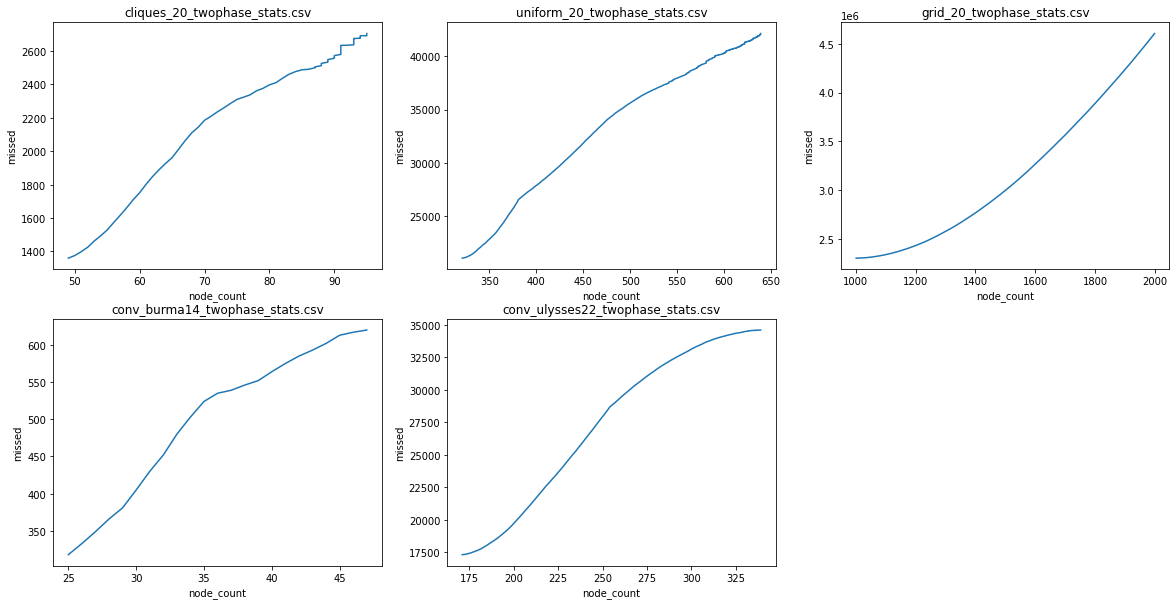
\includegraphics[width=\textwidth]{chapters/experiments/img/merged_plots/per1_all/missed.png}
    \caption{Liczba nieudanych prób tworzenia krawędzi w zależności od liczby wierzchołków --- próbkowanie dwufazowe}
    \label{fig:small_missed}
\end{figure}


Zależność liczby krawędzi od liczby wierzchołków jest nieliniowa dla wszystkich zbadanych instancji i obu algorytmów (rys. \ref{fig:small_edge_count}, rys. \ref{fig:small_edge_to_node}).
Dla instancji typu grid oraz ulysses22 wykres tej zależności ma postać ''gładkiej'' krzywej.
W pozostałych przypadkach wzrost jest znacznie mniej stabilny - pojawiają się ''schodki'', miejsca w których wzrost
spowalnia i gwałtownie rośnie.
Sugeruje to, że przewidzenie wartości stosunku krawędzi do wierzchołków może być możliwy w przypadku
instancji z miastami ułożonymi na siatce.

W przypadku metryki assortativity\_deg można zaobserwować pewną właściwość.
Na początku próbkowania wartość metryki zmienia się gwałtownie, zwiększając i zmniejszając się naprzemiennie (rys. \ref{fig:small_assortativity_deg}).
Po pewnym czasie jednak się stabilizuje, widoczne jest to zwłaszcza dla instancji z większą ilością optimów lokalnych.
Nadal obecne są wahania wartości, ale są one znacznie mniejsze.
Wyjątkiem jest instancja grid\_20 próbkowana algorytmem snowball.
W tym przypadku wartość zmienia się znacznie przez cały okres próbkowania.
W wielu przypadkach ostatnia uzyskana wartość różni znacznie pomiędzy algorytmami.

W większości przypadków średnia wartość funkcji celu przestrzeni zwiększa się wraz z ilością wierzchołków (rys. \ref{fig:small_avg_fitness}).
W niektórych przypadkach występuje początkowo duża wartość i gwałtowny spadek, zwykle w przypadku próbkowania dwufazowego.
W innych przypadkach wartość wzrasta przez cały czas.
Wykresy wartości uzyskane z obu algorytmów różnią się, ale wartości uzyskane na końcu próbkowania są do siebie podobne.
Niska wartość funkcji celu na początku i powolny wzrost oznacza, że w badanych instancjach szybko znajdowane były
najlepsze rozwiązania w przestrzeni.

Wartość współczynnika conrel jest nieprzewidywalna (rys. \ref{fig:small_conrel}).
Dla niektórych instancji utrzymuje się na podobnym poziomie przez większość czasu,
ale gwałtownie zwiększa się pod koniec próbkowania.
W innych wartość miary znacznie zmienia się w trakcie procesu, formując ostre piki.

Gęstość grafu w każdym przypadku osiągała wysoką wartość, by następnie gwałtownie spaść i ustabilizować się w pewnym zakresie (rys. \ref{fig:small_density}).
W kilku przypadkach występował wzrost gęstości grafu pod koniec próbkowania.
Miara jest najbardziej stabilna dla instancji z miastami rozłożonymi równomiernie.

Miara distLO jest niestabilna, występują częste nagłe wzrosty i spadki jej wartości (rys. \ref{fig:small_distLO}).
W kilku przypadkach wystąpił duży spadek pod koniec próbkowania, w innych - gwałtowny wzrost.

Współczynnik wzajemności (reciprocity) również jest niestabilny (rys. \ref{fig:small_reciprocity}).
W niektórych przypadkach występuje gwałtowny wzrost i spadek wartości na początku próbkowania.
Ciekawa jest instancja grid\_20 - po spróbkowaniu odpowiednio dużej liczby wierzchołków
wartość wzrost tej miary jest zbliżony do wzrostu liniowego.

Rozmiar największej kliki zmienia się ''schodkowo'' w momencie, w którym albo ze spróbkowanych wierzchołków
powstanie większa klika lub nowy wierzchołek zostanie odnaleziony w już istniejącej (rys. \ref{fig:small_largest_clique_size}).
Wyniki sugerują że możliwe jest oszacowanie wielkości największej kliki przestrzeni na podstawie wartości
z krótszego próbkowania, zwłaszcza na podstawie danych z próbkowania dwufazowego, gdzie
wartość zmienia się mniej gwałtownie. Ze względu na stopniowy i nieliniowy charakter wzrostu zmiennej,
dokładność takiego szacowania nie będzie duża.

Liczba źródeł, ścieków i tzw. subsinks w grafie w wielu przypadkach początkowo rośnie, by nagle zmaleć na końcu próbkowania.
W przypadkach ze zbioru TSPLIB po pewnym czasie liczba ścieków i subsinks przestała się zmieniać.
Wszystkie trzy miary są niestabilne, mają charakter nieprzewidywalny (rys. \ref{fig:small_num_sinks}, rys. \ref{fig:small_num_sources}, rys. \ref{fig:small_num_subsinks}).

Charakterystyka wzrostu wartości średniego stopnia wchodzącego wierzchołka jest bardziej zbliżona do liniowej
w przypadku próbkowania dwufazowego. W instancjach cliques\_20, uniform\_20 i burma14 występuje
wzrost przyspieszenie wzrostu pod koniec próbkowania (rys. \ref{fig:small_avg_in_degree}).
W tych przypadkach z dużym prawdopodobieństwem algorytmy znalazły wszystkie optima lokalne.
Może być to powodem tego zjawiska.
W przypadku instancji grid\_20 o liczbie optimów lokalnych znacznie wyższej od pozostałych instancji tego rozmiaru,
wynik z próbkowania snowball ma charakter eksponencjalny.
Podobnie wyglądają miary największego stopnia wchodzącego, średniego stopnia wychodzącego i maksymalnego stopnia wychodzącego
(rys. \ref{fig:small_max_in_degree}, rys. \ref{fig:small_avg_out_degree}, rys \ref{fig:small_max_out_degree}).

Średnia waga pętli w grafie jest niestabilna, w niektórych przypadkach wzrost jest bliski liniowego, w innych
eksponencjalnego, a w pozostałych jest chaotyczny (rys. \ref{fig:small_avg_loop_weight}).

Średnia długość ścieżki w grafie zwiększa się gwałtownie na początku, po czym stabilizuje (rys. \ref{fig:small_avg_path_len}).
Pojawiają się przypadki odstające (w grid\_20 przy próbkowaniu snowball wartość dość szybko maleje),
ale dla większości przypadków wahania wartości po ustabilizowaniu są niewielkie.
Podobnie jest w przypadku średniej długości ścieżek do globalnego optimum.

Długość najdłuższej ścieżki do globalnego optimum zmniejsza i zwiększa się gwałtownie.
Jest nieprzewidywalna, podobnie jest z wartością maksymalną (rys. \ref{fig:small_avg_go_path_len}, rys. \ref{fig:small_max_go_path_len}).

Współczynnik go\_path\_ratio zmienia się zupełnie inaczej w zależności od algorytmu próbkowania (rys. \ref{fig:small_go_path_ratio}).
Próbkowanie dwufazowe rośnie gwałtownie i bardzo wcześnie się stabilizuje.
Próbkowanie snowball prowadzi natomiast do powolnego wzrostu z okazjonalnymi spadkami wartości.
Oba algorytmy osiągają podobną końcową wartość miary, ale próbkowanie dwufazowe osiąga ją przy mniejszej
liczbie spróbkowanych wierzchołków.

Liczba lejów w przestrzeni jest miarą niestabilną, wartość miary zmienia się w zupełnie inny sposób
dla różnych instancji (rys. \ref{fig:small_funnel_num}).

Rozmiar największego leja w przestrzeni rośnie liniowo dla danych uzyskanych z próbkowania
dwufazowego. Wartość uzyskana z próbkowania snowball nie jest tak stabilna (rys. \ref{fig:small_max_funnel_size}).

Wzrost średniego rozmiaru lejów dla próbkowania dwufazowego również jest bliski liniowego,
widać jednak na nim pewne odchylenia (rys. \ref{fig:small_mean_funnel_size}). W ramach wzrostu ilości optimów lokalnych w przestrzeni,
wykres uzyskany ze snowball coraz bardziej zbliża się do wzrostu eksponencjalnego.

Liczba spójnych podgrafów szybko stabilizuje się na stałej wartości dla większości przypadków (rys. \ref{fig:small_num_cc}).

Rozmiar największego spójnego podgrafu rośnie liniowo dla wszystkich instancji i algorytmów (rys. \ref{fig:small_largest_cc}).

Promień największego spójnego podgrafu zmienia się wielokrotnie o wartość 1 dla większości przypadków (rys. \ref{fig:small_largest_cc_radius}).

Im więcej wierzchołków znajduje się w zbiorze, tym więcej prób tworzenia krawędzi w algorytmie dwufazowym
się powiedzie. Dlatego można zaobserwować delikatne wypłaszczenie krzywej na wykresie liczby nieudanych prób.
Wyjątkiem jest tu instancja grid\_20  - jest to spowodowane tym że algorytm nie znalazł wszystkich optimów
lokalnych przed końcem próbkowania (rys. \ref{fig:small_missed}).

\newpage

\subsection{Badanie stabilności dla dużych instancji}
W tej sekcji opisano badania przeprowadzone dla instancji o rozmiarze 48 i większym.

Próbkowanie algorytmem snowball wykonano z następującymi parametrami:
\begin{itemize}
    \item $w_{len}$ - długość losowego spaceru - 10000
    \item $m$ - liczba prób przeszukania sąsiedztwa - 100
    \item $depth$ - głębokość przeszukiwania - 3
\end{itemize}

Próbkowanie algorytmem \textit{snowball} prowadzono do zakończenia losowego spaceru lub osiągnięcia liczby 100000 wierzchołków.
Dla instancji \textbf{cliques\_50} z powodu małej liczby optimów lokalnych zapis wykonywano co 100 znalezionych wierzchołków.
Dla pozostałych instancji stan próbkowania zapisywany był co 1000 znalezionych wierzchołków.

Próbkowanie algorytmem dwufazowym przeprowadzono z następującymi parametrami:
\begin{itemize}
    \item $n_{max}$ - żądana liczba wierzchołków - 1000
    \item $n_{att}$ - liczba prób generowania wierzchołków - 1000
    \item $e_{att}$ - liczba prób generowania krawędzi - 1000
    \item $n_{runs}$ - liczba powtórzeń - 100
\end{itemize}

Próbkowanie przeprowadzono przez ustaloną z góry liczbę powtórzeń, zapisując stan przestrzeni po zakończeniu każdego powtórzenia.

Po zakończeniu próbkowania dla każdego zapisanego stanu przestrzeni obliczono wartości badanych miar. W ten sposób uzyskano
wartości miar dla różnych etapów próbkowania przestrzeni.

Utworzono wykresy przedstawiające zależność wartości miar od liczby spróbkowanych wierzchołków.
Przedstawiono je na rysunkach od \ref{fig:main_snowball_edge_count} do \ref{fig:main_twophase_missed}.

Ze względu na długi czas obliczeń i ograniczony czas realizacji projektu,
dla instancji cliques\_50, cliques\_80, uniform\_50, att48, berlin52 i pr76 i próbkowania dwufazowego
nie wykonano obliczeń wartości następujących miar:

\begin{itemize}
    \item num\_subsinks
    \item num\_cc
    \item largest\_cc
    \item largest\_cc\_radius
    \item avg\_path\_len
    \item largest\_clique\_size
    \item reciprocity
\end{itemize}

\subsubsection{Wyniki}

\foreach \metric/\cap in \metrics{
    \begin{figure}[p]
        \centering
        \includegraphics[width=\textwidth]{chapters/experiments/img/merged_plots/main_snowball/\metric.png}
        \caption{\cap \space w zależności od liczby wierzchołków - próbkowanie snowball}
        \label{fig:main_snowball_\metric}
    \end{figure}
}

\newpage

\foreach \metric/\cap in \metrics{
    \begin{figure}[p]
        \centering
        \includegraphics[width=\textwidth]{chapters/experiments/img/merged_plots/main_twophase/\metric.png}
        \caption{\cap \space w zależności od liczby wierzchołków - próbkowanie dwufazowe}
        \label{fig:main_twophase_\metric}
    \end{figure}
}

\begin{figure}[h!]
    \centering
    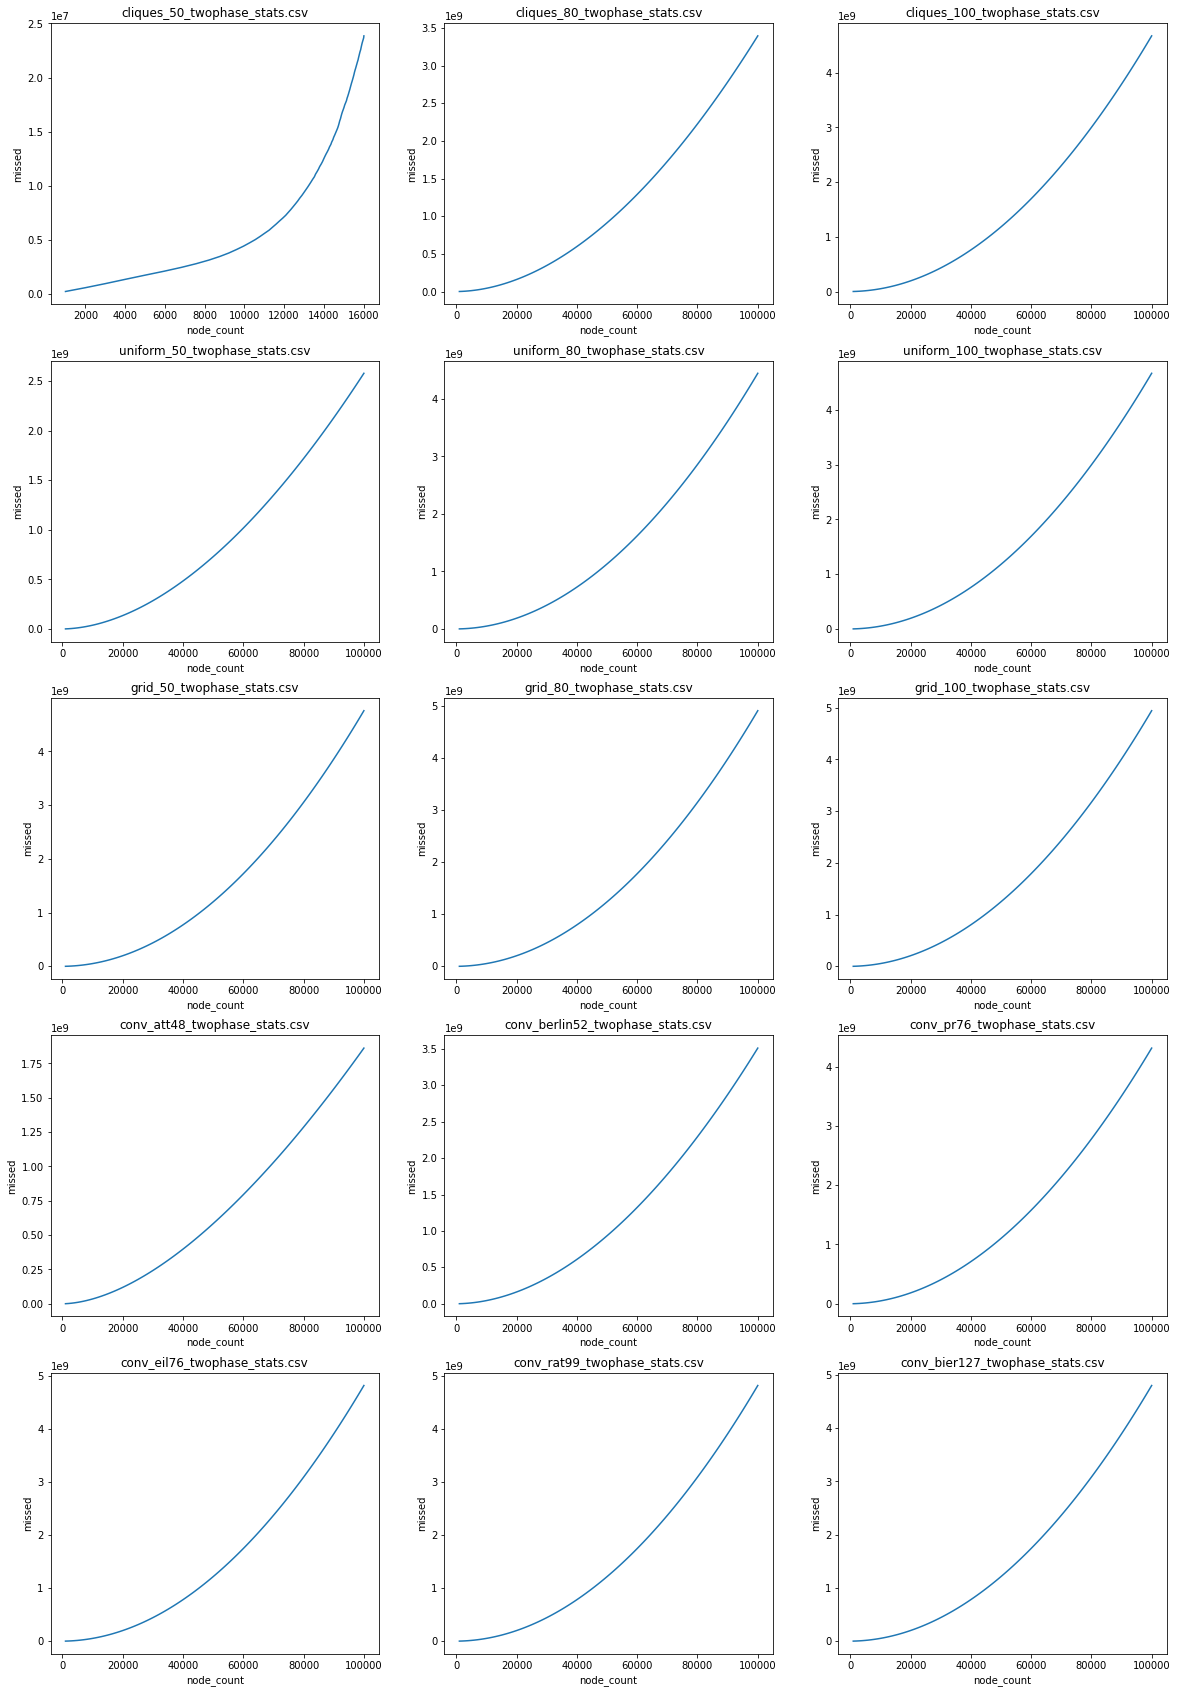
\includegraphics[width=\textwidth]{chapters/experiments/img/merged_plots/main_twophase/missed.png}
    \caption{Liczba nieudanych prób tworzenia krawędzi w zależności od liczby wierzchołków - próbkowanie dwufazowe}
    \label{fig:main_twophase_missed}
\end{figure}

\begin{figure}[h!]
    \centering
    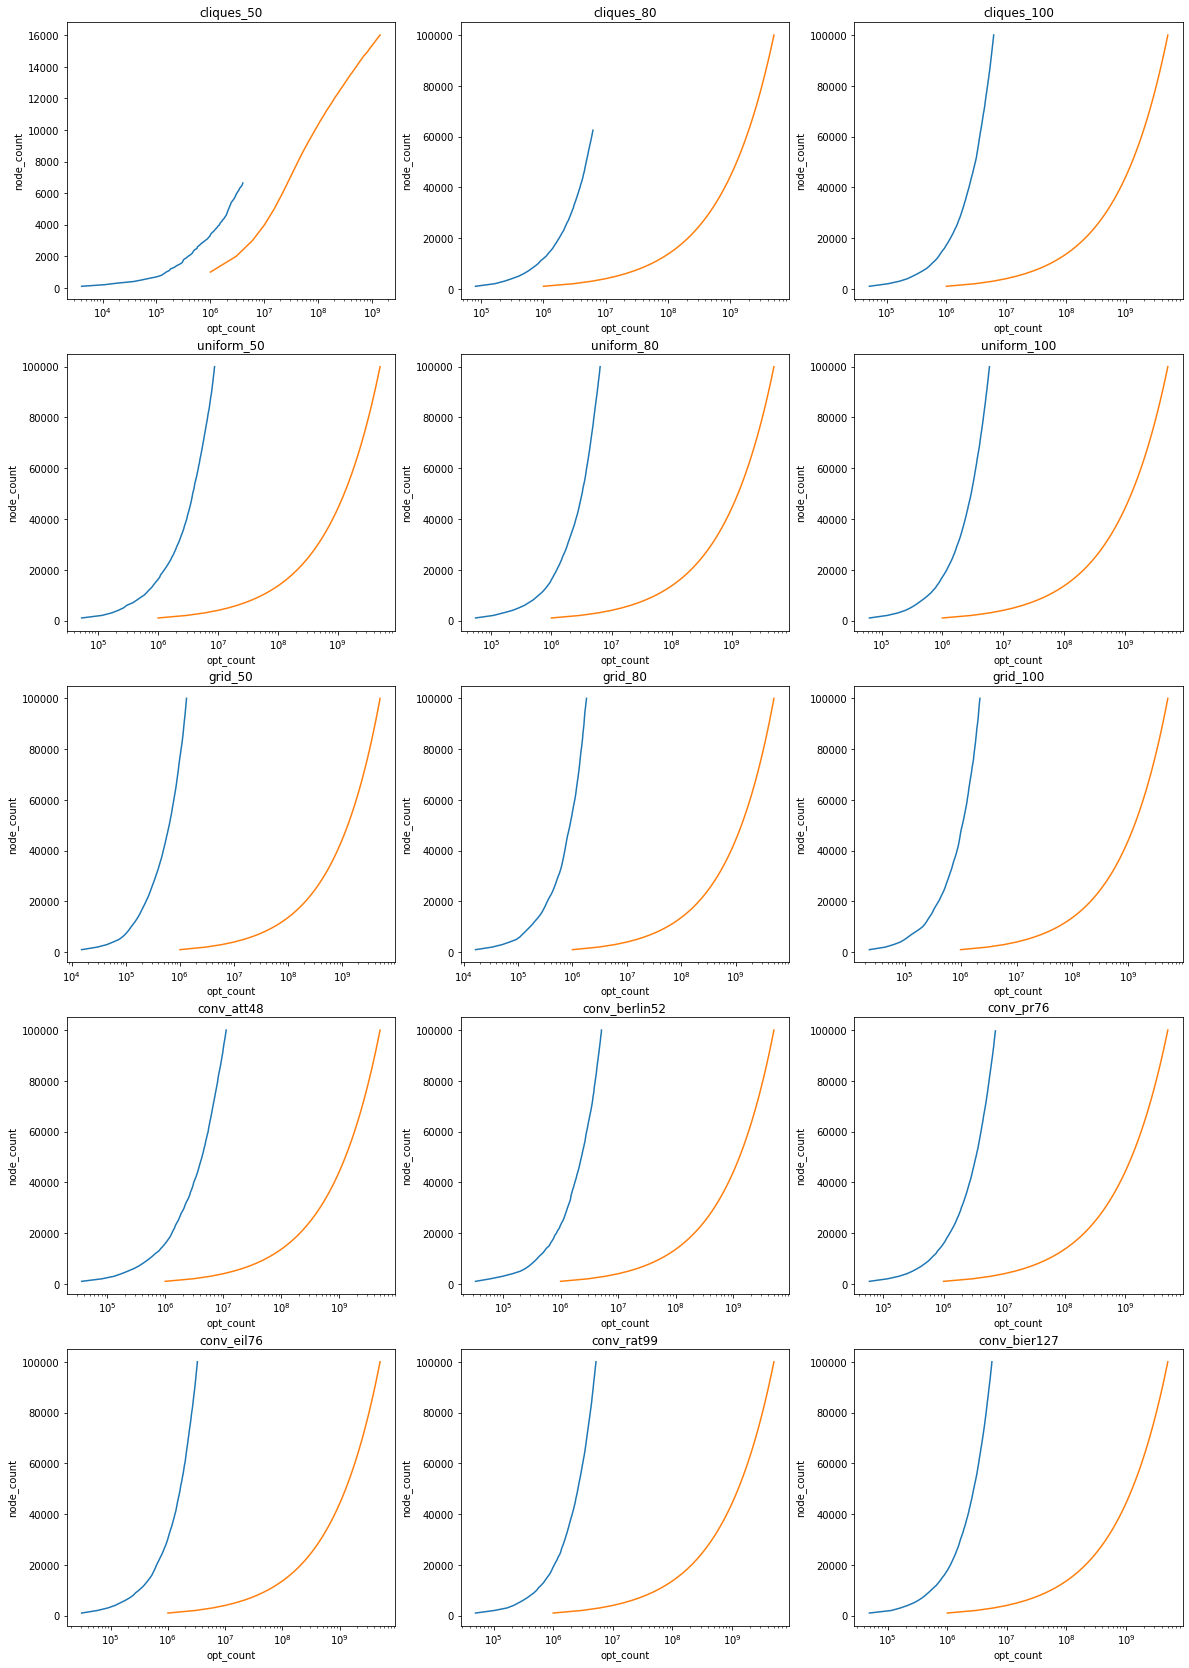
\includegraphics[width=\textwidth]{chapters/experiments/img/opt_nodes.png}
    \caption{Wykres zależności liczby wierzchołków od liczby wywołań funkcji celu.
        Kolor niebieski - próbkowanie snowball, kolor pomarańczowy - próbkowanie dwufazowe.
        Oś X w skali logarytmicznej}
    \label{fig:main_opt_nodes}
\end{figure}

\begin{figure}[h!]
    \centering
    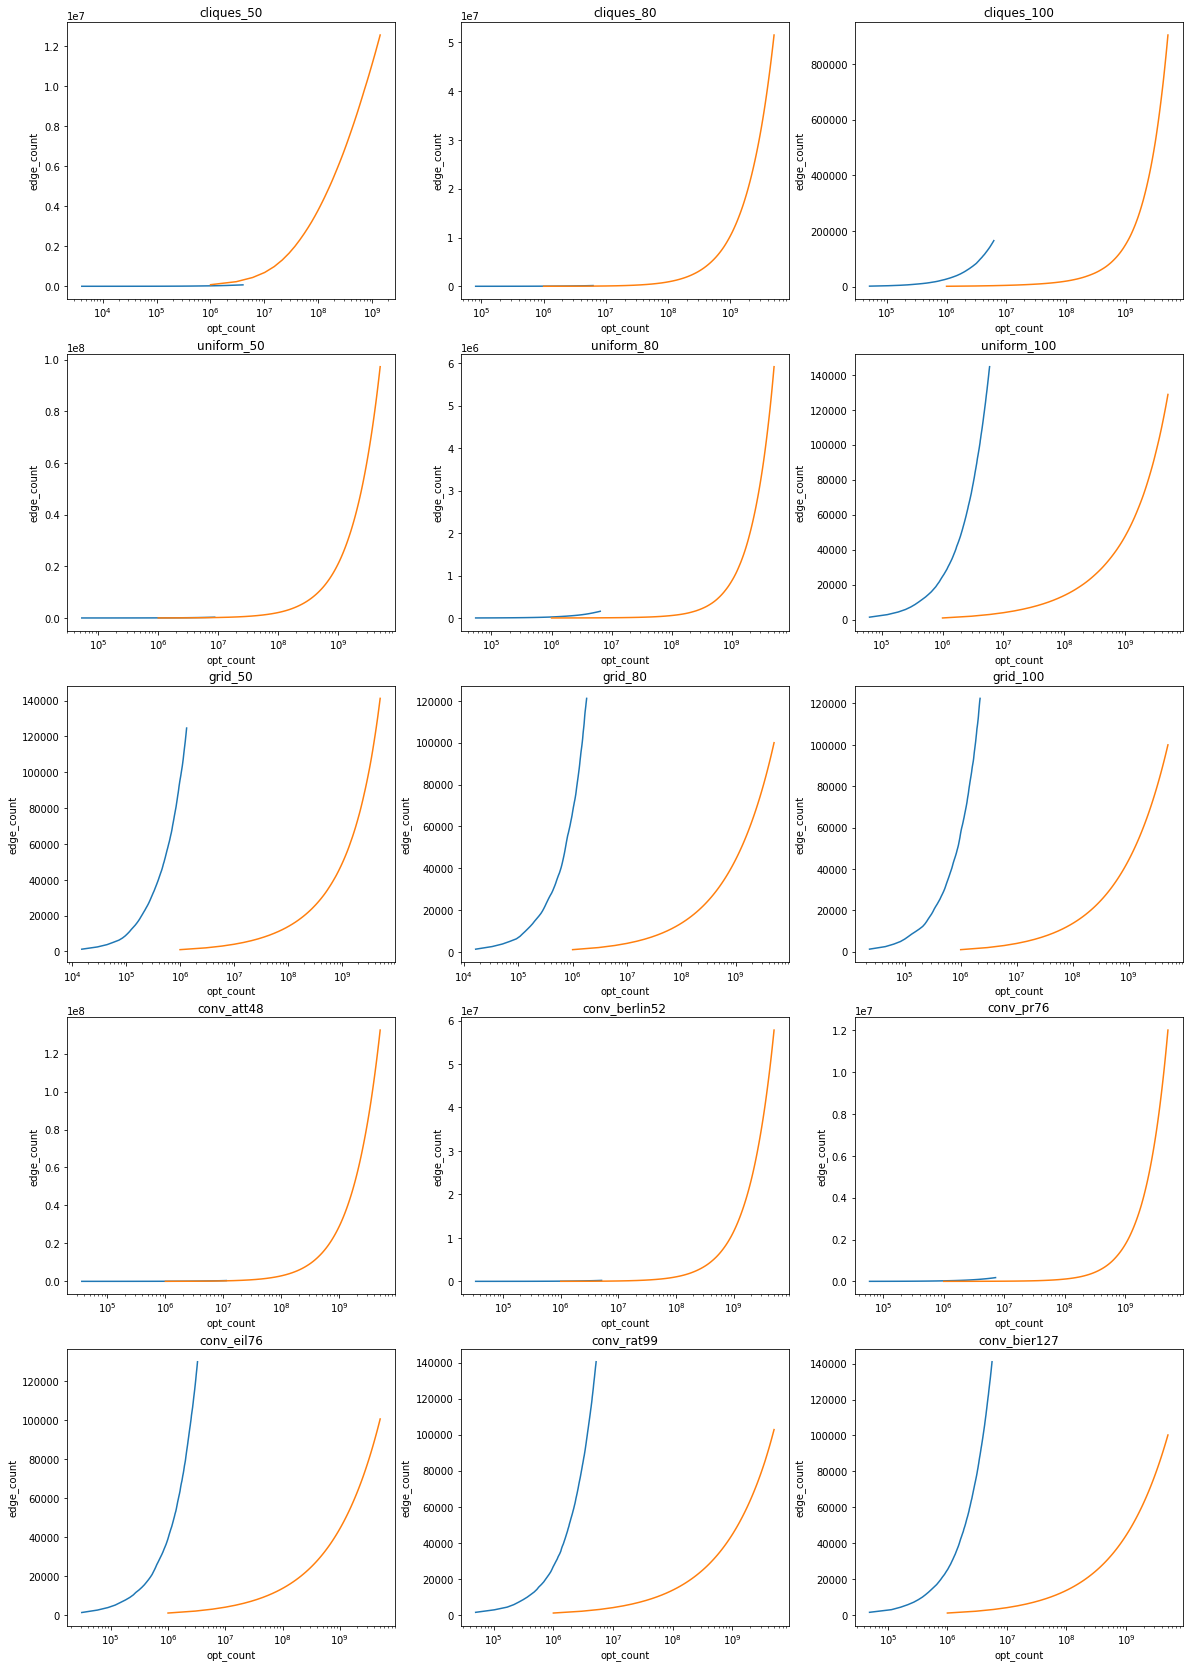
\includegraphics[width=\textwidth]{chapters/experiments/img/opt_edges.png}
    \caption{Wykres zależności liczby krawędzi od liczby wywołań funkcji celu.
        Kolor niebieski - próbkowanie snowball, kolor pomarańczowy - próbkowanie dwufazowe.
        Oś X w skali logarytmicznej}
    \label{fig:main_opt_edges}
\end{figure}




Wzrost liczby krawędzi w stosunku do liczby wierzchołków jest zbliżony do liniowego dla próbkowania snowball (rys. \ref{fig:main_snowball_edge_count}).
Na wykresie wartości stosunku krawędzi do wierzchołków (rys. \ref{fig:main_snowball_edge_to_node}), w niektórych przypadkach widać co prawda gwałtowne zmiany, ale
ich bezwzględna wartość jest niewielka.
W przypadku próbkowania dwufazowego (rys. \ref{fig:main_twophase_edge_count}, rys.\ref{fig:main_twophase_edge_to_node}), ta zależność nie jest liniowa dla części instancji,
najlepiej widać to w przypadku instancji cliques\_50, cliques\_80, att48, berlin52, oraz pr76.
Dla instancji typu grid oraz pozostałych instancji ze zbioru tsplib zależność ma charakterystykę liniową lub zbliżoną do liniowej.

Współczynnik różnorodności grafu nie jest stabilny. Wykres jego wartości wygląda inaczej w niemal każdym przypadku
próbkowania snowball (rys. \ref{fig:main_snowball_assortativity_deg}).
Dla próbkowania dwufazowego (rys. \ref{fig:main_twophase_assortativity_deg}) można zaobserwować eksponencjalny spadek wartości taj miary dla części instancji.
W innych przypadkach wzrasta ona szybko i oscyluje wokół pewnej wartości.
Odstającym przypadkiem są instancje grid\_80 i grid\_100. Wykres pokazuje dla nich stałą wartość 0.
W rzeczywistości otrzymano tutaj wartość nieprawidłową (NaN). Najprawdopodobniej mianownik wyrażenia \ref{eq:assortativity}
miał wartość 0.

Dla większości instancji o rozmiarze 50 średnia wartość funkcji celu jest niska na początku i wzrasta podczas dalszego próbkowania.
Zależność tą możemy zaobserwować zarówno w przypadku próbkowania snowball jak i dwufazowego (rys. \ref{fig:main_snowball_avg_fitness}, rys. \ref{fig:main_twophase_avg_fitness}).
W przypadku instancji większych oraz typu grid po początkowym spadku wartości, maleje ona dalej lub stabilizuje się na pewnym poziomie.
Nie jest to zaskakujące. W mniejszych instancjach problemu występuje mniej lokalnych optimów, więc zwiększa się szansa, że algorytm
natrafi na nie podczas krótszego próbkowania. Instancje większe zawierają znacznie więcej optimów lokalnych, więc nawet po długim próbkowaniu
algorytm wciąż natrafia na nowe o niższej wartości funkcji celu. Instancje typu grid charakteryzują się dużą liczbą optimów lokalnych,
więc problem ten występuje również dla mniejszych instancji tego typu.

Wartość współczynnika conrel jest niestabilna. Różni się ona w zależności od algorytmu próbkowania (rys. \ref{fig:main_snowball_conrel}, rys. \ref{fig:main_twophase_conrel}).
Dla większych instancji typu grid i próbkowania dwufazowego ma ona stałą wartość 0.

Wartość gęstości grafu (density) zmienia się w przewidywalny sposób dla próbkowania snowball (rys. \ref{fig:main_snowball_density}) i maleje eksponencjalnie.
W przypadku próbkowania dwufazowego (rys. \ref{fig:main_twophase_density}) taki spadek występuje tylko w instancjach typu grid, instancji cliques\_100 oraz większych
instancjach ze zbioru tsplib.
Dla pozostałych instancji występują kolejne wzrosty i spadki wartości tej miary.
Z otrzymanych danych można wywnioskować, że wartość tej metryki jest w dużym stopniu zależna od wykorzystanego algorytmu próbkowania.

Wartość współczynnika distLO jest niestabilna. Zmienia się w nieprzewidywalny sposób zarówno dla algorytmu snowball jak i dwufazowego (rys. \ref{fig:main_snowball_distLO}, rys. \ref{fig:main_twophase_distLO}).
Ciekawym przypadkiem są instancje grid dla próbkowania snowball - wartość distLO jest dla nich stała i wynosi 1. Oznacza to, że każda krawędź połączona
z najlepszym rozwiązaniem miała wagę 1 przez cały okres próbkowania.

Wzajemność grafu (reciprocity) w większości przypadkach gwałtownie zmienia się na początku, a potem stabilizuje w okolicach pewnej wartości.
W przypadku instancji grid\_80 i grid\_100 otrzymano wartości nieprawidłowe (NaN) dla całego okresu próbkowania dwufazowego (rys. \ref{fig:main_twophase_reciprocity}). W rzeczywistości oznacza to
najprawdopodobniej, że wszystkie krawędzie mają swojego przeciwnego odpowiednika - mianownik wyrażenia \ref{eq:reciprocity} zeruje się, gdy w grafie nie występuje ani jedna krawędź,
której nie odpowiada krawędź w kierunku przeciwnym. Podobne nieprawidłowe wartości występują również na początku próbkowania dużych instancji rzeczywistych.
Jest to najprawdopodobniej spowodowane działaniem algorytmu próbkowania. Na początku wiele optimów lokalnych nie znajduje się w zbiorze wierzchołków.
Z tego powodu nie udaje się utworzyć dużej ilości krawędzi prowadzących do nieodkrytych jeszcze wierzchołków.
Jeśli już uda się utworzyć krawędź, to z dużym prawdopodobieństwem algorytm spróbkuje również krawędź w przeciwnym kierunku.
Im większa przestrzeń przeszukiwania, tym dłużej będzie występował ten problem.
Zjawisko to nie występuje dla algorytmu snowball, gdyż tam wierzchołki są próbkowane równocześnie z krawędziami i każda krawędź, która może powstać jest
tworzona od razu (rys. \ref{fig:main_snowball_reciprocity}) .

Rozmiar największej kliki w grafie wzrasta ''schodkowo'' dla obu algorytmów (rys. \ref{fig:main_snowball_largest_clique_size}, (rys. \ref{fig:main_twophase_largest_clique_size})).
Dla największych instancji jego wartość nie zmienia się przez cały okres próbkowania.
Z danych można wywnioskować, że im mniejsza ilość lokalnych optimów w przestrzeni przeszukiwania, tym częściej zmienia się wartość tej miary.
Stała wartość dla dużych instancji nie oznacza, że można ją przyjąć za wartość miary dla całej przestrzeni - najprawdopodobniej zmieni się
ona po jeszcze dłuższym próbkowaniu.

Liczba źródeł w grafie rośnie liniowo dla większości instancji przy próbkowaniu snowball (rys. \ref{fig:main_snowball_num_sources}).
W przypadku próbkowania dwufazowego zależność liniowa występuje jedynie w przypadku największych instancji i instancji typu grid (rys. \ref{fig:main_twophase_num_sources}).
Ciekawym przypadkiem jest instancja cliques\_50, w której jako jedynej wartość tej miary zaczyna spadać pod koniec próbkowania.

Liczba ścieków w grafie również rośnie liniowo dla większości instancji w przypadku próbkowania snowball (rys. \ref{fig:main_snowball_num_sinks}).
W przypadku próbkowania dwufazowego jest zupełnie inaczej. O ile liniowy wzrost wciąż występuje dla niektórych instancji, to w innych przypadkach
wartość ta maleje lub utrzymuje się na stałym poziomie. Instancja cliques\_50 również się tu wyróżnia - w przestrzeni rozwiązań występują jedynie dwa ścieki
przez cały okres próbkowania (rys. \ref{fig:main_twophase_num_sinks}).
Wykresy ilości subsinks wyglądają niemal identycznie do wykresów ilości ścieków - oznacza to, że ich liczba jest zawsze zbliżona
(rys. \ref{fig:main_snowball_num_subsinks}, rys. \ref{fig:main_twophase_num_subsinks}).

Średni stopień wchodzący wierzchołków jest miarą nieprzewidywalną dla próbkowania snowball (rys. \ref{fig:main_snowball_avg_in_degree}).
W przypadku próbkowania dwufazowego wartość miary jest bardziej przewidywalna - przez cały czas wzrasta dla większości przypadków (rys. \ref{fig:main_twophase_avg_in_degree}).
Wyjątkiem są instancje grid\_80 i grid\_100, w których przez cały okres próbkowania otrzymywana jest wartość 0.
Maksymalny stopień wchodzący dla części instancji wzrasta ''schodkowo'', a dla innych łagodniej (rys. \ref{fig:main_snowball_max_in_degree}, rys. \ref{fig:main_twophase_max_in_degree}).
W przypadku algorytmu dwufazowego dla niektórych instancji wzrost jest bliski liniowego.
Instancje grid\_80 i grid\_100 mają maksymalny stopień wchodzący równy 0.
Oznacza to, że wszystkie krawędzie w tych grafach to pętle. Wyjaśnia to również wartość distLO równą 1.
Podobnie prezentują się wykresy wartości średniej i maksymalnej stopnia wychodzącego
(rys. \ref{fig:main_snowball_avg_out_degree}, rys. \ref{fig:main_snowball_max_out_degree}, rys. \ref{fig:main_twophase_avg_out_degree}, rys. \ref{fig:main_twophase_max_out_degree}).

Średnia waga pętli w grafie jest nieprzewidywalna dla próbkowania snowball (rys. \ref{fig:main_snowball_avg_loop_weight}, rys. \ref{fig:main_twophase_avg_loop_weight}).
Dla próbkowania dwufazowego wielkość ta wzrasta niemal liniowo dla każdej instancji oprócz cliques\_50.

Średnia długość ścieżki w grafie jest nieprzewidywalna dla większości instancji próbkowanych algorytmem snowball (rys. \ref{fig:main_snowball_avg_path_len}).
Wyjątkiem są instancje typu grid, dla których wartość tej metryki stale wzrasta.
Dla próbkowania dwufazowego również nie uzyskano stabilnych wartości.
Pętle nie są brane pod uwagę w obliczaniu wartości tej metryki. Z tego powodu wynosi ona 0 dla większych instancji typu grid (rys. \ref{fig:main_twophase_avg_path_len}).

Średnia długość ścieżki do najlepszego rozwiązania jest nieprzewidywalna niezależnie od algorytmu próbkującego (rys. \ref{fig:main_snowball_avg_go_path_len}, rys. \ref{fig:main_twophase_avg_go_path_len}).
Nagłe zmiany w wartości są spowodowane najprawdopodobniej znalezieniem nowego najlepszego rozwiązania w przestrzeni.
Podobnie jest w przypadku wartości maksymalnej (rys. \ref{fig:main_snowball_max_go_path_len}, rys. \ref{fig:main_twophase_max_go_path_len}).

Współczynnik go\_path\_ratio jest nieprzewidywalny. O ile w niektórych przypadkach przy próbkowaniu dwufazowym stabilizuje się na pewnej wartości
po początkowym wzroście, to w innych gwałtownie zmniejsza się i zwiększa (rys. \ref{fig:main_snowball_go_path_ratio}, rys. \ref{fig:main_twophase_go_path_ratio}).

Dla próbkowania snowball liczba lejów w przestrzeni wzrasta liniowo dla wszystkich instancji oprócz cliques\_50 (rys. \ref{fig:main_snowball_funnel_num}).
Inaczej jest w przypadku próbkowania dwufazowego - tutaj zależność ta wygląda zupełnie inaczej dla różnych instancji.
Liniowy wzrost obserwujemy jedynie w instancjach: eil76, rat99, bier127, grid\_80, grid\_100. Podobnie wyglądają również uniform\_100 i grid\_50.
Dla instancji cliques\_50 wartość miary jest stała przez cały okres próbkowania. W przypadku instancji uniform\_50, att48 i berlin52 wartość miary
szybko zmniejsza się na początku, po czym utrzymuje stałą wartość do końca próbkowania (rys. \ref{fig:main_twophase_funnel_num}).

Rozmiar największego leja dla niektórych instancji wzrasta liniowo. Dla innych wzrasta ''schodkowo'', a w przypadku instancji grid\_80 i grid\_100 dla
próbkowania dwufazowego - ma stałą wartość 1. Oznacza to, że nie da się dokładnie przewidzieć wartości tej miary. Warto jednak zauważyć, że
''schodkowe'' zwiększanie się wartości tej miary występuje w instancjach o największej liczbie lokalnych optimów.
Widoczne są wyraźne różnice pomiędzy wykresami uzyskanymi z próbkowania snowball i dwufazowego (rys. \ref{fig:main_snowball_max_funnel_size}, rys. \ref{fig:main_twophase_max_funnel_size}).
Nieco inaczej przedstawiają się wykresy średniej wielkości lejów. O ile dla próbkowania snowball wartość zmienia się w sposób całkowicie nieprzewidywalny,
to wszystkie wykresy uzyskane z algorytmu dwufazowego (oprócz grid\_80 i grid\_100) wykazują tendencję wzrostową (choć w niektórych instancjach pojawiają się małe spadki wartości.)
(rys. \ref{fig:main_snowball_mean_funnel_size}, rys. \ref{fig:main_twophase_mean_funnel_size}).

Liczba spójnych podgrafów sieci LON jest stała dla wielu instancji w przypadku próbkowania snowball (rys. \ref{fig:main_snowball_num_cc}). Dla innych zmienia się ona w nieprzewidywalny sposób.
W przypadku próbkowania dwufazowego i instancji grid liczba podgrafów jest równa liczbie wierzchołków, gdyż każdy wierzchołek w tych grafach jest wierzchołkiem izolowanym.
W przypadku instancji ze zbioru tsplib, liczba ta nie jest równa liczbie wierzchołków, ale jest bardzo bliska - oznacza to, że znaczna większość
wierzchołków w tych grafach również jest izolowana (rys. \ref{fig:main_twophase_num_cc}).

W przypadku próbkowania snowball rozmiar największego spójnego podgrafu wzrasta liniowo dla większości instancji. Dla instancji uniform\_100, oraz
eil76, rat99 i bier127 potrafi utrzymywać się na stałym poziomie przez dłuższy czas i nagle rosnąć (rys. \ref{fig:main_snowball_largest_cc}).
W przypadku próbkowania dwufazowego nie wzrasta on liniowo. Dla niektórych instancji wartość utrzymuje się na niskim poziomie przez długi czas (rys. \ref{fig:main_twophase_largest_cc}).
Dla instancji rat99 i bier127 zmienia się częściej niż w przypadku próbkowania snowball.

Promień największego spójnego podgrafu sieci zmienia się w sposób nieprzewidywalny dla obu algorytmów (rys. \ref{fig:main_snowball_largest_cc_radius}, rys. \ref{fig:main_twophase_largest_cc_radius}).

Zależność liczby nieudanych prób tworzenia krawędzi przez algorytm dwufazowy wygląda bardzo podobnie dla wszystkich instancji (rys. \ref{fig:main_twophase_missed}).

Na wykresach \ref{fig:main_opt_nodes} i \ref{fig:main_opt_edges} możemy zobaczyć odpowiednio liczbę wierzchołków i liczbę krawędzi
w zależności od liczby wywołań funkcji optymalizującej. Liczba wywołań funkcji optymalizującej jest zarazem liczbą wywołań funkcji celu, gdyż
algorytm 2opt wykonuje pełną kalkulację długości ścieżki tylko raz.
Na wykresach kolorem niebieskim oznaczono algorytm snowball, a pomarańczowym - algorytm dwufazowy.
Oś X została przedstawiona w skali logarytmicznej.
Na wykresie wyraźnie widać, że spróbkowanie tej samej liczby wierzchołków zawiera o wiele więcej czasu algorytmowi dwufazowemu.
Należy jednak pamiętać, że w niektórych przypadkach (np. cliques\_50 ) szybszy algorytm snowball nie odnalazł wszystkich optimów lokalnych w przestrzeni.
Dla wszystkich instancji cliques, uniform\_50 i uniform\_80, att48, berlin52 oraz pr76 algorytm dwufazowy znalazł również o wiele większą ilość krawędzi.
Co ważne, większość z nich została znaleziona w bardzo późnej fazie próbkowania.

\subsection{Korelacja wzajemna miar}

\begin{figure}[h!]
    \centering
    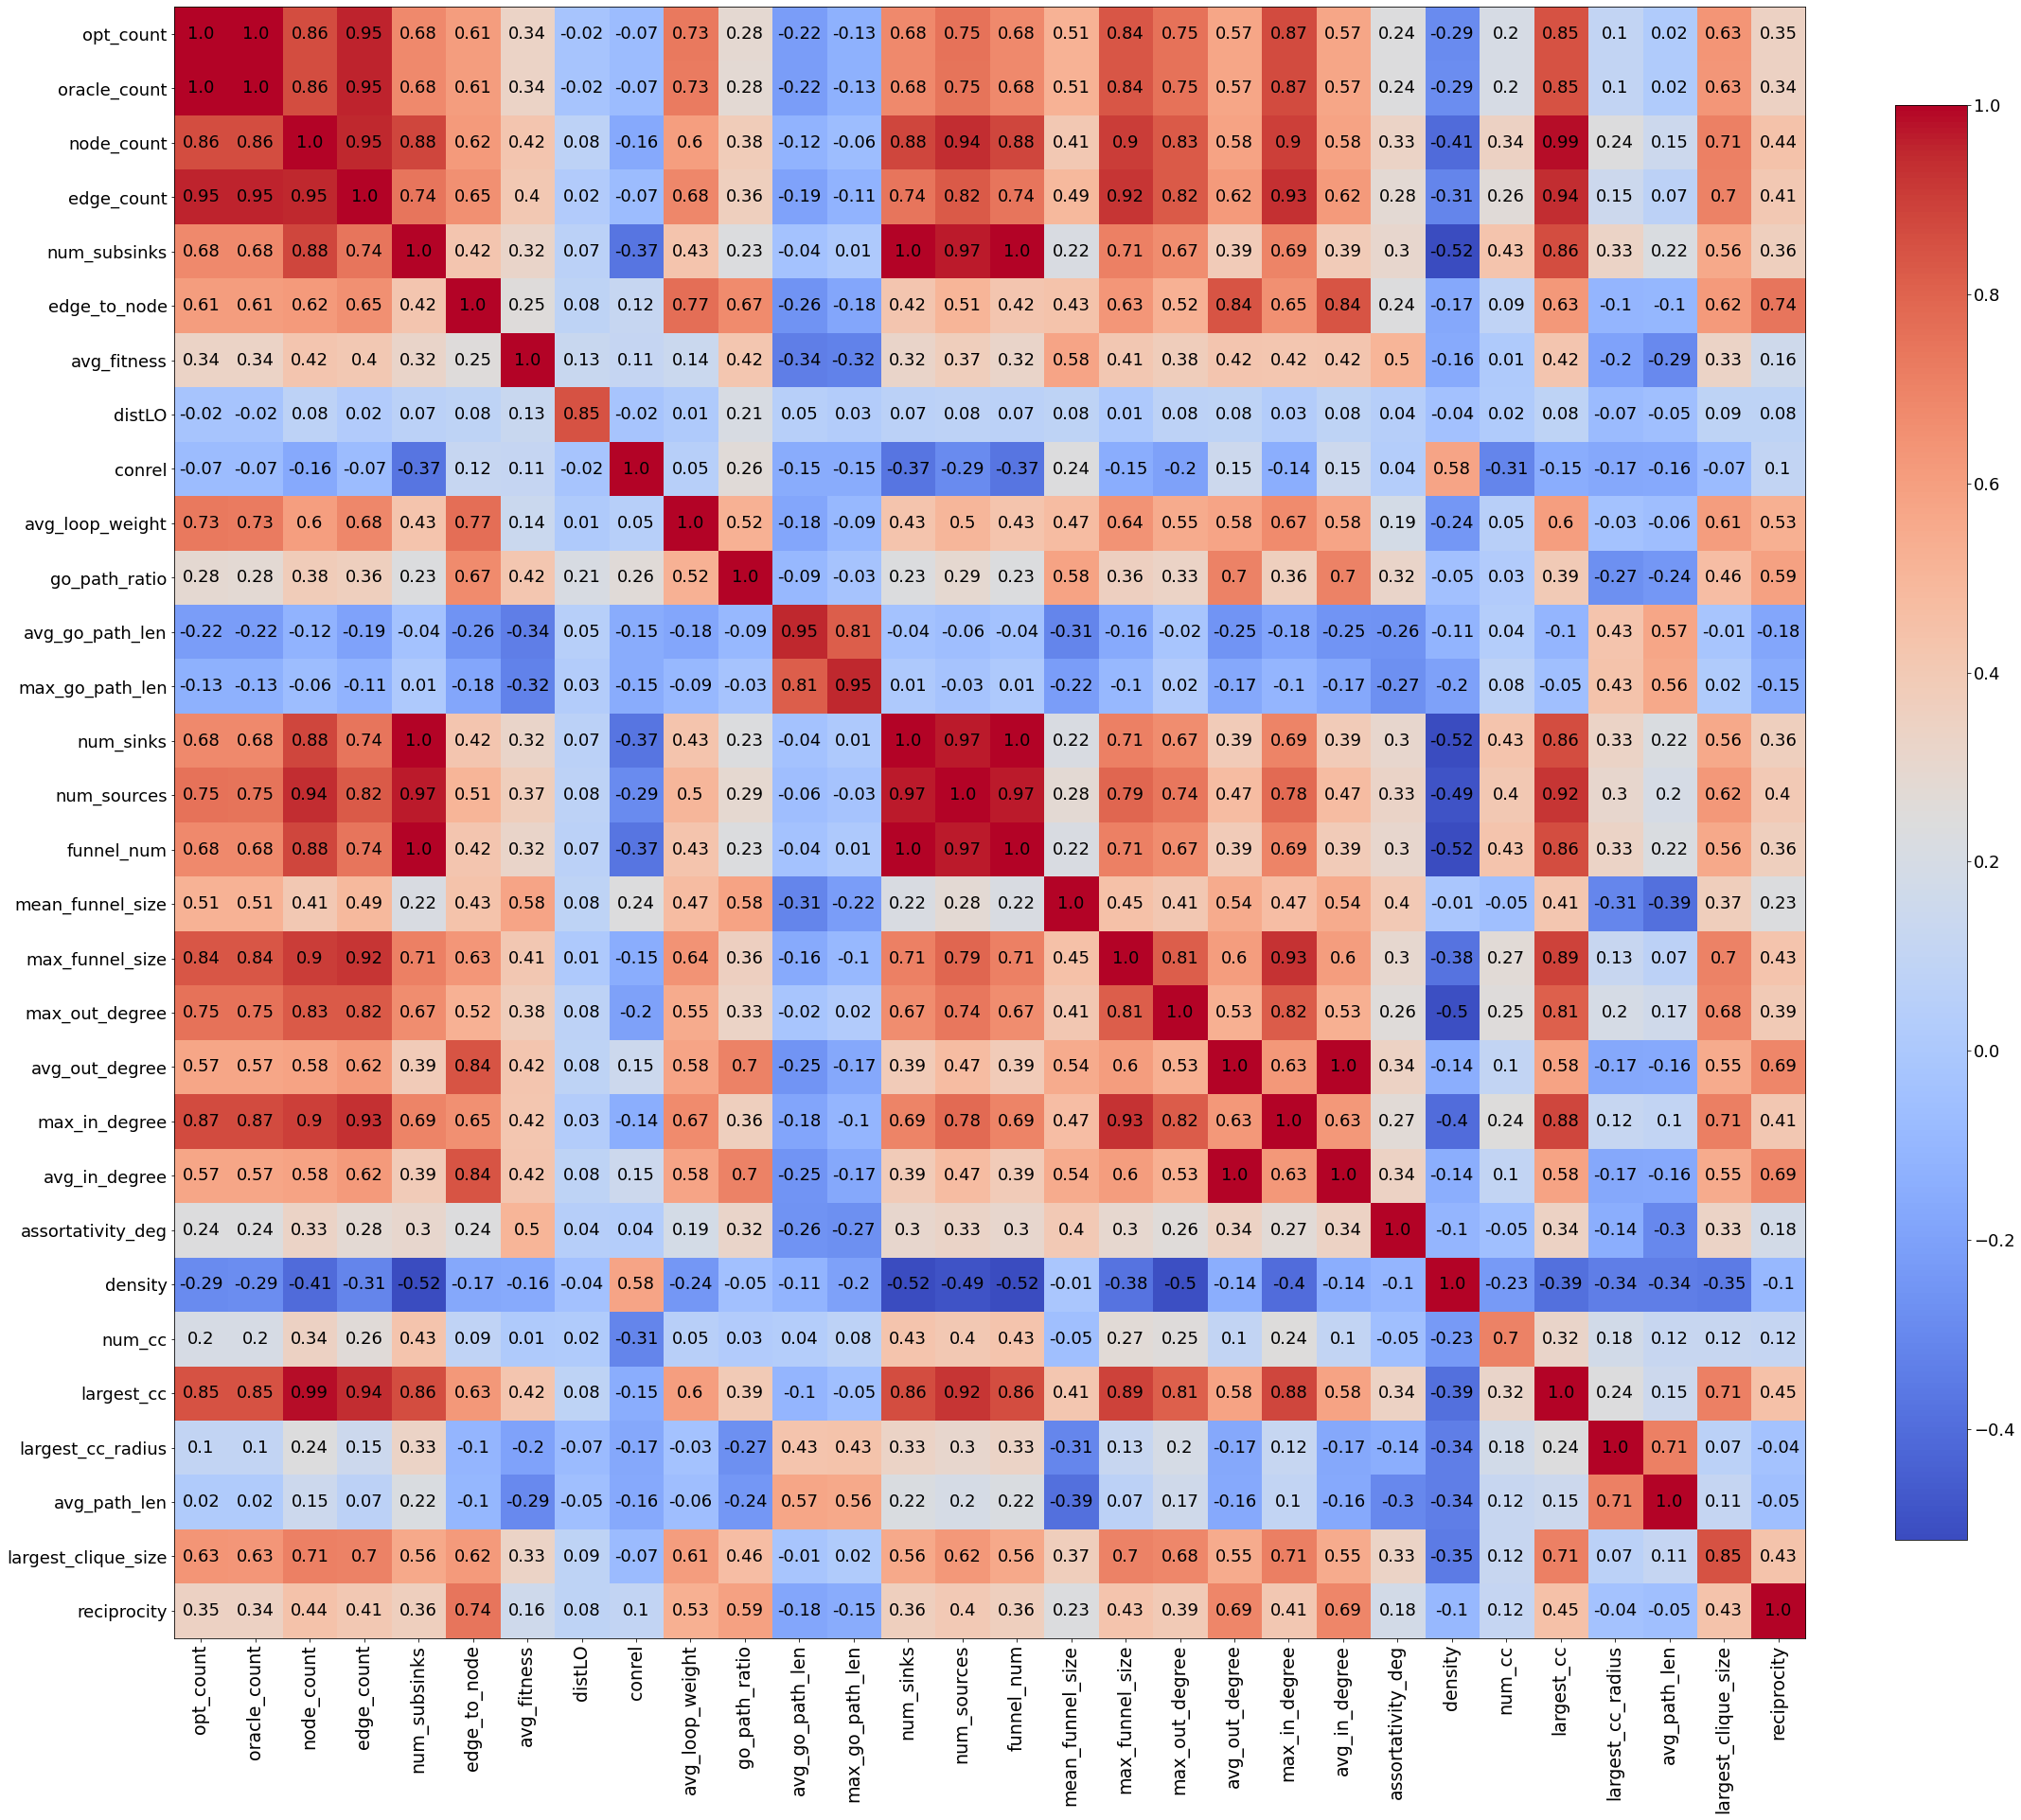
\includegraphics[width=\textwidth]{chapters/experiments/img/snowball_corr.png}
    \caption{Wzajemna korelacja miar - próbkowanie snowball}
    \label{fig:corr_snowball}
\end{figure}

\begin{figure}[h!]
    \centering
    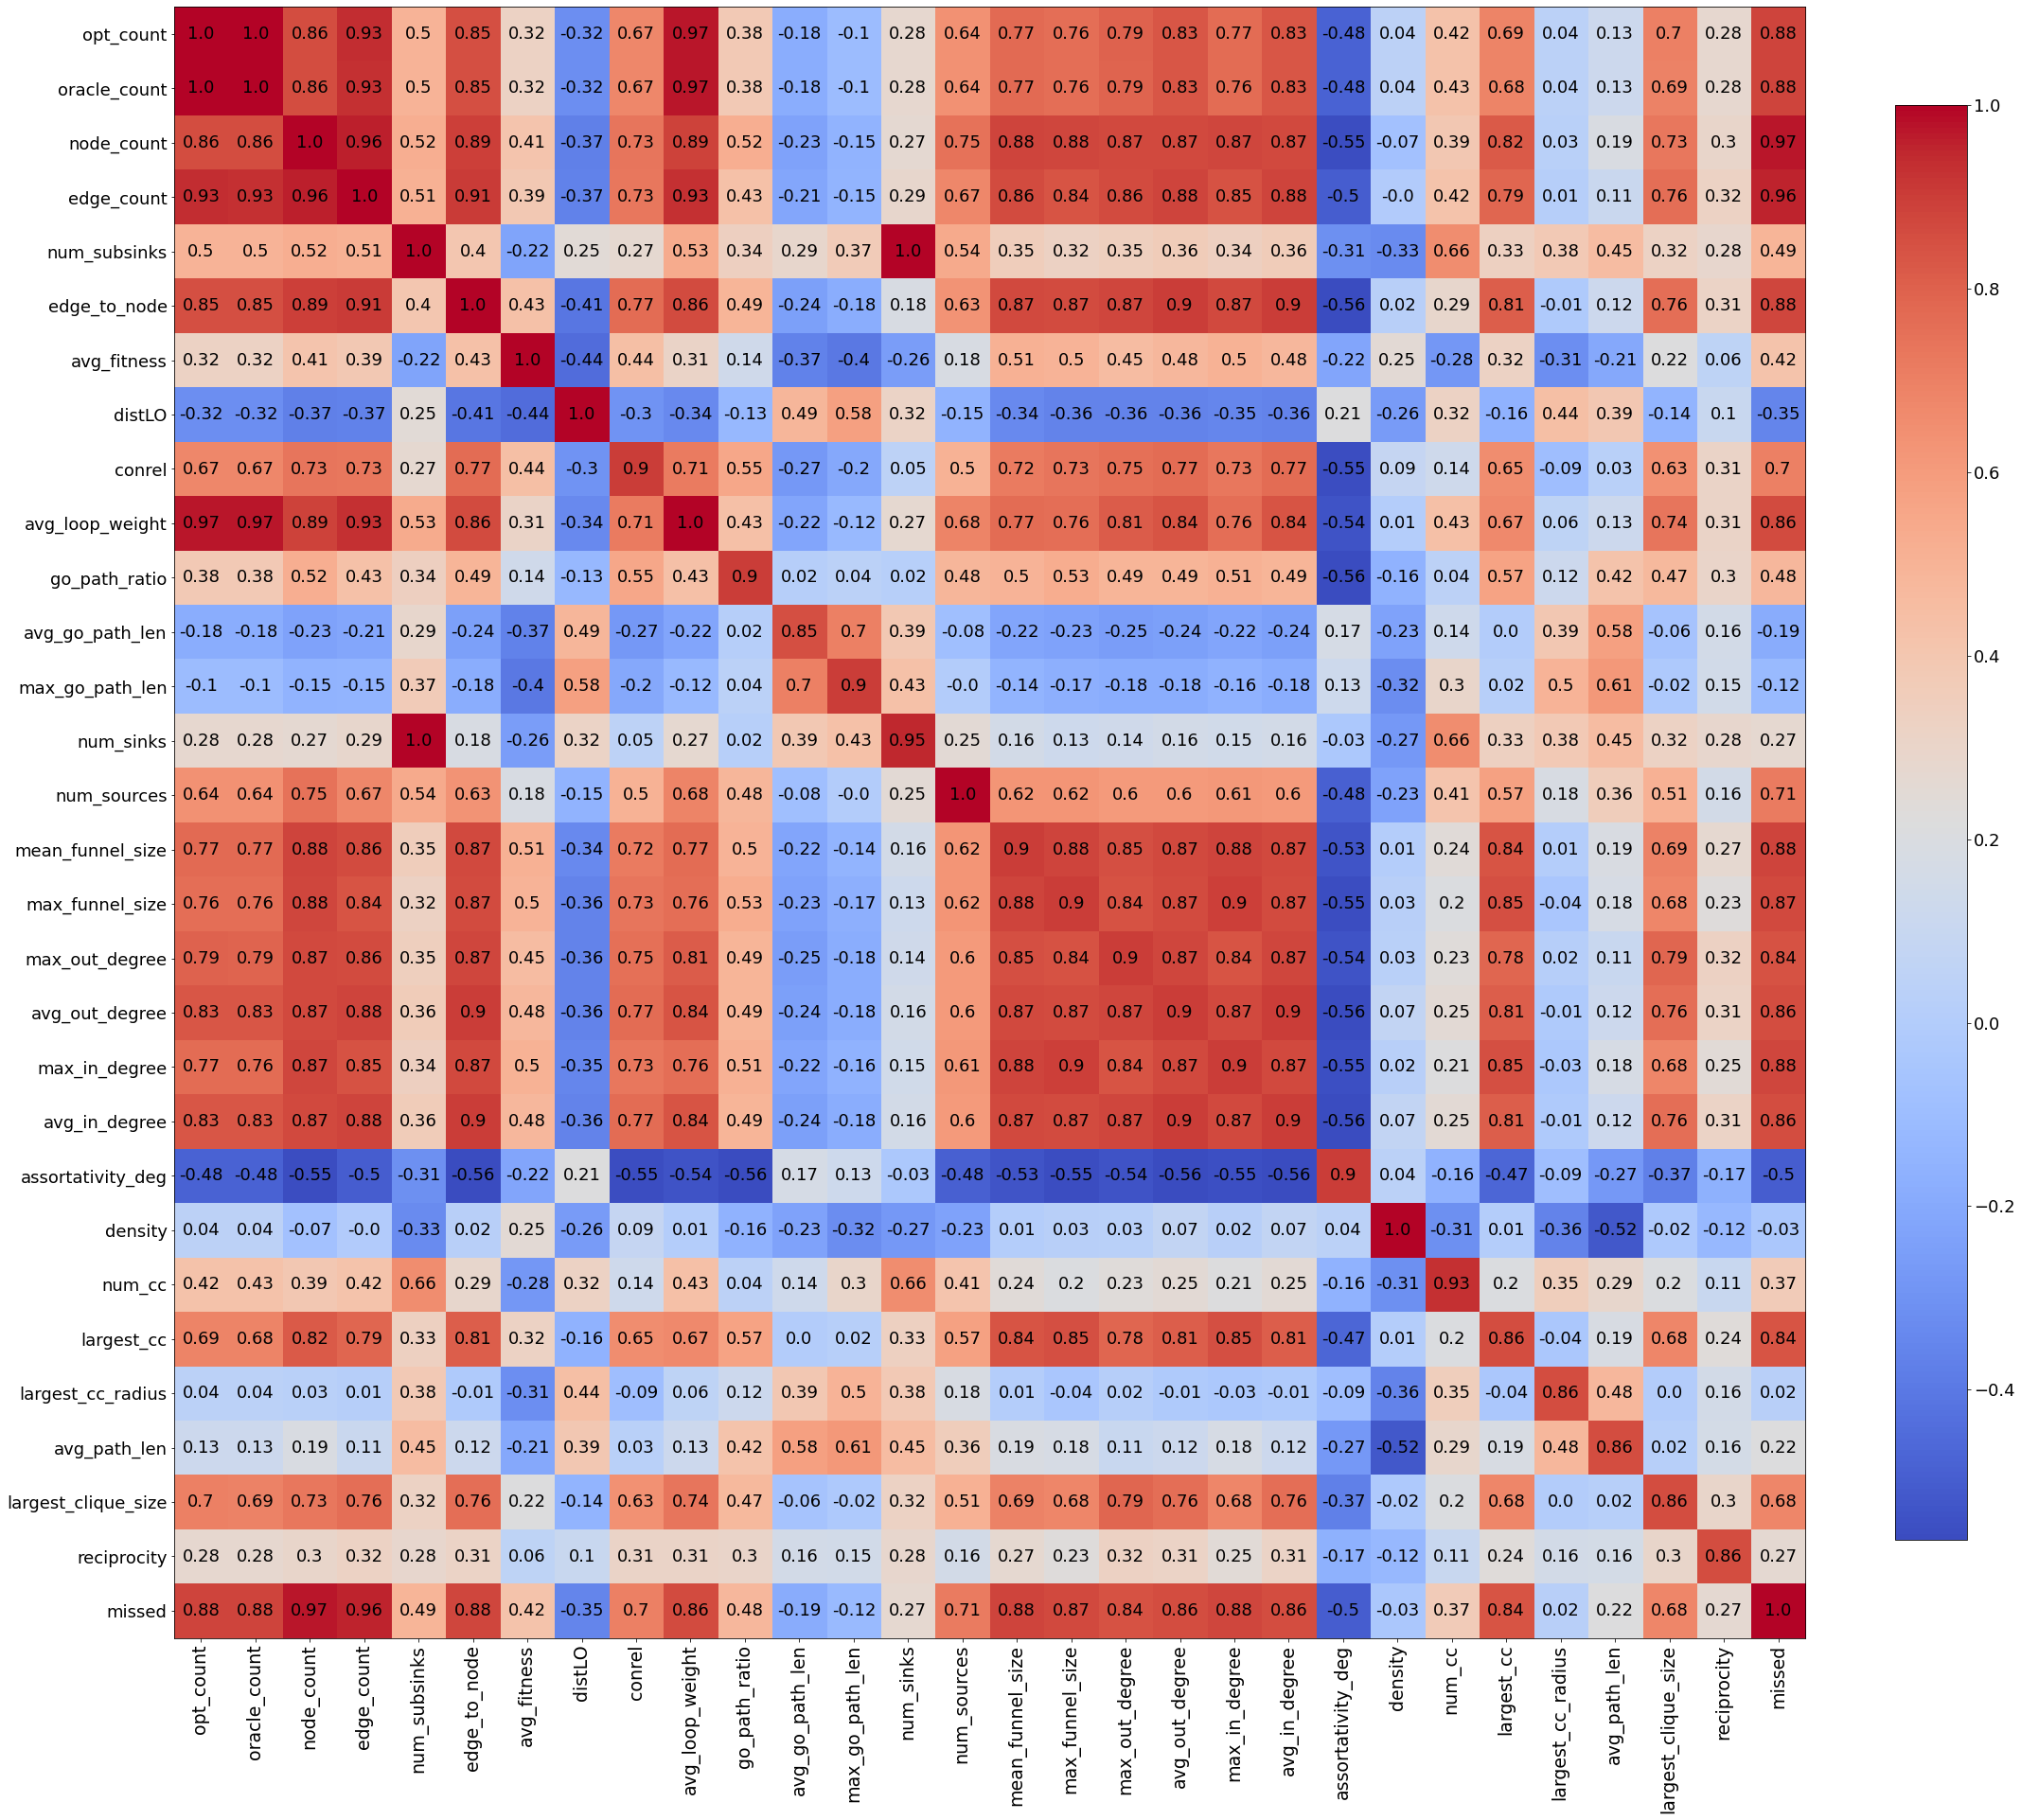
\includegraphics[width=\textwidth]{chapters/experiments/img/twophase_corr.png}
    \caption{Wzajemna korelacja miar - próbkowanie dwufazowe}
    \label{fig:corr_twophase}
\end{figure}
